\documentclass[oneside,onecolumn]{report}

\usepackage[left=2cm,right=2cm,top=2cm,bottom=2cm]{geometry}
\usepackage[colorlinks=false,hidelinks,bookmarksdepth=3]{hyperref}
\usepackage[utf8]{inputenc}
\usepackage{amssymb}
\usepackage{bm}
\usepackage{physics}
\usepackage{mathtools}
\usepackage{graphicx}
\usepackage{cancel}
\usepackage{enumitem}

\newcommand{\ver}[1]{\bm{\widehat{#1}}}
\newcommand{\E}[1]{\text{E} \left\{ #1 \right\}}
\newcommand{\Var}[1]{\text{Var} \left\{ #1 \right\}}
\newcommand{\Cov}[1]{\text{Cov} \left\{ #1 \right\}}
\newcommand{\eps}{\varepsilon}
\newcommand{\inp}[2]{\left\langle #1, #2 \right\rangle}
\DeclareMathOperator*{\argmax}{argmax}
\DeclareMathOperator*{\argmin}{argmin}
\DeclareMathOperator*{\sgn}{sgn}
\DeclareMathOperator*{\pdf}{p}
\let\P\relax
\DeclareMathOperator*{\P}{P}

\title{Recognition systems}
\author{Francesco Zardi}

\begin{document}


\pagenumbering{gobble}
\begin{titlepage}\

        \vfill

        \begin{center}
            \huge \bfseries Notes from the course of \\
        \end{center}

        \begin{center}
            \huge \bfseries Recognition Systems \\
        \end{center}

        \vskip2cm

        \begin{center} \large
            \today
        \end{center}

        \vfill


    \vfill

    {
        \bfseries
        Academic year - 2018/19

        Spring semester
    }
\end{titlepage}


\renewcommand{\thepage}{\roman{page}}
\tableofcontents

\clearpage

\renewcommand{\thepage}{\arabic{page}} % Arabic numerals for page counter
\setcounter{page}{1} % Start page number with 1

% Don't indent paragraphs
\setlength{\parindent}{0cm}


\chapter{Introduction}
\section{Basics of recognition systems}

Data acquisition process
\begin{itemize}
    \item physical process
    \item sensors
    \item sampling
    \item quantization
    \item digital signal
\end{itemize}

False color compositing: non-visible light is mapped onto visible light so that humans can see it

Pattern: vector of features/template/model to generate objects or parts of it

Patterns include random components to various extents, and can thus be completely random or completely deterministic.

Texture pattern: composed of a repeated texels, i.e. smaller elements formed by pixels

The recognition function maps the space of patterns/features/characteristics/parameters to the space of objects with the use of prior knowledge.

Recognition can also be seen as a a partitioning of the feature space into subsets of features that are mapped to the same object.


\subsection{Recognition system block scheme}

\begin{enumerate}
    \item Acquisition: choice of number of sensors, sensitivity, sampling frequency
    \item Pre-processing: calibration of the sensors, noise removal
    \item Feature extraction: choice of the features that have the highest discrimination power, are the least computationally demanding to compute, are the least sensitive to transformation of the input (i.e. rotations, translations, etc)
    \item Classification: choice of the architecture depending on the number of features, amount and typology of noise, prior knowledge
    \item Post-processing: remove easily-spottable classification errors, move the classifier output to a more readable format
    \item Decision
\end{enumerate}


\subsection{Recognition system design steps}

\begin{enumerate}
    \item Collect data
    \begin{itemize}
        \item training samples must be rich
        \item not redundant
        \item representative of the whole feature space
        \item data augmentation through simple transformation of the training samples
    \end{itemize}
    \item Select features
    \item Choose model
    \item Train classifier (i.e. find the parameters of the classifier)
    \item Evaluate classifier
    \begin{itemize}
        \item requires that a portion of the available training samples are not used for training the classifier but exclusively for its evaluation
        \item typical evaluation criteria are accuracy, training time and prediction time
        \item Cross validation: used when we need to evaluate the classifier with few available training samples
        \begin{enumerate}
            \item divide the training samples in N groups
            \item choose one of these groups as the test group
            \item train the classifier on the other groups and then evaluate it using the test group
            \item repeat from 2 choosing a group that hasn’t been chosen as test group yet
        \end{enumerate}
        \item Leave-one-out (LOO): a kind of cross-validation where the groups only comprise 1 test sample
    \end{itemize}
\end{enumerate}


\subsection{Example: Salmon vs sea-bass}

Segmentation: gathering single pixels into regions using some kind of criterion

\begin{enumerate}
    \item  Collect the data: we gather images of salmons and sea-basses

    \item  Features selection:
    \begin{enumerate}
        \item Length of the fish: the two classes overlap, so it is not a very good feature. The pdf of the ideal feature is composed by one Dirac delta for each class. A good real feature has a Gaussian bell for each class, where the variance and the barycenters of the Gaussians are so that the two classes are clearly distinguishable.
        \item Brightness of the fish: better feature
    \end{enumerate}
    \begin{center}
        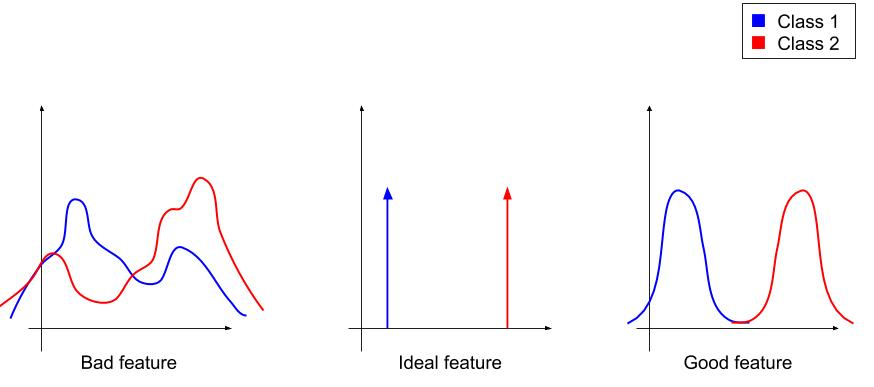
\includegraphics[width=15cm]{bad_feature.jpg}
    \end{center}

    \item Choose model: we choose a simple threshold-based classifier

    \item Train classifier:
    \begin{enumerate}
        \item estimate the threshold T that minimizes the error probability (Minimum error criterion)
        \item sometimes, errors have different importance e.g. they have different costs. In that case, we should use a Minimum cost criterion.
    \end{enumerate}

    \item Evaluate the classifier.
\end{enumerate}


How to improve the system?
\begin{itemize}
    \item We can combine two features together. We will use a 2D linear classifier as model.

    \item We can use a non-linear classifier, but then we might have an over-fitting problem. When a classifier over-fits, it adapts to recognize the training samples and does not work when the samples change slightly. The classifier has actually memorized the training samples instead of their general characteristics. In general, we want to avoid over-fitting because

    \begin{center}
        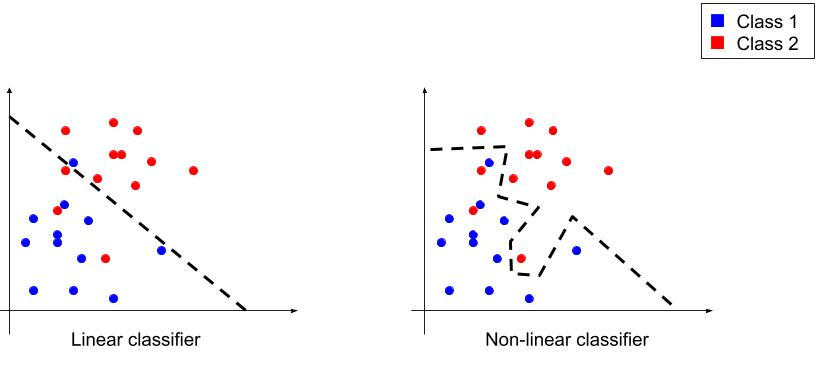
\includegraphics[width=15cm]{2D_linear_classifier.jpg}
    \end{center}

    \begin{itemize}
        \item the ground truth might contain errors (mislabelling)
        \item the classifier can not generalize and correctly address novel patterns
    \end{itemize}

    \item Find new features, maybe with additional sensors. Multi-sensor RSs are not always better, since
    \begin{itemize}
        \item more features might require a higher training and classification time
        \item the new features might not have a significant information content
        \item if the new features are highly correlated with the ones already in use, they might not yield more information
    \end{itemize}
\end{itemize}


\subsection{Regression}
\subsubsection{Known model}

If the statistical model of the data is known, designing a detection system is easy.

Consider a source, which can emit symbols from the alphabet $\{$Yes, No, Maybe$\}$ with equal probability.

To convey this signal over a channel we can use a Pulse Amplitude Modulation (PAM) system, e.g. by sending a signal at 1V, 2V and 3V for Yes, No and Maybe respectively.
Let $x$ be the signal sent over the channel then $p_x(x|\text{Yes})=(x-1\text{V}),p_x(x|\text{No})=(x-2\text{V})$ and $p_x(x|\text{Maybe})=(x-3\text{V})$.

Now imagine that the channel is affected by AWGN with distribution $N(0,2)$. Let $y$ be the signal on the channel, i.e. $y=x+n$.
The distribution of the signal $y$ is given by $p_y(y|\text{Symbol})=p_x(y|\text{Symbol})*p_n(y)$, i.e. $p_y(y|\text{Yes}) \sim N(1\text{V}, 2),p_y(y|\text{No}) \sim N(2\text{V},2)$ and $p_y(y|\text{Maybe}) \sim N(3\text{V},2)$.

Thus if we want to design a detection system, we can simply set 2 thresholds at $T_1=1.5$V and $T_2=2.5$V.
\subsubsection{Unknown model}

However, in practical problems, the model distribution are not known beforehand. However. the data gathered gives a number of samples from the distribution. We can thus try to guess the parameters of the distribution function from the known samples, by applying a process called \textbf{regression}.

The simplest regression is linear regression, where we have a number of points $(x,y)$ and we want to estimate the $a$ and $b$ parameters such that

$$ y = ax + b $$

Consider for examples the points $(1,1), (2,1)$ and $(3,3)$. We can express the problem in matrix form as follows

$$ \bm M \bm \alpha = \bm t $$

where
\begin{itemize}
    \item $\bm M$ is the matrix $3\times2$, with the various $x$ values on the first column and 1 on the second column
    \item $\bm \alpha$ is the column vector containing $a$ and $b$
    \item $\bm T$ is the column vector containing the various $y$ values
\end{itemize}

If the number of  given points is exactly 2, we can find the parameters that yield a line which intersects both points. However if the number of given points is higher, this is not possible (unless all the points are lined). In this case, we want to find the and parameters that yield a line which is \textbf{the closest} to the given points, and does not necessarily pass through them.

More formally, we ought to norm of the error $e$, defined as

$$ \bm e \triangleq \bm M \bm \alpha - \bm t $$

Since $\norm{\bm e}^2$ is convex, the $\bm{\widehat \alpha}$ that minimizes it the one that satisfies

$$ \pdv{e}{\bm{\widehat \alpha}} = 0 $$

Indicating with $\alpha_i$ and $e_i$ the $i$-th element of $\bm \alpha$ and $\bm e$ respectively, then
\begin{align*}
    \pdv{\norm{e}^2}{\alpha_i}
    &= \pdv{}{\alpha_i} \sum_{i = 1}^N e_i^2 \\
    &= \sum_{i = 1}^N \pdv{e_i^2}{\alpha_i} \\
    &= \sum_{i = 1}^N \pdv{e_i^2}{e_i} \pdv{e_i}{\alpha_i} \\
    &= \sum_{i = 1}^N 2 e_i \pdv{\left(M_{i,j} \alpha_i - t_i\right)}{\alpha_i}  \\
    &= 2 \sum_{i = 1}^N e_i M_{i, j}
\end{align*}

Which in matrix form becomes

$$ \pdv{e}{\bm{\widehat \alpha}} = 2 \bm M^T \bm e = 0 $$

Substituting the definition of $\bm e$

\begin{gather*}
    2 \bm M^T \bm e = 0 \\
    \bm M^T (\bm M \bm{\widehat \alpha} - \bm t) = 0 \\
    \bm M^T \bm M \bm{\widehat \alpha} - \bm M^T \bm t = 0 \\
    \bm M^T \bm M \bm{\widehat \alpha} = \bm M^T \bm t \\
    \bm{\widehat \alpha} = \left(\bm M^T \bm M \right)^{-1} \bm M^T \bm t
\end{gather*}

Where the quantity $\left(\bm M^T \bm M \right)^{-1} \bm M^T$ is called \textbf{pseudo-inverse} (sometimes indicated with $\bm M^\#$), and it generalizes the matrix inversion problems for non-square matrices. This system can be generalized to other polynomials (i.e. not just first order), as long as the coefficients have a linear dependency on the data.

\subsubsection{Remote sensing applications}
\begin{itemize}
    \item Gesture recognition
    \item Eye tracking
    \item Cardiac pathology detection trough ECG
    \item Ground penetrating radar
\end{itemize}

Auto-thresholding algorithms: find the threshold that maximizes the compaction

Multi-labelling: more labels are assigned to the same data sample (e.g.: the labels "asphalt" and "pedestrian crossing")

OCR feature: 8 features, 4 vertical strips and 4 horizontal strips

\subsection{Accuracy measures}

\textbf{Accuracy} is defined for every class as

$$ \text{Accuracy(class)} = \frac{\text{\# of samples belonging to class correctly classified}}{\text{overall \# of samples belonging to class}} $$

Given a classifier that supports $N$ classes, its confusion matrix is defined as the $N\times N$ matrix, whose elements at the $i$-th row and $j$-th column is given by the number of samples belonging to the $i$-th class that were classified as to belonging to the $j$-th class.

The \textbf{average accuracy} is defined as
$$ \text{Average accuracy} = \frac{\sum_{i=1}^N \text{Accuracy}(\text{class}_i)}{N} $$

The \textbf{overall accuracy} is instead defined as
$$ \text{Overall accuracy} = \frac{\text{\# of samples correctly identified}}{\text{overall \# of samples}} $$

Note that the overall accuracy is biased by the dominant class, while the average accuracy considers each class as equally important, independently of their occurrence.


\clearpage
\section{Classifiers}

\subsection{Threshold based classifier}
Super simple, quite rigid.
No over-fitting problem when using a linear threshold.

\subsection{k Nearest Neighbour classifier}

The classification algorithm for a kNN classifier is the following

\begin{enumerate}
    \item Given a sample $x$ to classify, compute the distance between $x$ and all the training samples
    \item Choose the $k$ training samples which are closest to $x$
    \item Classify $x$ as belonging to the class that is dominating the $k$ samples extracted (i.e. the most common class among them)
\end{enumerate}

A kNN classifier requires no training, as it actually just remembers all the training samples.

In order to define a kNN classifier we need to choose
\begin{itemize}
    \item the $k$ hyper-parameter
    \item the distance function
\end{itemize}

A kNN can be quite computationally inefficient as $k$ grows.


\clearpage
\chapter{Statistical estimation theory}
\section{Introduction to statistical estimation}

We can categorize signals as follows:

\begin{enumerate}
    \item noisy deterministic signals: the signal is completely known, but affected by noise
    \item noisy parametric signals: the signal is partially known (e.g.: except for a number of parameters) and affected by noise
    \item noisy random signal: the estimation can only rely on the available observations
\end{enumerate}


The goal of statistical estimation is that of deriving a statistical model for a stochastic process from a set of observation.

More formally, suppose we have $n$ features $\bm x$ with unknown pdf.
Let $\bm X$ be a finite set of $\bm N$ i.i.d. observations or samples, called training samples.
The objective is to find as estimated pdf $\widetilde \pdf(\bm x)$ based on the available samples $\bm x$ which is as close as possible to the actual pdf $\pdf(\bm x)$.

We can categorize statistical estimation methods in two main categories.
\begin{itemize}
    \item Parametric: the model/shape of the pdf is known but not it's parameters.
    \begin{itemize}
        \item Maximum likelihood
        \item Bayesian estimation
    \end{itemize}
    \item Non-parametric:
    \begin{itemize}
        \item kNN
        \item Parzen window
        \item Orthogonal function approximation
    \end{itemize}
\end{itemize}


\section{Estimator evaluations}

\subsection{Biased and consistent estimators}
The estimate is random variable that depends on the observation matrix $\bm X$.
We define the estimation error $\bm \eps$ as
$$ \bm \eps \triangleq \bm{\widehat \theta} - \bm \theta $$

The \textbf{ideal} estimator should, for each element $\eps_i$ of $\bm \eps$,
\begin{itemize}
    \item be unbiased, i.e. $\lim_{N \to +\infty} \E{\bm \eps} = \bm 0$
    \item be consistent, i.e. $\lim_{N \to +\infty} \P(\norm{\eps} < \delta) = 1 \quad \forall \delta > 0$
\end{itemize}
The necessary condition for consistency is that
$$ \lim_{N \to +\infty} \E{\bm \eps} = \bm 0 \quad \wedge \quad \lim_{N \to +\infty} \Var{\bm \eps} = \bm 0 $$

\subsubsection{Variance of an unbiased estimator}
In order to asses the variance, the Cramér-Rao bound is used, which expresses a lower bound for the variance of an unbiased statistical estimated as

$$ \Var{\eps_i} \geq [I(\bm\theta)]_{i, i}^{-1} $$

i.e. $\Var{\eps_i}$ is greater or equal to the $i$-th value of the diagonal of $I(\theta)$, which is the Fisher information matrix, given by

$$ I(\bm \theta)_{i, j} = \E{
\pdv{\ln(\pdf(\bm X | \bm \theta))}{\theta_i}
\pdv{\ln(\pdf(\bm X | \bm \theta))}{\theta_j}
} $$

When the Cramér-Rao bound is reached, the estimator is said to be \textbf{efficient}.

\subsubsection{Asymptotic properties}
We can evaluate the intrinsic goodness of an estimator by evaluating its behaviour when the number of available samples is unlimited.
This is referred to as \textbf{asymptotic behaviour}.

An estimator is asymptotically unbiased if
$$ \lim_{N \to +\infty} \E{\bm \eps} = \bm 0 $$

An estimator is asymptotically efficient  if
$$ \lim_{n \to +\infty} \Var{\bm \eps} = [I(\bm\theta)]_{i, i}^{-1} $$

An estimator is consistent if
$$ \lim_{n \to +\infty} \P(\norm{\bm \varepsilon} < \delta) = 1 \quad \forall \delta $$




\section{Maximum likelihood estimation}
Assume that the model of $\pdf(\bm x)$ is characterized by $r$ parameters $\bm \theta = (\theta_1, \ldots, \theta_r)$.
The dependency of the model on $\bm \theta$ is highlighted by the following notation

$$ \pdf(\bm X | \bm \theta) $$

We define the \textbf{likelihood function} as the probability of observing the samples $\bm X = \{X_1, \dots X_M\}$ when the stochastic process generating the samples follows the pdf with parameters $\bm \theta$.

$$ \pdf(\bm X | \bm \theta) = \prod_{k = 1}^M \pdf(X_k | \bm \theta) $$

The correct parameters $\bm{\widehat \theta}$ can then be estimated as those maximizing the likelihood function.

The ML estimation is
\begin{itemize}
    \item asymptotically unbiased
    \item asymptotically efficient
    \item consistent
\end{itemize}


Example:

In the case of a gaussian distributed pdf, $\bm \theta = (\mu, \sigma)$.

The likelihood function is then
\begin{align*}
    \pdf(\bm X| \bm \theta)
    &= \prod_{k = 1}^M \pdf(X_k | \bm \theta) \\
    &= \prod_{k = 1}^M \frac{1}{\sqrt{2 \pi} \sigma} \exp( -\frac{(X_k - \mu)^2}{2 \sigma^2}) \\
    &= \left(\frac{1}{\sqrt{2 \pi} \sigma}\right)^N \exp( - \sum_{n -1}^N \frac{(X_k - \mu)^2}{2 \sigma^2}) \\
    &=  \frac{1}{\sqrt{2 \pi} \sigma_\text{tot}} \exp( - \sum_{n -1}^N \frac{(X_k - \mu_\text{tot})^2}{2 \sigma_\text {tot}^2} )
\end{align*}

Thus we got another gaussian! Now $\bm{\widehat \theta}$ can be found as the value maximizing this function.

\subsection{Model selection}

There are many models that can be chosen for Maximal Likelihood estimation
\begin{itemize}
    \item Gaussian: the most used, because the sum of i.i.d. variables has gaussian distribution (when its variance is finite), due to the central limit theorem
    \item Generalized gaussian
    \item Gamma: often used to model speckle noise
    \item Rayleigh
    \item Chi-square
\end{itemize}

Common parameters for these models are:
\begin{itemize}
    \item Mean
    \item Variance
    \item Skewness: asymmetry around the mean
    \item Kurtosis: how square is the shape rather than triangular/spiky
\end{itemize}


\subsubsection{Multivariate pdf}

The pdf models mentioned before can be multi-dimensional.
We will consider now the case of an $N$-dimensional gaussian distribution.

In this case, the distribution of an $N$ dimensional value $\bm x$ is defined by an $N \times 1$ mean vector $\bm m$, and the $N \times N$ covariance matrix $\bm \Sigma$, defined as

$$ \bm \Sigma = \Cov{\bm x} = \E{(\bm x - \bm \mu_x)(\bm x - \bm \mu_x)^T} = \E{\bm x \bm x^T} - \bm m \bm m^T $$

The covariance matrix
\begin{itemize}
    \item is symmetrical
    \item is positive semi-definite (i.e. has only non-negative eigenvalues)
    \item presents the variance $\sigma_i^2$ of the $i$-th variable of $\bm x$ at the $i$-th position of its diagonal
    \item is diagonal if the variables $\bm x$ are iid
\end{itemize}

When plotted, the pdf of a 2D dimensional gaussian resembles a bell.
We can define isolevels as the points of the bell that correspond to $\bm x$ values with the same probability.

The isolevels identify ellipses on the bell.
The eigenvectors of the covariance matrix identify the axes of these ellipses.
In particular, the eigenvector corresponding to the highest eigenvalue identifies the main axis.

There are some special cases:
\begin{itemize}
    \item when the variables $\bm x$ are iid. and with the same variance, the covariance matrix is diagonal and its 2 eigenvalues are the same. Thus the isolevels identify circles instead of ellipses.
    \item when the variables $\bm x$ are iid. and with different variance, the covariance is diagonal but with 2 different eigenvalues. The axes of the ellipses are parallel to the $x$ and $y$ axis.
    \item If the gaussian bell is flat, i.e. a single slice, it means that $x_1 = x_2$
    \item If the gaussian bell is flat, but the slice cuts the 2nd and 4th quadrants, it means that $x_1 = -x_2$
    \item If the axes of the gaussian bell are not parallel to the $x$ and $y$ plane, it means that the features are correlated, but not the same.
\end{itemize}

For 3D gaussian distributions, the isolevels are hyper-ellipses, i.e. surfaces shaped like rugby balls. The centre of the hyper-ellipses is the point where the probability density is highest.

\subsubsection{ML estimation behaviour with limited samples}
The estimated mean $\widehat{\bm m}$ and covariance $\bm{\widehat \Sigma}$ of an $n$-dimensional gaussian distribution, computed with the Maximum Likelihood strategy are
$$ \widehat{\bm m} = \frac{1}{N} \sum_{k = 1}^N \bm x_k = \overline{\bm x}
\qquad
\bm{\widehat \Sigma} = \frac{1}{N} \sum_{k = 1}^N \bm x_k \bm x_k^T - \widehat{\bm m} \widehat{\bm m}^T $$

where $\bm X = \{\bm x_1, \bm x_2, \dots, \bm x_N\}$ is the set of the $N$ available training samples.

It can be shown that,
\begin{itemize}
    \item The ML estimation is not biased when estimating $\widehat{\bm m}$
    $$ \E{\widehat{\bm m}} = \bm m $$

    \item The ML estimation is biased when estimating $\widehat{\bm \Sigma}$
    $$ \E{\widehat{\bm \Sigma}} = \frac{N - 1}{N} \bm \Sigma $$
\end{itemize}

In order to have an unbiased estimation of $\widehat{\bm \Sigma}$ even with a limited number of samples $N$, we can change the formula for the estimation of $\widehat{\bm \Sigma}$ as follows
$$ \widehat{\bm \Sigma}_\text{unbiased} = \frac{N}{N - 1} \widehat{\bm \Sigma} $$

Thus
$$ \E{\widehat{\bm \Sigma}_\text{unbiased}}
= \frac{N}{N - 1} \E{\widehat{\bm \Sigma}}
= \frac{N}{N - 1} \frac{N - 1}{N} \bm \Sigma
= \bm \Sigma $$


\section{Bayesian estimation}
The main difference between Bayesian and Maximum Likelihood estimation is that the former treats the model's parameters themselves as stochastic variables.

Moreover, through Bayesian estimation we don't compute an estimate of the parameters of the model, but we compute the distribution itself.
The distribution is computed by averaging all the different pdf values obtained with the specified model, but using different parameters.
The average is weighted by the posterior probability associated the specific value of the parameters used.

Assume that
\begin{itemize}
    \item the initial knowledge/prior on $\bm \theta$ is contained in the density $\pdf(\bm \theta)$ (e.g. if we know that $\theta_1$ should be within an interval $[a, b]$, then we set $\pdf(\theta_1)$ to a uniform distribution within that interval).
    \item The model of pdf to be estimated $\pdf(x|\bm \theta)$ except a certain number of parameters
    \item A number $N$ of training samples is given
\end{itemize}

We want to compute the pdf estimate $\widehat \pdf(x)$.
We can express its relation from the set $X$ of the given training sample with the following notation
$$ \widehat \pdf(x) = \pdf(x | X) $$

Let us introduce $\bm \theta$ so that
$$ \widehat \pdf(x) = \pdf(x | X) = \int \pdf(x, \theta | X) \dd \theta $$

By applying Bayes' theorem
$$ \widehat \pdf(x)
= \int \pdf(x, \theta | X) \dd \theta
= \int \pdf(x | \theta, X) \pdf(\theta | X) \dd \theta
$$

However, if $\theta$ is given, then the distribution of $x$ does not depend on $X$.
Thus $\pdf(x, \theta | X) = \pdf(x, \theta)$, and
$$ \widehat \pdf(x) = \int \underbrace{\pdf(x | \theta)}_{\substack{\text{parametric} \\ \text{model}}} \underbrace{\pdf(\theta | X)}_{\substack{\text{posterior} \\ \text{probability}}} \dd \theta $$

Here, the parametric model represents the information regarding the distribution to be estimated.
Instead, the posterior probability is given by
$$ \pdf(\bm \theta | X) = \frac{\overbrace{\pdf(X | \bm \theta)}^\text{likelihood} \overbrace{\P(\bm \theta)}^\text{prior}}{\underbrace{\pdf(X)}_\text{marginal likelihood}} $$

and thus represents
\begin{itemize}
    \item the likelihood function, i.e. the information conveyed by the training samples,
    \item the prior, i.e. the prior knowledge on the parameters,
    \item the marginal likelihood.
\end{itemize}

So, for example, when computing $\widehat \pdf(x)$ for a gaussian parametric model, we average all the possible gaussian models, but weighing every contribution on the basis of the posterior probability.


\section{kNN and PW estimators}
\subsection{Introduction}

Non-parametric estimators are chosen when
\begin{itemize}
    \item the stochastic process to estimate does not fit any model
    \item we have no prior knowledge of the stochastic process to estimate
\end{itemize}

Let $x^*$ be a generic sample, and $R$ a predefined region of the sample space such that $x^* \in R$.
Assume that $R$ is small enough so that $\pdf(x)$ is constant $\forall x \in R$.

Moreover, the probability that a sample $x$ falls into the $R$ region should be
$$ \pdf(x \in R) = \int_R \pdf(x) \dd x = \pdf(x) V $$
where $V$ is the volume of $R$.
We can rewrite this as a relative frequency
$$ \pdf(x \in R) = \frac{k}{N} $$
where $k$ is the number of samples in $R$, and $N$ the overall number of samples.

For $N \to +\infty$,
$$ \lim_{N \to +\infty} \left( \abs{\widehat p_r - p_r} < \delta \right) = 1 \quad \forall \delta > 0 $$
thus the estimation is consistent.

We can also take into account the ``volume'' $V$ of $R$, so
$$ \pdf(x \in R) = \frac{k}{N V} $$

This leads to to two non-parametric estimator systems
\begin{enumerate}
    \item kNN estimator: fix $k$, $V$ is computed using the training samples
    \item Parzen window: fix $V$, $k$ is computed using the training samples
\end{enumerate}

\subsection{Example: Univariate Gaussian model estimation}
Assume we want to estimate the pdf of a univariate gaussian distribution with known variance $\sigma^2$.

First, we compute the posterior probability
$$ \pdf(\mu | X) = \frac{\pdf(X | \mu) \pdf(\mu)}{\pdf(X)} $$

Disregarding $\pdf(X)$, and assuming that $\mu$ follows a Gaussian distribution with parameters $\mu_0, \sigma_0^2$
\begin{align*}
\pdf(\mu | X)
& \propto \pdf(X | \mu) \pdf(\mu) \\
&= \left[ \prod_{k = 1}^N \frac{1}{\sqrt{2 \pi \sigma^2}} \exp( - \frac{(x_k - \mu)^2}{2 \sigma^2}) \right]
\left[ \frac{1}{\sqrt{2 \pi \sigma_0^2}} \exp( - \frac{(\mu - \mu_0)^2}{2 \sigma_0^2}) \right] \\
&\propto \exp( - \frac{(x_k - \mu)^2}{2 \sigma^2} - \frac{(\mu - \mu_0)^2}{2 \sigma_0^2}) \\
&= \exp( - \sum_{k = 1}^N \frac{(x_k - \mu)^2}{2 \sigma^2} - \frac{(\mu - \mu_0)^2}{2 \sigma_0^2}) \\
&= \exp( - \sum_{k = 1}^N \frac{x_k^2 - 2 x_k \mu + \mu^2}{2 \sigma^2} - \frac{\mu^2 - 2 \mu_0 \mu + \mu_0^2}{2 \sigma_0^2}) \\
&= \exp( - \sum_{k = 1}^N \frac{x_k^2 - 2 x_k \mu + \mu^2}{2 \sigma^2} - \frac{\mu^2 - 2 \mu_0 \mu + \mu_0^2}{2 \sigma_0^2}) \\
&= \exp( - \sum_{k = 1}^N \frac{x_k^2}{2 \sigma^2} - \frac{\mu_0^2}{2 \sigma_0^2})
\exp(
- \frac{1}{2} \mu^2 \left[ \sum_{k = 1}^N \frac{1}{\sigma^2} + \frac{1}{\sigma_0} \right]
+ \mu \left[ \sum_{k = 1}^N \frac{x_k}{\sigma^2} + \frac{\mu_0}{\sigma_0^2} \right])
\end{align*}

The product of two gaussian functions is yet another gaussian, so we expect that
\begin{align*}
\pdf(\mu | X)
&\propto \frac{1}{\sqrt{2 \pi \sigma_N^2}} \exp( - \frac{(x_k - \mu_N)^2}{2 \sigma_N^2}) \\
&= \frac{1}{\sqrt{2 \pi \sigma_N^2}} \exp( - \frac{(x_k - \mu_N)^2}{2 \sigma_N^2})
\end{align*}

(MISSING)




\subsection{kNN estimator}
In order to compute an estimate $\widehat \pdf(x^*)$ of the probability $\pdf(x^*)$ of a given sample $x^*$, follow these steps:
\begin{enumerate}
    \item Find the $k$ test samples that are closest to $x^*$
    \item Compute the volume $V$ of the region $R$ that has a predefined shape and is centered at $x^*$
    \item Compute $\widehat \pdf(x^*)$ as
    $$ \widehat \pdf(x^*) = \frac{k}{N V} $$
\end{enumerate}

The hyper-parameters of the kNN estimator are
\begin{itemize}
    \item $k$
    \item the shape of the region $R$
\end{itemize}

It can be shown that if $k$ is chosen as a function of $N$, a necessary and sufficient condition for the kNN estimator to be consistent is the following
$$ \lim_{N \to +\infty} k(N) = +\infty \quad \wedge \quad \lim_{N \to +\infty} \frac{k(N)}{N} = 0 $$
i.e. the region should comprise a large number of samples as the number of available samples grows to infinity and also the region should comprise a small number of samples compared to the number of available samples, as the latter grows to infinity.

A function $k(N)$ that satisfies both these constraints is
$$ k(N) = \sqrt{N} $$


\subsection{Parzen window estimator}
In order to compute an estimate $\widehat \pdf(x^*)$ of the probability $\pdf(x^*)$ of a given sample $x^*$, follow these steps:
\begin{enumerate}
    \item Define the region $R$ of volume $V$ having a predetermined shape and centered in $x^*$
    \item Count the number $k$ of test samples that fall into the region $R$
    \item Compute $\widehat \pdf(x^*)$ as
    $$ \widehat \pdf(x^*) = \frac{k}{N V} $$
\end{enumerate}

Let's assume that we choose a $n$-dimensional hyper-cube of edge $h$ as the shape of the region $R$.
Its volume $V$ will then be given by
$$ V = h^n $$

The analytical expression for computing $k$ can be described by using a window function
$$ \gamma(x) = \begin{cases}
    1 & \text{if } x \in R \\
    0 & \text{otherwise}
\end{cases} $$

Then, the training sample $x_k$ belongs to the region $R$ centered in $x^*$ if
$$ \gamma \left( \frac{x_k - x^*}{h} \right) = 1 $$

Thus, $\widehat \pdf(x^*)$ is given by
$$ \widehat \pdf(x^*)
= \frac{k}{N V}
= \frac{1}{N h^n} \sum_{k = 1}^N \gamma \left( \frac{x_k - x^*}{h} \right) $$
where $N$ is the number of available training samples.


\subsubsection{Window function selection}
We can also give another interpretation of the formula.
Instead of considering a single window function centered at $x^*$, consider $N$ replicas of the window function centered at $x_k, k = 1, \dots, N$.

The value of $\widehat \pdf(x^*)$ is then given by summation of all the window functions in $x^*$.

Thanks to this interpretation, it is clear that the smoothness of the estimated pdf depends on the shape of the window function.

The window function can be chosen arbitrarily, subject to the two following constraints:
\begin{itemize}
    \item $\widehat \pdf(x^*)$ should be non-negative,
    \item $\widehat \pdf(x^*)$ should integrate to 1.
\end{itemize}
A window function satisfies these conditions if it is itself a valid density function, i.e.
$$ \begin{dcases}
    \gamma(x) \geq 0 \quad  \forall x \in \mathbb R \\
    \int_R \gamma(x) \dd x = 1
\end{dcases} $$

Other appreciable properties of a good window functions are the following
\begin{itemize}
    \item $\gamma(x)$ should have its global maximum at $x = 0$
    \item $\gamma(x)$ should be continuous
    \item $\displaystyle \lim_{x \to +\infty} \gamma(x) = 0$
\end{itemize}

Window functions are also referred to as \emph{kernels}.
Typical choice of kernels are:
\begin{itemize}
    \item gaussian function
    \item rectangle function
    \item triangle function
    \item exponential function (spiky gaussian)
    \item Cauchy function
    \item sinc squared function
\end{itemize}

\subsubsection{h selection}
Depending on the value of $h$, we can over-smooth or under-smooth the estimated pdf.

\subsubsection{Estimator bias}
What is the bias of a kNN estimator for a given sample $x$?
$$ \E{\widehat \pdf(x)}
= \E{\frac{1}{N V} \sum_{k = 1}^N \gamma \left( \frac{x_k - x}{h} \right)}
= \frac{1}{N V} \sum_{k = 1}^N \E{\gamma \left( \frac{x_k - x}{h} \right)}
$$

Here, the $x$ parameter is fixed, while $x_k$ are $N$ stochastic variables.
Assuming that $x_k, k = 1, \dots, N$ are i.i.d. and distributed as $y$, then
\begin{align*}
    \E{\widehat \pdf(x)}
    &= \frac{1}{N V} N \E{\gamma \left( \frac{y - x}{h} \right)} \\
    &= \frac{1}{V} \E{\gamma \left( \frac{y - x}{h} \right)} \\
    &= \frac{1}{V} \int_{-\infty}^{+\infty} \gamma \left( \frac{y - x}{h} \right) \pdf(y) \dd y
\end{align*}

Note that the integral represents the convolution operation.
$$ \E{\widehat \pdf(x)} = \frac{1}{V} \pdf(y) * \gamma \left( \frac{x}{h} \right) $$

Note that, for $h \to 0$, then $\gamma(x) \to \delta(x)$, thus
$$ \lim_{h \to 0} \E{\widehat \pdf(x)} = \frac{1}{V} \pdf(y) * \delta(x) = \frac{1}{V} \pdf(y) $$

Thus the kNN estimator is biased and asymptotically unbiased.

\subsubsection{Estimator variance}
It can be shown that
$$ \Var{\widehat \pdf(x)}
= \E{\left( \widehat \pdf(x) - \E{\widehat \pdf(x)} \right)^2}
= \frac{\sup \left\{ \gamma(\cdot) \right\} \E{\widehat \pdf(x)}}{N h^n} $$

Thus, to decrease the variance, we want to make $h^n = V$ as big as possible.
It makes sense intuitively, since with larger $h$, the estimate is always the same, and thus its variance is low (even though it may be biased!).

We can demonstrate that it is sufficient that $N V$ is big instead of just $V$.
In particular,
\begin{itemize}
    \item for the estimator to be asymptotically unbiased
    $$ \lim_{N \to +\infty} h(N) = 0 $$
    \item for the estimator to be asymptotically consistent
    $$ \lim_{N \to +\infty} N h(N)^n = 0 $$
\end{itemize}

A function $h(N)$ that satisfies both the above conditions is
$$ h(N) = \frac{1}{\sqrt[2n]{N}} $$

A commonly used kernel in the Parzen window estimation is the Guassian kernel with spherical symmetry.
However, in order to use the symmetrical window, the features along every dimension needs to be normalized.


\section{Orthogonal Function Approximation}
Estimate the unknown, true pdf $\pdf(x)$ in a different space, obtained with a set of basis function.
The problem is finding the basis function and the coefficients of $\pdf(x)$ in that basis.

Let us define the scalar product between two functions $f(x), g(x)$ as
$$ \langle f, g \rangle = \int u(x) f(x) g(x) \dd x $$
where $u(x)$ is the so-called weighting function.

Moreover, we define the norm of a function $f$ as
$$ \norm{f}^2 = \langle f, f \rangle $$

Given the basis functions $\psi_1, \dots, \psi_m$, then the estimated pdf is
$$ \widehat \pdf(x) = \sum_{i = 1}^m c_i \psi_i(x) $$

How do we find the coefficients $c_1, \dots, c_m$ that minimize the norm $d$ of the estimation error $\widehat \pdf(x) - \pdf(x)$?
Let us write $d$ as a function of the coefficients
\begin{align*}
    d
    &= \norm{\widehat \pdf(x) - \pdf(x)}^2 \\
    &= \norm{\sum_{i = 1}^m c_i \psi_i(x) - \pdf(x)}^ 2 \\
    &= \left\langle \sum_{i = 1}^m c_i \psi_i(x) - \pdf(x), \sum_{i = 1}^m c_i \psi_i(x) - \pdf(x) \right\rangle \\
    &= \left\langle \sum_{i = 1}^m c_i \psi_i(x), \sum_{i = 1}^m c_i \psi_i(x) \right\rangle
    + 2 \left\langle \sum_{i = 1}^m c_i \psi_i(x), \pdf(x) \right\rangle
    + \langle \pdf(x), \pdf(x) \rangle
\end{align*}

Assume that the basis functions are orthogonal, i.e.
$$ \langle \phi_i(x), \phi_j(x) \rangle = \begin{cases}
    A_i & \text{if } i = j \\
    0   & \text{otherwise}
\end{cases} $$

Then the expression above becomes
$$ d = \sum_{i = 1}^m c_i^2 A_i - 2 \sum_{i = 1}^m c_i \langle \phi_i(x), \pdf(x) \rangle + \norm{\pdf(x)}^2 $$

Since we want to choose the coefficients $c_1, \dots, c_m$ that minimize $d$, we'll take the partial derivative of $d$ wrt $c_i$, and set it to 0.
$$ \pdv{d}{c_j} = 2 c_j A_j - 2 \langle \phi_j(x), \pdf(x) \rangle = 0 $$

Thus, solving for $c_j$
$$ c_j = \frac{\langle \phi_j(x), \pdf(x) \rangle}{A_j} \quad \text{for } j = 1, \dots, m $$

However, computing the optimal $c_j$ requires knowledge of $\pdf(x)$, which we're trying to estimate!
Let's expand the expression for the optimal $c_j$
$$ c_j
= \frac{1}{A_j} \int u(x) \phi_j(x) \pdf(x) \dd x
= \frac{1}{A_j} \E{u(x) \phi_j(x)} $$

We can approximate the expected value by using the known training samples $x_1, \dots, x_N$, which are
$$ c_j
\approx \frac{1}{A_j} \frac{1}{N} \sum_{k = 1}^N u(x_k) \phi_j(x_k) $$

\subsection{Deriving a set of 2D basis functions}
Suppose we need a set of basis functions $\Psi_{1, 1}(x_1, x_2), \dots, \Psi_{n, n}(x_1, x_2)$ to describe a 2D space.
We can do so by using a set of 1D basis functions $\psi_1(x), \dots, \psi_n(x)$ as shown next

$$ \Psi_{i, j}(x_1, x_2) = \psi_i(x_1) \psi_j(x_2) \quad \text{for } i, j = 1, \dots, n $$

\subsubsection{Choice of basis functions}
Two common basis functions are
\begin{itemize}
    \item Hermite polynomials: they are defined over the whole $\mathbb R$.
    They require the use of a weighting functions to be orthogonal.

    \item Laguerre polynomials: they are defined in the $[0, +\infty)$ interval of $\mathbb R$.
    They also require the use of a weighting function to be orthogonal.
\end{itemize}


\section{Expectation maximization}
More like a framework rather then a method.
It is used for
\begin{itemize}
    \item addressing the incomplete data problem: some of the data available is not 2D as expected but only has 1D (e.g. one of the 2 sensors used was shut down). Thus the second variable is itself an unknown.
    \item estimating a multi-modal distribution: we know that a distribution has a number of modes, and each mode depends on a variable which is not known. This can be considered a form of incomplete data problem.
\end{itemize}

We would like to maximize the likelihood function.
But in the incomplete problem, the likelihood function is itself a random process, since it depends on variables that are not known.
However, we can try to maximize its average.

Assume that the function to maximize is a sum of $M$ gaussian modes, each with parameters $\mu_i, \sigma_i^2$ and weighted by a coefficient $A_i$.

The algorithm for EM is the following:
\begin{enumerate}
    \item Find the $A_j$ coefficients;
    \item Based on the result of the previous step, find the $\mu_i, \sigma_i^2$ values;
    \item Go back to step 1 until the solution converges.
\end{enumerate}


\clearpage
\chapter{Features}
\section{Feature reduction}
It is not unusual to ideal with hundreds of features.
But, after a certain point, adding new features doesn't yield higher accuracy.
This is referred to as Hughes effect.

We can have a hint of why this happens by studying how the ratio between the volume of an $n$-dimensional hyper-sphere and the volume of an $n$-dimensional hyper-cube circumscribed to the hyper-sphere.
As $n$ increases, the ratio decreases substantially, has the mass/volume of the hyper-cube is concentrated close to the corners.

Hughes studied the bias classifier (which are ideal in that they are based on the actual pdf).

Feature reduction aims at
\begin{itemize}
    \item minimizing the number of features,
    \item while keeping the discrimination capabilities higher
\end{itemize}

The result of feature reduction is
\begin{itemize}
    \item an increase in accuracy, and
    \item a reduction of the computational requirements.
\end{itemize}

There are two main approaches at feature reduction
\begin{itemize}
    \item feature reduction by selection (aka feature selection)
    \item feature reduction by transformation (aka feature extraction)
\end{itemize}

\subsection{Problem formulation}
Let $F = \{ x_1, \dots, x_2 \}$ be the set of $n$ available features.
Denote with $f_k$ and $f_{\overline k}$ the $k$-th selected and discarded features.

The goal is to select a subset $F^*$ of $F$ comprising $m < n$ features such that
$$ F^* =\underset{\substack{ F' \subseteq F, \\  \text{card}\{F'\} = m}}{\text{arg max}} \left\{ J(F') \right\} $$
where $\text{card}\{F'\}$ is the cardinality of $F'$.

where $J(\cdot)$ is a function that measures the separability between the classes in the space defined by the considered subset of features.

Feature selection methods:
\begin{itemize}
    \item Wrapping: measure the accuracy of a specific classifier when a particular feature is used. (As it is optimized on one classifier, it is not guaranteed to work in general)
    \item Filtering: use a measure which is not related to the classifier. (More general applicability, but not related to the classifier)
    \item Embedded: the feature selection is part of the training
\end{itemize}

\subsection{Separability measures}

\subsubsection{Divergence measure}
Assume that we know the class-conditional densities $\pdf(x | \omega_i), i = 1, \dots, N$, for all the $N$ classes considered.

The idea is to measure the separability as the overlap between the two distributions.
We could use the ratio between the two class-conditional distributions, but it is not symmetric.
Moreover, we don't want to compute a value point-by-point, but rather have an average.

The divergence measure between the $i$-th and $j$-th class is defined as
\begin{align*}
D_{i j}
&\triangleq \E{\ln( \left. \frac{\pdf(x | \omega_i)}{\pdf(x | \omega_j)} \right| \omega_i)} +
\E{\ln( \left. \frac{\pdf(x | \omega_i)}{\pdf(x | \omega_j)} \right| \omega_j)} \\
&= \int_{-\infty}^{+\infty} \ln( \frac{\pdf(x | \omega_j)}{\pdf(x | \omega_i)}) \pdf(x | \omega_i) \dd x + \int_{-\infty}^{+\infty} \ln( \frac{\pdf(x | \omega_i)}{\pdf(x | \omega_j)}) \pdf(x | \omega_j) \dd x \\
&= \int_{-\infty}^{+\infty} \ln( \frac{\pdf(x | \omega_j)}{\pdf(x | \omega_i)}) \left[ \pdf(x | \omega_i) - \pdf(x | \omega_j) \right] \dd x
\end{align*}

If the two classes are gaussians, there is an exact expression for $D_{i j}$.

In general
\begin{itemize}
    \item $i = j \implies D_{i j} = 0$
    \item $i \neq j \implies D_{i j} > 0$
    \item $D_{i j}$ is monotonically increasing with respect to the number of features, i.e. as more features are added, the discrimination increases
    \item If the features are independent, then
    $$ D_{i j}(f_1, \dots, f_k) = \sum_{q = 1}^k D_{i j}(f_q) $$

    Proof:
    \begin{align*}
        D_{i j}(f_1, \dots, f_k)
        &=
        \E{\ln( \left. \frac{\pdf(f_1, \dots, f_k | \omega_i)}{\pdf(f_1, \dots, f_k  | \omega_j)} \right| \omega_i)} +
        \E{\ln( \left. \frac{\pdf(f_1, \dots, f_k | \omega_i)}{\pdf(f_1, \dots, f_k  | \omega_j)} \right| \omega_j)} \\
        &=
        \E{\ln( \left. \frac{\prod_{q = 1}^k \pdf(f_q | \omega_i)}{\prod_{q = 1}^k \pdf(f_q | \omega_j)} \right| \omega_i)} +
        \E{\ln( \left. \frac{\prod_{q = 1}^k \pdf(f_q | \omega_i)}{\prod_{q = 1}^k \pdf(f_q | \omega_j)} \right| \omega_j)} \\
        &=
        \E{ \sum_{q = 1}^k \ln( \left. \frac{\pdf(f_q | \omega_i)}{\pdf(f_q | \omega_j)} \right| \omega_i)} +
        \E{ \sum_{q = 1}^k \ln( \left. \frac{\pdf(f_q | \omega_i)}{\pdf(f_q | \omega_j)} \right| \omega_j)} \\
        &=
        \sum_{q = 1}^k \E{ \ln( \left. \frac{\pdf(f_q | \omega_i)}{\pdf(f_q | \omega_j)} \right| \omega_i)} +
        \sum_{q = 1}^k \E{ \ln( \left. \frac{\pdf(f_q | \omega_i)}{\pdf(f_q | \omega_j)} \right| \omega_j)} \\
        &=
        \sum_{q = 1}^k \left[ \E{ \ln( \left. \frac{\pdf(f_q | \omega_i)}{\pdf(f_q | \omega_j)} \right| \omega_i)} +
        \E{ \ln( \left. \frac{\pdf(f_q | \omega_i)}{\pdf(f_q | \omega_j)} \right| \omega_j)} \right] \\
        &= \sum_{q = 1}^k D_{i j}(f_q)
    \end{align*}
\end{itemize}

The problem with $D$ is that it is not saturating as the distance between the classes increases, while the accuracy stops at 100\%.

\begin{center}
    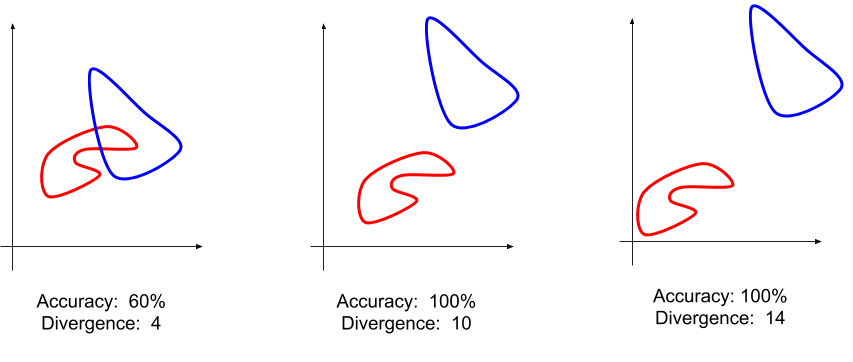
\includegraphics[width=12cm]{non_sasturating_divergence.png}
\end{center}

\subsubsection{Bhattacharyya distance}

The Bhattacharyya distance is defined on the basis of the Chernoff bound, i.e. the upper bound on the error probability of a Bayes classifier.

The Bayes classifier is an ideal classifier that has the complete knowledge of the pdf of the classes.
It works by always picking the class that minimizes the probability of error.
Thus its error probability is given by
$$ P_e = \int_{-\infty}^{+\infty} \min \left\{ \P(\omega_1) \pdf(x | \omega_1), \P(\omega_2) \pdf(x | \omega_2) \right\} \dd x $$

The direct computation of this quantity is not trivial, thus approximations are used.
Using the following relationship
$$ \min \left\{ a, b \right\} \leq a^s b^{1 - s}, \text{ where } 0 \leq s < 1 $$
we can define an upper bound $\eps_u$ for the Bayes classifier's error probability, named Chernoff bound
$$ \eps_u = \P(\omega_1)^s \P(\omega_2)^{1 - s} \int_{-\infty}^{+\infty} \pdf(x | \omega_1)^s \pdf(x | \omega_2)^{1 - s} \dd x =  \P(\omega_1)^s \P(\omega_2)^{1 - s} \exp( -\mu_{12}(s)) $$
where $\mu_{12}(s)$ is the Chernoff distance.

The choice of $s$ is not trivial, and greatly affects the result of the measure.
Instead of empirically choosing the best one, we can instead arbitrarily pick a value.
The Bhattacharyya distance is defined as the Chernoff distance with $s = 1/2$
$$ B_{i j} = \mu_{i j}(1/2) $$

As for the Divergence distance,
\begin{itemize}
    \item $i = j \implies B_{i j} = 0$
    \item $i \neq j \implies B_{i j} > 0$
    \item $B_{i j}$ is monotonically increasing with respect to the number of features, i.e. as more features are added, the discrimination increases
    \item If the features are independent, then
    $$ B_{i j}(f_1, \dots, f_k) = \sum_{q = 1}^k B_{i j}(f_q) $$
    \item Moreover, it is not saturating
\end{itemize}

The main difference from the Divergence distance is that it is related to a probability of error instead of a overlap between distributions.

\subsubsection{Jeffries-Matusita distance}
It is another distance measure with saturating behaviour.
It is defined as an average between two density functions.
$$ JM_{ij} = \left[ \int_{-\infty}^{+\infty} \left( \sqrt{\pdf(x | \omega_i)} - \sqrt{\pdf(x | \omega_j)} \right) \dd x \right]^{1/2} $$

It can be shown that the Jeffries-Matusita distance can be expressed as a function of the Bhattacharyya distance
$$ JM_{ij} = \sqrt{2 (1 - \exp(-B_{ij}))} $$


\subsection{Search strategy}
Given $n$ features with their separability measure, we want to pick the $m$ to be used in our detection.

\subsubsection{Exhaustive search}
Trying all different combinations is guaranteed to provide the optimal solution, but has prohibitive cost.
The number of combinations to be tested is given by
$$ \begin{pmatrix} n \\ m \end{pmatrix} = \frac{n!}{m! (n - m)!} $$

\subsubsection{Sequential Forward Selection}
It is a sub-optimal strategy, i.e. it is not guaranteed to give the optimal solution.
It follows a bottom-up strategy.
At every iteration, a new feature is added to the set of chosen features.
The feature to be added at each iteration is chosen as the one that most increases the separability measure of the selected features.

It is sub-optimal as it is subject to the so-called \emph{nesting effect}, i.e. a feature selected in the previous iteration can not be removed any more, even if the choice was not optimal.

\subsubsection{Sequential Backward Selection}
It is a sub-optimal strategy, similarly to SS.
It follows a top-down strategy.

Initially all the features are considered.
At every iteration, one of the considered feature is discarded.
To feature to be removed is chosen as the one that least decreases the separability measure of the selected features.

It is sub-optimal as it is subject to the so-called \emph{nesting effect}.

\subsubsection{Branch and Bound}
It is an optimal strategy, given that the separability criterion used is monotonically increasing with respect to the number of considered features.
It is a top-down strategy.

The idea is to build a hierarchical, tree-based structure that allows pruning the search space from turns that lead to non-promising solutions.
The root of the tree is the node corresponding to all the $n$ features being considered.
Given a node corresponding to $k$ features, its $k$ direct children correspond to the $k$ different solutions where one of these $k$ features is discarded.
The depth of the tree should match the number of features to discard.

Since, by hypothesis, the separability criterion is monotonically increasing with the number of considered features, we expect that if a node does not satisfy the separability requirements then also all its children will not satisfy it.
We can thus ``cut'' this branch of the tree, and avoid exploring it.


\section{Feature extraction}
Combine features instead of removing some, like in feature reduction.
The feature combination is achieved through a mapping of the sample points from an $n$-dimensional space to an $m$-dimensional one, with $m < n$.

Depending on the objective of the feature extraction, we use different methods
\begin{itemize}
    \item minimizing classification error: discriminative training
    \item minimizing reconstruction error: principal component analysis
    \item maximizing class separability: linear discriminant analysis
    \item retaining interesting directions: projection pursuit
    \item making features as independent as possible: independent component analysis
\end{itemize}

We often prefer linear mappings because they are simple to compute and are analytically tractable.
PCA and LDA are two approaches for finding optimal linear transformations.

\subsection{Principal Component Analysis}
Also called Karhunen-Loéve transform, it is an unsupervised (i.e. does not require labelled training samples) feature extraction method.
Given a set of training samples $\{\bm x_1, \dots, \bm x_N\}$, with $\bm x_i \in \mathbb R^^n$ the goal is to find a basis $\bm \phi_1, \dots, \bm \phi_m$ for an $m$-dimensional space that yields the least reconstruction error.

The criterion function for the reconstruction error can be defined in the least-squares sense as
$$ J = \sum_{i = 1}^N \norm{\sum_{k = 1}^m \bm y_{i k} \bm \phi_k - \bm x_i}^2 $$
where $\bm y_{i k}$ is the projection of $\bm x_i$ over $\bm \phi_k$

It can be shown that $J$ is minimized when $\bm \phi_1, \dots, \bm \phi_m$ are the $m$ eigenvectors of the scatter matrix $S$ having the largest eigenvalues.
The scattering matrix is defined as
$$ S = \sum_{i = 1}^N (\bm x_i - \bm m)(\bm x_i - \bm m)^T $$
where $\bm m$ is the mean of the $N$ samples.

The coefficients of each projection $\bm y_{i k}$ are called principal components


\subsection{Linear Discriminant Analysis}
It is a supervised feature extraction method.
The $n$-dimensional samples $\{\bm x_1, \dots, \bm x_N\}$ are projected on a single direction $\bm w$.
Thus, in the end, a single feature will be extracted.

Instead of minimizing the reconstruction error, it maximizes the separability.
The criterion function used is the Fisher's linear discriminant.
In the case were only 2 classes are considered
$$ J(\bm w) = \frac{\norm{\widetilde m_1 - \widetilde m_2}}{\widetilde s_1^2 + \widetilde s_2^2} $$
where $\widetilde m_i$ and $\widetilde s_i^2$ are the mean and variance of the projections of the samples belonging to the $i$-th class onto $w$.

In a geometrical interpretation, we can see that increasing $J$ means increasing the distance between the classes (numerator), or reducing their dispersion (denominator).

How to compute the optimal $\bm w$?
Let $S_i$ be the scatter matrix of the $i$-th class, i.e.
$$ S_i = \sum_{\bm x \in X_i} (\bm x - \bm m_i) (\bm x - \bm m_i)^t $$
where $X_i$ is the set of $N_i$ samples belonging to the $i$-th class and $\bm m_i = \frac{1}{N_i} \sum_{\bm x \in X_i}$ is the mean of the samples belonging to the $i$-th class.

Moreover define the within-class scatter matrix $S_W$ and the between-class scatter matrix $S_B$ as
$$ S_W = S_1 + S_2 \qquad S_B = (\bm m_1 - \bm m_2)(\bm m_1 - \bm m_2)^T $$

Then, the criterion function becomes
$$ J(\bm w) = \frac{\bm w^T S_B \bm w}{\bm w^T S_W \bm w} $$
and the optimal $\bm w$ can be computed as
$$ \bm w^{(opt)} = S_W^{-1} (\bm m_1 - \bm m_2) $$

We can generalize the LDA method to allow for more then 2 classes.
Let $C$ be the number of classes.
Then we require that $C - 1$ discriminant functions are defined, where the projection is from a $n$ dimensional space to a $(C - 1)$-dimensional space ($n \geq C$).

The within-class scatter matrix $S_W$ becomes
$$ S_W = \sum_{i = 1}^C S_i $$

and the between-class scatter matrix $S_B$ is
$$ S_B = \sum_{i = 1}^C \text{card}\{\bm X_i\} (\bm m_i - \bm m) (\bm m_i - \bm m)^t $$
where $\bm m$ is the global mean vector
$$ \bm m = \frac{1}{2} \sum_{\bm x \in \bm X} \bm x $$

The criterion function is then given by
$$ J(\bm W) = \frac{\abs{\bm W^T S_B \bm W}}{\abs{\bm W^t S_W \bm W}} $$
where $\bm W$ is the transformation matrix of size $n \times (C - 1)$ and $|\cdot|$ indicates the discriminant.

It can be shown that $J(\bm W)$ is maximized when the columns of$\bm W$ are the eigenvectors of $S_W^{-1} S_B$ having the largest eigenvalues.



\clearpage
\chapter{Supervised classification}

\section{Introduction}
Given a number of labelled samples find a partitioning of the sample space that leads the decision process.
What we can do with the given samples is
\begin{itemize}
    \item find a model of the pdf of each class
    \item gather the priors: class probabilities, costs etc
\end{itemize}

We can categorize the supervised classification approaches as follows
\begin{itemize}
    \item parametric:
    \begin{itemize}
        \item Bayesian classification
        \item MDMT, Box classifiers
    \end{itemize}

    \item Non-parametric:
    \begin{itemize}
        \item Bayesian classification
        \item kNN
        \item Neural networks
        \item Support Vector Machine
    \end{itemize}
\end{itemize}

\section{Minimum Distance To Mean classifier}
Assume that
\begin{itemize}
    \item classes have low dispersion, or
    \item classes have the same statistical behaviour (i.e. the covariance matrices are equal)
\end{itemize}

Then given an unclassified sample $x$, we can
\begin{enumerate}
    \item Compute the barycenters $m_1, \dots, m_C$ of all the classes using the labelled samples,
    \item compute the distances $d_1(x), \dots, d_C(x)$ between $x$ and the barycenters $m_1, \dots, m_C$ of all the classes,
    \item assign to $x$ the class with the closest barycenter.
\end{enumerate}

This results in a linear partitioning of the solution space, as the resulting decision boundaries will be linear.

\section{Box classifier}
In the MDMT classifier, only the 1st order statistic was used (i.e. the mean).
Moreover, the MDMT classifier is based on very restrictive assumptions.

In the box classifier, each pdf is assigned a ``box'', i.e. a hyper-cubical region in the sample space, centered at the barycenter of the class' pdf and with edges proportional to the variance of the class' pdf.

What if a sample is outside of all the boxes?
We can
\begin{itemize}
    \item label it as ``unassigned'', or
    \item apply the MDMT classifier
    \item assign it to the box with the closest boundary
\end{itemize}

\section{Bayesian classification}
Bayesian classification is a general concept, and can be divided into different categories:
\begin{itemize}
    \item full problem parametrization: the posterior probability are known exactly
    \begin{itemize}
        \item Minimum risk (MR) criterion,
        \item Maximum a posteriori (MAP) criterion, and
        \item Maximum likelihood (ML) criterion.
    \end{itemize}
    \item incomplete problem parametrization:
    \begin{itemize}
        \item Minimax criterion and
        \item Neyman-Pearson criterion.
    \end{itemize}
\end{itemize}

\subsection{Maximum a posteriori criterion}
The MAP criterion is the most commonly used one.

In the case where the class-conditional pdfs are not available, the decision criterion minimizing the error would be
$$ \widehat \omega = \argmax_{\omega_i} \{ \P(\omega_i) \}$$
i.e. we would be always choosing the class with the highest prior.
The error probability would then be
$$ P_\text{err} = 1 - \max_i \{ \P(\omega_i) \} $$

Now, assume that the posterior probabilities $\P(\omega_i | \bm x)$ are known.
Since
$$ \P(\omega_i | \bm x) = \frac{\pdf(\bm x | \omega_i) \P(\omega_i)}{\pdf(\bm x)} $$

where
\begin{itemize}
    \item the class-conditional pdf $\pdf(\bm x | \omega_i), i = 1, \dots, C$ are known, and
    \item the priors $\P(\omega_i), i = 1, \dots, C$ are known.
\end{itemize}

Then, the decision criterion that minimizes the error is the one that maximizes the posterior probability
$$ \widehat \omega = \argmax_{\omega_i} \{ \P(\omega_i | \bm x) \} = \argmax_{\omega_i} \left\{ \frac{\pdf(\bm x | \omega_i) \P(\omega_i)}{\pdf(\bm x)} \right\} $$

Since $\pdf(\bm x)$ does not depend on $\omega_i$, we can remove $\P(\bm x)$ from the above expression, obtaining the formulation of the MAP criterion
$$ \widehat \omega = \argmax_{\omega_i} \{ \pdf(\bm x | \omega_i) \P(\omega_i) \} $$
This allows to find a threshold $T$ to use for the decision.

The error probability obtained with the MAP criterion is, in the case where the samples are scalar and $C = 2$,
\begin{align*}
    P_\text{err}
    &= \P(\text{err} | \omega_1) \P(\omega_1) + \P(\text{err} | \omega_2) \P(\omega_2) \\
    &= \int_T^{+\infty} \pdf(x | \omega_1) \P(\omega_1) \dd x + \int_{-\infty}^T \pdf(x | \omega_2) \P(\omega_2) \dd x \\
    &= \int_T^{+\infty} \P(\omega_1 | x) \pdf(x) \dd x + \int_{-\infty}^T \P(\omega_2 | x) \pdf(x) \dd x & \text{for Bayes' theorem}
\end{align*}

We can also express the error as an expectation
\begin{align*}
    P_\text{err}
    &= \E{\P(\text{err} | x)} \\
    &= \int_{-\infty}^{+\infty} \P(\text{err} | x) \pdf(x) \dd x \\
    &= \int_T^{+\infty} \P(\text{err} | x) \pdf(x) \dd x + \int_{-\infty}^T \P(\text{err} | x) \pdf(x) \dd x
\end{align*}

If we compare this expression with the one found above, we can conclude that
$$ \P(\text{err} | x) = \begin{dcases}
    \P(\omega_1 | x) & \text{if } x \geq T \\
    \P(\omega_2 | x) & \text{if } x < T
\end{dcases} $$

Then, the minimum $P_\text{err}$ will be
$$ P_\text{err, min} = \int_{-\infty}^{+\infty} \min\left\{ \P(\omega_1 | x), \P(\omega_2 | x) \right\} \pdf(x) \dd x $$


\subsection{Maximum likelihood criterion}
The ML criterion is a particular case of the MAP criterion, where the priors are equal (or unknown and assumed to be equal).
Thus the priors $\P(\omega_i), i = 1, \dots, C$ are all equal and do not contribute to the decision.
The ML criterion becomes
$$ \widehat \omega = \argmax_{\omega_i} \{ \pdf(\bm x | \omega_i) \} $$

\subsection{Minimum risk criterion}
Sometimes, even though a class is less-likely to occur (i.e. has a low prior), mis-detecting it can lead to a great cost.

We can formalize this using the concept of cost matrix.
The $(i,j)$-the element $\lambda_{i,j}$ of the cost matrix $\Lambda$ is the cost incurred for taking action $\alpha_i$ for the class $\omega_j$

For example, given the classes $\omega_1 \equiv$ ``fire'' and $\omega_2 \equiv$ ``no fire'', and the actions $\alpha_1 \equiv$ ``call the firemen'' and $\alpha_2 \equiv$ ``don't call the fireman'', the cost matrix could look like follows
$$ \Lambda = \begin{pmatrix}
    0 & 500 \\
    1000000 & 0
\end{pmatrix} $$

Meaning that the cost of calling the firemen when there is no fire is not 0, but the cost of not calling the firemen where there is a fire is much higher.

Let the conditional risk $R(\alpha_i | x)$ (or expected loss) of taking an action $\alpha_i$ given the sample $x$ be
$$ R(\alpha_i | x) = \sum_{j = 1}^C \lambda(\alpha_i | x) \P(\omega_j | x) $$

The idea of the Minimum Risk criterion is that of choosing the action that minimizes the conditional risk
$$ \widehat{\alpha} = \argmin_{\alpha_i} \{ R(\alpha_i | x) \} $$

When applying the Minimum Risk criterion, then the overall risk $R^*$ is given by
$$ R^* = \int_{-\infty}^{+\infty} \min_i\{R(\alpha_i | x)\} \pdf(x) \dd x $$
and is called Bayes risk.

Let's consider the case where $x$ is scalar and $C = 2$.
Then we will decide for $\alpha_1$ if
\begin{gather*}
    R(\alpha_1 | x) \leq R(\alpha_2 | x) \\
    \lambda(\alpha_1 | \omega_1) \P(\omega_1 | x) + \lambda(\alpha_1 | \omega_2) \P(\omega_2 | x) \leq \lambda(\alpha_2 | \omega_1) \P(\omega_1 | x) + \lambda(\alpha_2 | \omega_2) \P(\omega_2 | x)
\end{gather*}

Applying the Bayes' theorem,
\begin{gather*}
        \lambda(\alpha_1 | \omega_1) \pdf(x | \omega_1) \P(\omega_1) + \lambda(\alpha_1 | \omega_2) \pdf(x | \omega_2) \P(\omega_2) \leq \lambda(\alpha_2 | \omega_1) \pdf(x | \omega_1) \P(\omega_1) + \lambda(\alpha_2 | \omega_2) \pdf(x | \omega_2) \P(\omega_2) \\
        \pdf(x | \omega_1) [\lambda(\alpha_1 | \omega_1) - \lambda(\alpha_2 | \omega_1)] \P(\omega_1) \leq \pdf(x | \omega_2) [\lambda(\alpha_2 | \omega_2) - \lambda(\alpha_1 | \omega_2)] \P(\omega_2)
\end{gather*}

In general, $\lambda(\alpha_1|\omega_1) < \lambda(\alpha_2|\omega_1)$ and $\lambda(\alpha_2|\omega_2) < \lambda(\alpha_1|\omega_2)$, thus
$$  \pdf(x | \omega_1) \underbrace{[\lambda(\alpha_1 | \omega_1) - \lambda(\alpha_2 | \omega_1)]}_{< 0} \P(\omega_1) \leq \pdf(x | \omega_2) [\lambda(\alpha_2 | \omega_2) - \lambda(\alpha_1 | \omega_2)] \P(\omega_2) $$

We'll move this quantity to the right, but since it is negative we must change the sign of the equation from $\leq$ to $\geq$
$$ \frac{\pdf(x | \omega_1)}{\pdf(x | \omega_2)} \geq \underbrace{\frac{\lambda(\alpha_2 | \omega_2) - \lambda(\alpha_1 | \omega_2)}{\lambda(\alpha_1 | \omega_1) - \lambda(\alpha_2 | \omega_1)} \frac{\P(\omega_2)}{\P(\omega_1)}}_\eta $$
where $\eta$ can be seen as a sort of a threshold.

Moreover,
\begin{itemize}
    \item if $\lambda(\alpha_1|\omega_1) = \lambda(\alpha_2|\omega_2) = 0$ then
    $$ \eta = \frac{\lambda(\alpha_1 | \omega_2)}{\lambda(\alpha_2 | \omega_1)} \frac{\P(\omega_2)}{\P(\omega_1)} $$

    \item if the costs are the same for the two classes, then
    $$ \eta = \frac{\P(\omega_2)}{\P(\omega_1)} $$
    and we obtain the MAP criterion.

    \item if the priors are equal, i.e. $\P(\omega_2) = \P(\omega_1)$, then
    $$ \eta = 1 $$
    and we obtain the ML criterion.
\end{itemize}


\subsection{Discriminant functions}
The sample $\bm x$ is assigned to the class $\widehat \omega$ such that
$$ \widehat \omega = \argmax_{\omega_i} \{ g_{\omega_i}(\bm x) \} $$
where $g_{\omega_1}, \dots, g_{\omega_C}$ are the so-called discriminant functions.

The discriminant functions can be chosen freely.
For example,
\begin{itemize}
    \item by choosing $g_{\omega_i} = -R(\alpha_i, x)$, the MR criterion is obtained,
    \item by choosing $g_{\omega_i} = \P(\omega_i | \bm x)$, the MAP criterion is obtained,
    \item by choosing $g_{\omega_i} = \pdf(\bm x | \omega_i)$ the ML criterion is obtained.
\end{itemize}

Assume that the sample space is $n$-dimensional, and that the pdf of the $C$ classes considered are multi-variate gaussians, i.e.
$$ \pdf(\bm x | \omega_i) = N(\bm m_i, \bm \Sigma_i) = \frac{1}{\sqrt{(2 \pi)^n \abs{\bm \Sigma_i}}} \exp(-\frac{1}{2} (\bm x - \bm \mu_i)^T \bm \Sigma_i^{-1} (\bm x - \bm \mu_i)) $$

Consider the MAP criterion as implemented with discriminant functions.
To simplify the computation, we will consider the logarithms $g_i$ of the posterior probabilities
\begin{align*}
    g_i(\bm x)
    &\triangleq \ln(\P(\omega_i | \bm x)) \\
    &= \ln(\pdf(\bm x | \omega_i)) + \ln(\P(\omega_i)) & \text{for Bayes' theorem} \\
    &= -\frac{1}{2} (\bm x - \bm m_i)^T \bm \Sigma_i^{-1} (\bm x - \bm m_i) - \underbrace{\frac{n}{2} \ln(2 \pi)}_{\substack{\text{does not} \\ \text{depend on } i}} - \frac{1}{2} \ln(\abs{\bm \Sigma_i}) + \ln(\P(\omega_i))
\end{align*}
where $\abs{\bm \Sigma_i}$ indicates the determinant of the $\bm \Sigma_i$ matrix.

We can disregard the term not depending on $i$, as it will not contribute to the decision process, obtaining
\begin{align*}
    g_i(\bm x)
    &= -\frac{1}{2} (\bm x - \bm m_i)^T \bm \Sigma_i^{-1} (\bm x - \bm m_i) - \frac{1}{2} \ln(\abs{\bm \Sigma_i}) + \ln(\P(\omega_i)) \\
    &= -\frac{1}{2} \left[ \bm x^T \bm \Sigma_i^{-1} \bm x - 2 \bm m_i^T \bm \Sigma_i^{-1} \bm x + \bm m_i^T \bm \Sigma_i^{-1} \bm m_i \right] - \frac{1}{2} \ln(\abs{\bm \Sigma_i}) + \ln(\P(\omega_i))
\end{align*}

This function combines the features quadratically.
We can study some particular cases:
\begin{itemize}
    \item
    If the features are completely independent, then the covariance matrices $\bm \Sigma_i$ are diagonal, and, if they are also equal for all the classes ($\bm \Sigma_i \equiv \bm \Sigma$)
    $$ \bm \Sigma = \sigma^2 \bm I \quad \text{and} \quad \bm \Sigma^{-1} = \frac{1}{\sigma^2} \bm I \quad \text{and} \quad \abs{\bm \Sigma} = \sigma^{2 n} $$

    Then
    $$ g_i(\bm x)
    =
    \underbrace{-\frac{1}{2 \sigma^2} \norm{\bm x}}_{\substack{\text{does not} \\ \text{depend on } i}}
    + \frac{1}{\sigma^2} \bm m_i^T
    - \underbrace{\frac{1}{2} \ln(\sigma^{2 n})}_{\substack{\text{does not} \\ \text{depend on } i}}
    - \frac{1}{2} \frac{\norm{\bm m_i}^2}{\sigma^2}
    + \ln(\P(\omega_i)) $$

    Further removing the terms that do not depend on $i$ yields
    $$ g_i(\bm x) = \bm w_i^T \bm x + \text{bias}_i $$
    where
    $$ \bm w_i = \frac{1}{\sigma^2} \bm m_i \quad \text{and} \quad \text{bias}_i = \ln(\P(\omega_i)) - \frac{1}{2 \sigma^2} \norm{\bm m_i}^2 $$

    The discriminant function is thus linear with respect to $\bm x$!
    The decision boundary between the $i$-th and $j$-th classes will then be located at
    \begin{gather*}
        g_i(\bm x) = g_j(\bm x) \\
        \bm w_i^T \bm x + \text{bias}_i = \bm w_j^T \bm x + \text{bias}_j \\
        \bm w^T (\bm x - \bm x_0) = 0 \quad \text{where} \quad \begin{dcases}
            \bm w = \bm w_i - \bm w_j \\
            \bm x_0 = \frac{1}{2} (\bm m_i + \bm m_j) + \frac{\sigma^2}{\norm{\bm m_i - \bm m_j}^2} \ln(\frac{\P(\omega_i)}{\P(\omega_j)}) (\bm m_i - \bm m_j)
        \end{dcases}
    \end{gather*}

    The decision boundary between the $i$-th and $j$-th classes is a hyperplane that passes through $\bm x_0$ and is orthogonal to $\bm w$.

    In the case where the priors are the same, we get a result very similar to that obtained with the MDTM classifier.

    \item
    Consider the case where covariance matrices of the different classes are all equal ($\bm \Sigma_i \equiv \bm \Sigma$), but not necessarily diagonal.

    Then
    $$ g_i(\bm x) =
        \underbrace{-\frac{1}{2} \bm x^T \bm \Sigma^{-1} \bm x}_{\substack{\text{does not} \\ \text{depend on } i}}
        + \bm m_i^T \bm \Sigma^{-1} \bm x
        - \frac{1}{2} \bm m_i^T \bm \Sigma^{-1} \bm m_i
        - \underbrace{\frac{1}{2} \ln(\abs{\bm \Sigma})}_{\substack{\text{does not} \\ \text{depend on } i}}
        + \ln(\P(\omega_i)) $$
    Removing the terms that do not depend on $i$
    \begin{align*}
        g_i(\bm x)
        &= \bm m_i^T \bm \Sigma^{-1} \bm x - \frac{1}{2} \bm m_i^T \bm \Sigma^{-1} \bm m_i + \ln(\P(\omega_i)) \\
        &= (\bm \Sigma^{-1} \bm m_i)^{-1} \bm x - \frac{1}{2} \bm m_i^T \bm \Sigma^{-1} \bm m_i + \ln(\P(\omega_i)) \\
        &= \bm w_i^T \bm x + \text{bias}_i
    \end{align*}

    where
    $$ \bm w_i = \bm \Sigma^{-1} \bm m_i \quad \text{ and } \quad \text{bias}_i = \ln(\P(\omega_i)) - \frac{1}{2} \bm m_i^T \bm \Sigma^{-1} \bm m_i $$

    Again, the discriminant function is linear with respect to $\bm x$.
    As a consequence, the decision boundary will again be linear, but it won't be perpendicular to the $\bm m_i - \bm m_j$, but instead will be rotated.

    The decision boundary between the $i$-th and $j$-th classes satisfies
    $$ \bm w^T (\bm x - \bm x_0) = 0 \qquad \text{where} \quad \begin{dcases}
        \bm w = \overbrace{\bm \Sigma^{-1}}^{\substack{\text{modulates the $\bm m_i - \bm m_j$ direction } \\ \text{based on the pdfs characteristics}}} (\bm m_i - \bm m_j) \\
        \bm x_0 = \frac{1}{2} (\bm m_i + \bm m_j) - \ln(\frac{\P(\omega_i)}{\P(\omega_j)}) \frac{\bm m_i - \bm m_j}{(\bm m_i - \bm m_j)^T \bm \Sigma^{-1} (\bm m_i - \bm m_j)}
    \end{dcases} $$

    \vskip1cm

    \begin{center}
        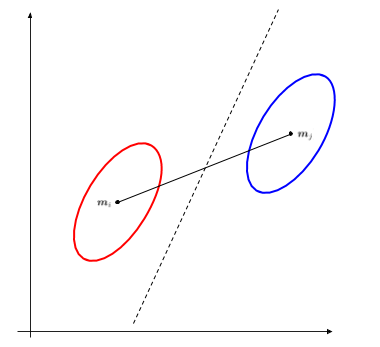
\includegraphics[width=8cm]{discriminant_function_classification.png}
    \end{center}

    \item
    In the case where the different covariance matrices $\bm \Sigma_i$ are all different, the criterion function is a quadratic function of $\bm x$.
    In that case the boundaries will be hyper-quadratic, i.e.
    \begin{itemize}
        \item parallel lines
        \item parables
        \item ellipses
        \item nested ellipses
        \item hyperboles
        \item crossing lines
    \end{itemize}
\end{itemize}


\subsection{Supervised signal detection theory}
This section reports the supervised signal detection theory developed by the radar researchers in the past decades.
The problem of signal detection in radar application can be seen as a binary classification problem, where we have to pick one of two hypothesis:
\begin{itemize}
    \item $H_0$: no signal, target absent, and
    \item $H_1$: signal detected, target present.
\end{itemize}
To shorten the notation, we often use $P_0 = \P(H_0)$ and $P_1 = \P(H_1)$.

The choice should be performed based on $n$ features $\bm x$.
Let $Z_0$ and $Z_1$ be the decision regions of $H_0$ and $H_1$.
The class conditional pdfs $\pdf(\bm x | \omega_1)$ and $\pdf(\bm x | \omega_2)$ are assumed to be known.

\subsection{Minimum risk criterion}
Let $D_0$ and $D_1$ be the decisions for ``target absent'' and ``target present'', respectively.

We define the following costs $c_{00}, c_{01}, c_{10}, c_{11}$ as
$$ c_{i j} \equiv \text{``the cost of deciding } D_i \text{ when actually it is } H_j \text{''} $$

In general, $c_{10} > c_{00}$ and $c_{01} > c_{11}$.

Moreover, we define the following probabilities
\begin{itemize}
    \item the probability of correct rejection, $P_\text{CR} = P(D_0 | H_0)$
    \item the probability of false alarm, $P_\text{FA} = P(D_1 | H_0)$
    \item the probability of missed alarm, $P_\text{MA} = P(D_0 | H_1)$
    \item the probability of correct detection, $P_\text{D} = P(D_1 | H_1)$
\end{itemize}

Note that
\begin{itemize}
    \item $P_\text{CR} + P_\text{FA} = 1$
    \item $P_\text{MA} + P_\text{D} = 1$
\end{itemize}

The average cost is given by
\begin{align*}
    R
    &= \E{\text{cost}} \\
    &= c_{00} \P(D_0, H_0) + c_{10} \P(D_1, H_0) + c_{01} \P(D_0, H_1) + c_{11} \P(D_1, H_1) \\
    &= c_{00} \P(D_0 | H_0) \P(H_0) + c_{10} \P(D_1 | H_0) \P(H_0) \\
    &\quad + c_{01} \P(D_0 | H_1) \P(H_1) + c_{11} \P(D_1 | H_1) \P(H_1) & \text{for the definition of conditional probability} \\
    &= c_{00} P_\text{CR} P_0 + c_{10} P_\text{FA} P_0 + c_{01} P_\text{MD} P_1 + c_{11} P_\text{D} P_1 \\
    &= c_{00} (1 - P_\text{FA}) P_0 + c_{10} P_\text{FA} P_0 + c_{01} (1 - P_\text{D}) P_1 + c_{11} P_\text{D} P_1 \\
    &= \underbrace{c_{00} P_0 + c_{01} P_1}_\text{constants w.r.t. $Z_1$} - c_{00} P_\text{FA} P_0 + c_{10} P_\text{FA} P_0 - c_{01} P_\text{D} P_1 + c_{11} P_\text{D} P_1 \\
    &= \text{const} + P_0 (c_{10} - c_{00}) P_\text{FA} - P_1 (c_{01} - c_{11}) P_\text{D} \\
    &= \text{const} + \int_{Z_1} [ \underbrace{P_0 (c_{10} - c_{00}) \pdf(x | H_0)}_{\geq 0} - \underbrace{P_1 (c_{01} - c_{11}) \pdf(x | H_1)}_{\geq 0} ] \dd x
\end{align*}

To minimize $R$, we should find $Z_1$ so that the sum in the first term in the integral be less than the second term in the integral.
This yields
$$ \underbrace{\frac{\pdf(x | H_1)}{\pdf(x | H_0)}}_\text{likelihood ratio} > \underbrace{\frac{P_0 (c_{10} - c_{00})}{P_1 (c_{01} - c_{11})}}_\eta $$

If this holds true, $x$ will be assigned to $Z_1$.

When discussing the Minimum risk criterion previously, we started from a point to find the decision region using the criterion (bottom up strategy). This time, we started from the global perspective i.e. from the expression for the average risk (top down).


\subsection{Minimax criterion}
The MR criterion is the optimal decision criterion when the priors and the class-conditional pdfs are known.
But what if the priors are not known?
In this case we can reason in terms of worst case scenarios, i.e. we behave as if the priors assumed the probability values that lead to the maximum minimum risk.

Let's consider the case where the priors $P_1$ and $P_0$ corresponding to ``target present'' and ``target not present'' are not known.
We can express the threshold $\eta$ used in the MR criterion as a function of $P_1$, also remembering that $P_0 = 1 - P_1$ as follows
$$ \eta(P_1) = \frac{1 - P_1}{P_1} \frac{c_{10} - c_{00}}{c_{01} - c_{11}} $$

Once $\eta(P_1)$ is known, the decision regions $Z_0$ and $Z_1$ can also be defined.
Thus, the probability of false alarm $P_F$ and the probability of missed detection $P_M$ only depend on $P_1$.
$$ P_F = \P(D_1 | H_0) = \int_{Z_1} \pdf(x | H_0) \dd x \qquad
P_M = \P(D_0 | H_1) = \int_{Z_0} \pdf(x | H_1) \dd x $$

Finally, the average risk $R(P_1)$ associated to the prior $P_1$ is given by
$$ R(P_1) =
c_{00} (1 - P_F(P_1)) (1 - P_1) +
c_{10} P_F(P_1) (1 - P_1) +
c_{01} P_M(P_1) P_1 +
c_{11} (1 - P_M(P_1)) P_1
$$

Which is generally a quadratic function of $P_1$.
\begin{center}
    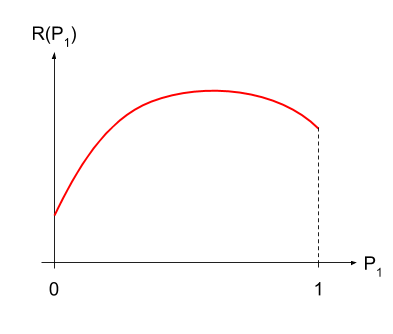
\includegraphics[width=8cm]{minimum_risk_vs_p1.png}
\end{center}

However, computation of $P_F(P_1)$ and $P_M(P_1)$ for all the possible $P_1$ values is computationally demanding, as they require the evaluation of the integral of the class-conditional probabilities.
Thus, computing $R(P_1)$ exactly is not feasible.

Instead, we can compute $P_F(P_1)$ and $P_M(P_1)$ for a single, arbitrary value $P_1^*$ as
$$ P_F^* = P_F(P_1^*) \qquad P_M^* = P_M(P_1^*) $$

Now, if $P_F^*$ and $P_M^*$ are plugged in the risk computation in place of  $P_F(P_1)$ and $P_M(P_1)$, the risk $R^*(P_1)$ is obtained
\begin{align*}
    R^*(P_1)
    &= c_{00} (1 - P_F^*) (1 - P_1) +
    c_{10} P_F^* (1 - P_1) +
    c_{01} P_M^* P_1 +
    c_{11} (1 - P_M^*) P_1 \\
    &= c_{00} (1 - P_F^*) + c_{10} P_F^* + P_1 \left[ c_{11} - c_{00} + (c_{00} - c_{10}) P_F^* + (c_{01} - c_{11}) P_M^* \right]
\end{align*}

The risk $R^*(P_1)$ computed in this way is not the optimal risk, thus $R^*(P_1) \geq R(P_1)$.
Instead, $R^*(P_1) = R(P_1)$ only for $P_1 = P_1^*$.
Moreover, we can notice that $R^*(P_1)$ is a linear function of $P_1$.
As a result of these considerations, we expect $R^*(P_1)$ to be a line that is tangential to the minimal risk quadratic curve $R(P_1)$ in the point $P_1^*$.
\begin{center}
    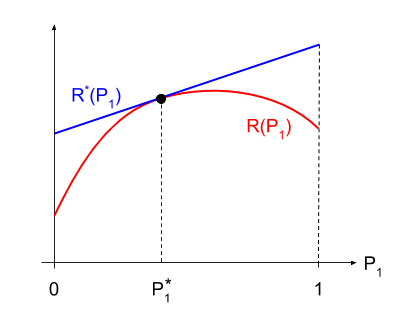
\includegraphics[width=8cm]{approx_minimum_risk_vs_p1.png}
\end{center}

Let's consider the situation when
$$ P_1^* = \argmax_{P_1 \in[0, 1]}\{R(P_1)\} $$

If $P_1^*$ is the maximum of $R(P_1)$, then its derivative in that point is 0.
As noted before, $R^*(P_1)$ is the line tangential to the quadratic function $R(P_1)$, and thus it's slope is equal to the derivative of $R(P_1)$.

Vice versa, if we can find the value of $P_1^*$ that makes $R^*(P_1)$ horizontal, this means that $P_1^*$ is the maximum of $R(P_1)$, i.e. what we where looking for.
$R^*(P_1)$ is horizontal if it's derivative is zero, thus
\begin{gather*}
    \pdv{R^*(P_1)}{P_1} = 0 \\
    c_{11} - c_{00} + (c_{00} - c_{10}) P_F^* + (c_{01} - c_{11}) P_M^* = 0
\end{gather*}

In the case where $c_{11} = c_{00} = 0$ and $c_{10} = c_{01}$, then the minimax condition becomes
\begin{align*}
    &P_1: P_F^* = P_M^* \\
    &P_1: P_F(P_1^*) = P_M(P_1^*) \\
    &P_1: P_F(P_1^*) = 1 - P_D(P_1^*) \\
    &P_1: \int_{Z_0} \pdf(x | H_0) \dd x = 1 - \int_{Z_0} \pdf(x | H_1) \dd x \\
    &P_1: \int_{Z_0} [ \pdf(x | H_0) + \pdf(x | H_1)] \dd x = 1
\end{align*}

In this case, the decision region $Z_0$ obtained with the minimax criterion is the one making the integral of the sum of the class conditional pdfs 1.


\subsection{Neyman-Pearson Criterion}
Another case in which the MR criterion can't be applied is when we want to embed additional constraints in the decision process.
Assume that only the class-conditional models are known, and we want to minimize $P_M$ (or $P_F$) under the constraint that $P_F$ (or $P_M$) should be below a given threshold value $\alpha$.
If neither the priors nor the costs are known, the Neyman-Pearson criterion can be applied.

The problem can set as a constrained optimization problem
\begin{gather}
    \text{Find } \argmin_{Z_0}\left\{ P_M = \int_{Z_0} \pdf(x | H_1) \dd x \right\} \\
    \text{subject to } P_F = \int_{Z_1} \pdf(x | H_0) \dd x = \alpha
\end{gather}

To solve constrained optimization problems, we can use the lagrangian multipliers method.
We introduce a new variable, the lagrangian multiplier $\lambda$ and study the following Lagrange function $\mathcal L(Z_0, \lambda)$
\begin{align*}
    \mathcal L(Z_0, \lambda)
    &= P_M + \lambda (P_F - \alpha) \\
    &= P_M + \lambda (1 - P_{CR} - \alpha) \\
    &= \int_{Z_0} \pdf(x | H_1) \dd x + \lambda \left(1 - \int_{Z_0} \pdf(x | H_0) \dd x - \alpha \right) \\
    &= \int_{Z_0} \pdf(x | H_1) \dd x - \lambda \left( \int_{Z_0} \pdf(x | H_0) \dd x \right) + \lambda \left(1 - \alpha \right) \\
    &= \int_{Z_0} \Big[ \underbrace{\pdf(x | H_1)}_{\geq 0} - \underbrace{\lambda \pdf(x | H_0)}_{\geq 0} \Big] \dd x + \lambda \left(1 - \alpha \right)
% Why do we assume that \lamdba \geq 0?
\end{align*}

% Why can we disregard the rigth term?? Maybe because it is the only part depending on Z_0


Let's consider the integral in the equation above.
The integral is minimized when
$$ \pdf(x | H_1) < \lambda \pdf(x | H_0) \quad \forall x \in Z_0 $$

We can rephrase this as a condition on $Z_0$
\begin{align*}
    Z_0
    &= \left\{ x : \pdf(x | H_1) < \lambda \pdf(x | H_0) \right\} \\
    &= \Big\{ x : \underbrace{\frac{\pdf(x | H_1)}{\pdf(x | H_0)}}_{\substack{\text{Likelihood} \\ \text{ratio, } \Lambda(x) }} < \lambda \Big\}
\end{align*}

We have now found $Z_0$ as a function of $\lambda$.
We can now find $\lambda$ itself by using the constraint
\begin{gather*}
    P_F = \alpha \\
    \P(\Lambda(x) > \lambda | H_0) = \alpha \\
    \int_\lambda^{+\infty} \pdf(\Lambda(x) | H_0) \dd x = \alpha
\end{gather*}
But since $\Lambda(x)$ does not depend on $H_0$,
$$ \int_\lambda^{+\infty} \pdf(\Lambda(x)) \dd x = \alpha $$

In general, it is not possible to find an analytical solution to the above expression.
If that is the case, the threshold $\lambda$ must be found numerically.


\subsection{The Receiver Operating Characteristic}
The ROC curve captures the behaviour of the detection probability $P_D$ as a function of the false alarm probability $P_F$ for a fixed value of the decision threshold.

The ROC curve always passes through the points $(0, 0)$ and $(1, 1)$, since
\begin{itemize}
    \item $Z_1 = \varnothing \implies P_D \to 0, P_F \to 0$
    \item $Z_0 = \varnothing \implies P_D \to 1, P_F \to 1$
\end{itemize}


In the left of the following figure, a number of different threshold values are reported for a given two-class decision problem.
The corresponding ROC values obtained with each of the different threshold values are shown on the right.
\begin{center}
    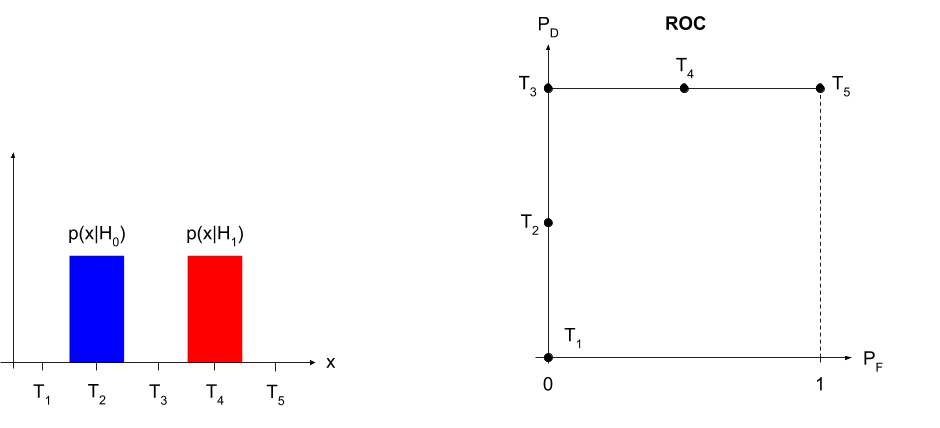
\includegraphics[width=12cm]{roc_curve_example.png}
\end{center}

In the above case, the classes were completely separated, and the resulting ROC curve was rectangular.
Let's consider the opposite case, i.e. when the classes are completely overlapping.
In that case, the ROC curve will correspond to the bisector of the first quadrant.
\begin{center}
    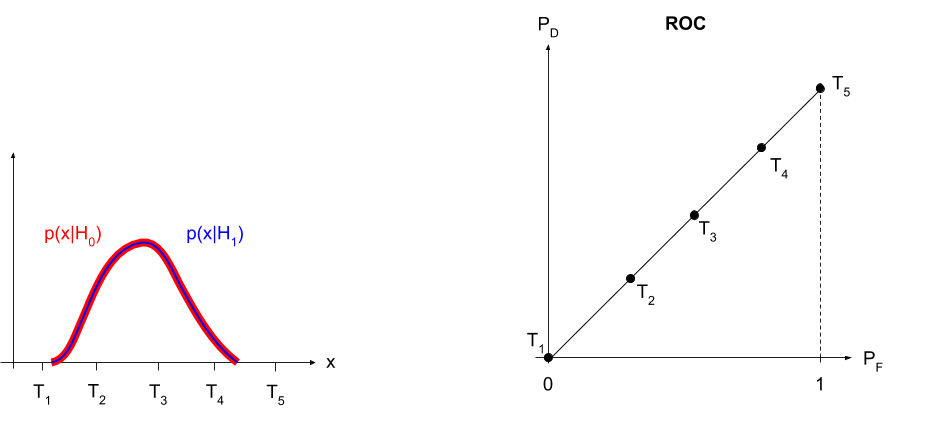
\includegraphics[width=12cm]{roc_curve_overlapping.png}
\end{center}

Thus, by looking at the ROC curve (and assuming the receiver has been designed well), we can understand how separable the classes of a given problem are, and how hard the problem is.

When the classes considered are gaussians, the ROC curve can be parametrized in terms of their ``distance''.

It can be shown that:
\begin{itemize}
    \item The slope of the tangent to the ROC curve is equal to the value of $\eta$ for which $P_F$ and $P_D$ correspond (i.e. the threshold used in the MR criterion).
    \item The $P_D$ corresponding to a given $P_F$ is the ordinate yielded by the NP criterion, when imposing $P_F = \alpha$.
    \item Every point $(P_F, P_D)$ of the ROC curve is the intersection between the ROC curve and the minimax line, as shown next
    \begin{gather*}
        c_{11} - c_{00} + (c_{00} - c_{10}) P_F + (c_{01} - c_{11}) P_M = 0 \\
        c_{11} - c_{00} + (c_{01} - c_{11}) P_M = (c_{10} - c_{00}) P_F \\
        c_{11} - c_{00} + (c_{01} - c_{11}) (1 - P_D) = (c_{10} - c_{00}) P_F \\
        \cancel{c_{11}} - c_{00} + c_{01} - \cancel{c_{11}} + (c_{11} - c_{01}) P_D = (c_{10} - c_{00}) P_F \\
        P_D = \underbrace{\frac{c_{10} - c_{00}}{c_{11} - c_{01}}}_{< 0} P_F + \frac{c_{00} - c_{01}}{c_{11} - c_{01}}
    \end{gather*}
\end{itemize}



\section{Classifier fusion}
Different classifiers might be best in different parts of the feature space.
Thus is might be convenient to perform classifier fusion, where two or more classifiers are combined in parallel and their output combined.


\subsection{Classifier combination}
Typical combination scenario are the following 3.

\paragraph{Traditional classification}
All classifiers work on the same feature space, but are designed so that their errors are as uncorrelated as possible.
To achieve this, they can differ
\begin{itemize}
    \item in the methodologies used,
    \item in the architecture or parameters used, or
    \item in the manipulation over their training set:
    \begin{itemize}
        \item noise injection: independent noise sources are combined with the training samples of each classifier
        \item bagging: group the original training sample set in different bags, each is used to train a different classifier
        \item boosting: the training samples misclassified by the first classifier are used to form a second version of the training set, which is then used to train a second classifier.
        The misclassified samples can be weighted based on the confidence/posterior probability output by the first classifier, so that more important mistakes are fixed.
    \end{itemize}
\end{itemize}

\paragraph{Multisensor/mutlisource classification}
Each classifier is fed by a different source of information.
This allows for different methodologies to be used for different information sources, and to avoid a high number of input features.
However, the information sources must not be correlated.

\paragraph{Hyperdimensional classification}
Each classifier is defined over a subset of the available features.
For example, when the input data is the EM radiation, we could have more classifiers working on different portions of the spectrum (e.g. infrared, visible, ultra-violet).
Attacking the problem with a higher number of classifiers has the advantage of incurring in a less acute Huge effect.
However, it also decomposes the global classification problem into a more local one, and thus could lead to lower accuracy, do to some missed correlations.


\subsection{Fusion architectures}
The fusion architecture can be
\begin{itemize}
    \item Parallel architecture: the classifiers are all run in parallel and their outputs combined by means of an appropriate fusion strategy

    \item Cascade architecture: classifiers are run in cascade.
    Each classifier is devoted to detecting a specific class.
    If a classifiers does not consider a sample to belong to its related class, the baton is passed to the next classifier in the cascade.

    \item Hybrid architecture: a mix of the above two architectures.
\end{itemize}


\subsection{Fusion strategies for parallel architecture}
The most important part of a parallel classifier fusion is choosing how to combine the outputs of different classifiers, also referred to fusion strategy.

There are three main categories of classifiers fusion
\begin{itemize}
    \item decision fusion: only the decisions are considered (e.g. Majority vote)
    \item unsupervised posterior probability fusion: the confidence of each classifier is taken into consideration (e.g. Averaging)
    \item supervised posterior probability fusion: like the previous one, but requires the use of labelled training samples (e.g. Weighted averaging)
\end{itemize}

\paragraph{Majority vote}
Assign the label that most of the classifiers in the ensemble assign.
More specifically, the rule can rely on
\begin{itemize}
    \item Unanimity: only label if all classifiers agree on the label
    \item Simple majority: choose the label that at least 50\% of the classifiers assigned
    \item plurality: assign the most voted label
\end{itemize}
The number of classifiers should clearly been odd to avoid ties.

In the hypothesis that all the $Q$ classifiers have the same probability $p$ of making the correct decisions and are independent, the probability $P$ to perform the correct decision based on the simple majority follows the Bernoulli distribution.
It can be easily shown that
$$ \lim_{Q \to +\infty} P = \begin{dcases}
    1 & \text{if } p > 0.5 \\
    1/2 & \text{if } p = 0.5 \\
    0 & \text{if } p < 0.5
\end{dcases} $$

\paragraph{Averaging}
The posterior probabilities are seen as estimates of the posterior probabilities.
The decision rule is based on the MAP criterion applied on the averaged posteriors.

In practical terms, we decide for the class that maximises the average confidence of all the classifiers
$$ \widehat w = \argmax_{k = 1,\dots,C} \left\{ \sum_{j = 1}^Q P_j(\omega_k | \bm x) \right\} $$

\paragraph{Weighted Averaging}
The Averaging fusion strategy assumes that all the classifiers have the same accuracy.
Instead, we can weight each classifier's estimate with a specific weight.

\begin{center}
    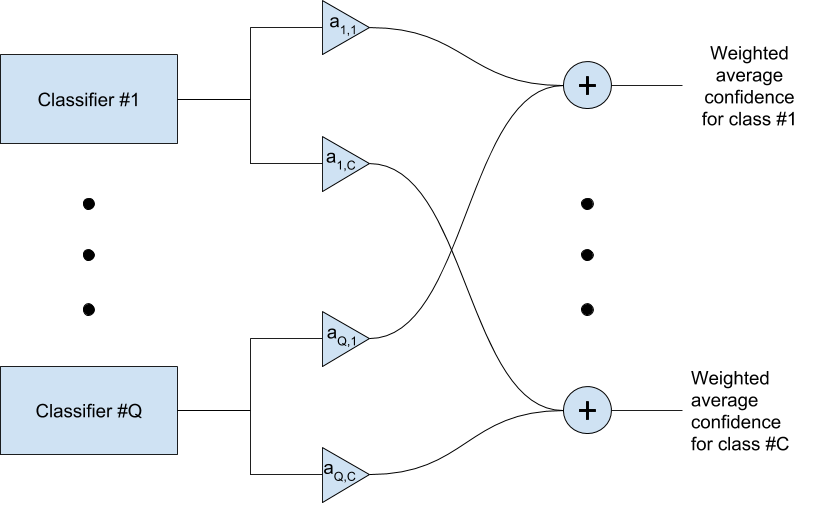
\includegraphics[width=10cm]{weighted_averaging_fusion_strategy.png}
\end{center}

The weights of the classifiers can be found by considering the confidence of each classifier output for a set of validation samples, and later computing the weights using the pseudo-inverse matrix to minimize the mean square error.

If we represent the weights in matrix forms, then
$$ \underline{\underline{A}} = \left[ \underline a_1, \dots, \underline a_C \right] \qquad \text{ where } \underline a_j = \left[ a_{1, j}, \dots, a_{Q, j} \right]^T $$

Assume that $N$ validation samples.
For each sample $i$ and each class $j$, we compute the desired target output as
$$ T_{i, j} = \begin{dcases}
    1 & \text{if the $i$-the sample belongs to the $j$-th class} \\
    0 & \text{otherwise}
\end{dcases} $$

Then we set up the problem of finding the weights $\underline a_j$ for the $j$-th class in matrix form as follows
\begin{gather*}
    \begin{bmatrix}
        P_1(\omega_j | x_1) & \dots & P_Q(\omega_j | x_1) \\
        \vdots &  & \vdots \\
        P_1(\omega_j | x_N) & \dots & P_Q(\omega_j | x_N)
    \end{bmatrix}
    \begin{bmatrix}
        a_{1, j} \\
        \vdots \\
        a_{Q, j}
    \end{bmatrix}
    =
    \begin{bmatrix}
        T_{1, j} \\
        \vdots \\
        T_{Q, j}
    \end{bmatrix} \\
    \underline{\underline{P_j}}
    \ \underline{a_j}
    =
    \underline{T_j}
\end{gather*}

Using the pseudo-matrix inversion, the solution in the least square sense can be found as
$$ \underline{a_j} = \left( \underline{\underline{P_j}}^T \underline{\underline{P_j}} \right)^{-1} \underline{\underline{P_j}} \ \underline{T_j} $$




\section{Contextual classification with Markov Random Fields}
\subsection{Introduction}
Until now we assumed that the decision for a given sample does not depend on its context.
How can we include the context information in the decision process?
\begin{itemize}
    \item At a preprocessing level
    \item At the decision level: with Markov Random Fields
\end{itemize}

Let $\Omega = \{\omega_i, i = 1, \dots, c\}$ be the classes that can be assigned to each of the pixels of a given image $I$ of size $K \times J$.
Let $\bm C$ be the set of all the possible classification maps, thus $\text{card}\{\bm C\} = c^{K J}$.
Let $C_i$ be any the possible classification maps in $\bm C$.

Suppose we want to assign a class to each of the pixels of an image $I$.
The MAP decision rule for the whole image is
$$ \widehat C = \argmax_{C_i \in \bm C}\{\P(C_i | I)\} = \argmax_{C_i \in \bm C}\{\pdf(I | C_i) \P(C_i) \} $$
But $\pdf(I | C_i)$ and $\P(C_i)$ are hard to compute.
We'll introduce two assumptions that will simplify the mathematical formulation:
\begin{itemize}
    \item the spatial contextual information will be modelled locally
    \item class-conditional independence: i.e. the class-conditional distribution of each pixel is independent of other pixels, and thus the map-conditional distribution of the whole image can be computed as a product of the class-conditional distribution of each pixel.
    $$ \pdf(I | C_i) = \prod_{I(j, k) \in I} \pdf(I(j, k) | C_i(j, k)) $$
\end{itemize}

\subsection{Markov Random Fields and Energy}
A random field is a collection of random variables indexed in a particular topological space (in our case, a 2D grid).
A random field is said to be a Markov Random Field (MRF) with respect to a given neighbourhood system $N$, if the related probability function satisfies the following properties:
\begin{itemize}
    \item positivity:
    $$ P(C_i) > 0 \quad \forall C_i \in C $$
    meaning that every possible map is associated to a non-zero probability.

    \item Markov property: the class distribution of a specific pixel is independent from the classes of the pixels that do not belong to its neighbourhood
    $$ P\Big(C_i(j, k) \Big| \big\{ C_i(g, h), \forall (g, h) \neq (j, k) \big\}\Big) =
    P\Big(C_i(j, k) \Big| \big\{ C_i(g, h), \forall (g, h) \in N(j, k) \big\}\Big) $$

    \item Homogeneity or spatial stationarity: the class distribution of all the pixels, conditioned to the classes of their neighbour pixels, follow the same distribution.
\end{itemize}

A neighbour system depends on the order of the spatial dependencies.
First and second order neighbourhood systems are the most commonly used.

\begin{center}
    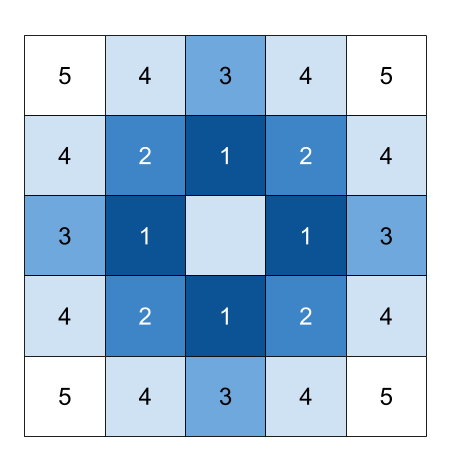
\includegraphics[width=5cm]{neighbourhood_system.png}
\end{center}

A clique is an elementary structure which expresses the local spatial relationships between pixels. The set of all cliques defines completely the considered neighbourhood system.

A potential function $V_q(C_i)$ defines the energy associated with a given clique $q$ of the neighbourhood system $N$.
The total energy function in $N$ is given by
$$ U(C_i) = \sum_{q \in N} V_q(C_i) $$

A Gibbs Random Field (GRF) is a random field for which the global prior model is expressed in terms of the energy functions as follows
$$ P(C_i) = \frac{1}{Z} \exp(-U(C_i)) $$
where $Z$ is a normalization constant.

The Hammersley-Clifford theorem states that, given a neighbourhood system $N$, $C_i$ is a MRF with respect to $N$ if and only if $P(C_l)$ follows a Gibbs distribution with respect to $N$.

Thus, if a random field is a MRF with respect to $N$, it is possible to define a global model from the local characteristics of the image (which contains most of the spatial correlation) by means of the Gibbs distribution.

If a random field is a MRF with respect to $N$, then
$$ \P\Big(C_i(j, k) \Big| \big\{ C_i(g, h), \forall (g, h) \neq (j, k) \big\} \Big) = \frac{1}{Z} \exp(-U \left( C_i(j, k) \Big| \big\{ C_i(g, h), \forall (g, h) \in N(j, k) \big\} \right)) $$

A simple formulation of the energy function in the Gibbs distribution is as follows
$$ U \left( C_i(j, k) \Big| \big\{ C_i(g, h), \forall (g, h) \in N(j, k) \big\} \right) = -\beta \sum_{(g,h) \in N(j, k)} \delta \big(C_i(j, k), C_i(g, h) \big) $$
where
\begin{itemize}
    \item $\delta(\cdot)$ is the Kronecher function
    $$ \delta \big(C_i(j, k), C_i(g, h) \big) = \begin{cases}
        1 & \text{if } C_i(j, k) = C_i(g, h) \\
        0 & \text{if } C_l(j, k) \neq C_l(g, h)
    \end{cases} $$
    \item $\beta$ is a user-defined parameter that controls the influence of the spatial contextual information. Larger $\beta$ values lead to more homogeneous maps.
\end{itemize}

\subsection{Final formulation}
We can now rewrite the MAP criterion
$$ \widehat C = \argmax_{C_i \in \bm C} \big\{ \pdf(I, C_i) \P(C_i)  \big\} $$

In fact, for the class-conditional independence property we have that
\begin{align*}
    \pdf(I | C_i)
    &= \prod_{(j, k)} \pdf(I(j, k) | C_i(j, k)) \\
    &= \prod_{(j, k)} \exp(\ln \big[ \pdf(I(j, k) | C_i(j, k)) \big] )
\end{align*}

Moreover, the global prior $\P(C_i)$ is given by
\begin{align*}
    \P(C_i)
    &= \P(C(1, 1), C_{\text{without } (1, 1)}) \\
    &= \P(C(1, 1) | C_{\text{without } (1, 1)}) \P(C_{\text{without } (1, 1)}) & \text{for the definition of conditional probability} \\
    &= \P(C(1, 1) | C_{N(1, 1)}) \P(C_{\text{without } (1, 1)}) & \text{for the Markov property} \\
    &= \P(C(1, 1) | C_{N(1, 1)}) \P(C(1, 2), C_{\text{without } (1, 1), (1, 2)}) \\
    &= \dots \\
    &= \prod_{(j, k)} \P(C(j, k) | C_{N(j, k)}) \\
    &= \prod_{(j, k)} \frac{1}{Z} \exp(-U \left( C_i(j, k) \Big| \big\{ C_i(j, k), \forall (j, k) \in N(j, k) \big\} \right)) & \text{Applying the HC theorem}
\end{align*}

Now that both the class-conditional probability $\pdf(I | C_i)$ and the global prior $\P(C_i)$ have been computed, the MAP criterion becomes
\begin{align*}
    \widehat C
    &= \argmax_{C_i \in \bm C}\{ \pdf(I, C_i) \P(C_i) \} \\
    &= \argmax_{C_i \in \bm C}
    \left\{
        \left( \prod_{(j, k)} \exp\left[\ln(\pdf(I(j, k) \Big| C_i(j, k)))\right] \right)
        \left( \prod_{(j, k)} \frac{1}{Z} \exp\left[-U \left( C_i(j, k) \Big| \big\{ C_i(j, k), \forall (g, h) \in N(j, k) \big\} \right)\right] \right)
    \right\} \\
    &= \argmax_{C_i \in \bm C}
    \left\{
    \frac{1}{Z}
    \exp(
        \sum_{(j, k)} \left[
            \ln(\pdf(I(j, k) \Big| C_i(j, k)))
            -U \left( C_i(j, k) \Big| \big\{ C_i(g, h), \forall (g, h) \in N(j, k) \big\} \right)
        \right]
    )
    \right\} \\
    &= \argmin_{C_i \in \bm C}
    \Biggl\{
        \sum_{(g, h)} \Bigg[
            \underbrace{\ln(\pdf(I(j, k) \Big| C_i(j, k)))}_{U_\text{data}}
            -
            \underbrace{U \left( C_i(j, k) \Big| \big\{ C_i(g, h), \forall (g, h) \in N(j, k) \big\} \right)}_{U_\text{context}}
        \Bigg]
    \Biggr\}
\end{align*}

Thus minimizing the energy is equivalent to maximizing the posterior probability.
However, it is often not possible to find an analytical solution to the energy minimization problem, as it is highly non-linear.


\subsection{Training algorithms}
The three most popular optimization algorithms employed for minimizing the energy are
\begin{itemize}
    \item Simulated Annealing (SA),
    \item Maximizer of Posterior Marginals (MPM), and
    \item Iterate Conditional Modes (ICM).
\end{itemize}

We're only going to cover the ICM algorithm.
It is an iterative algorithm following these steps:
\begin{enumerate}
    \item Choose a MRF model for $I$, and label each pixel with the class that minimizes the energy, but without considering the other pixels (i.e. setting $U_\text{context} = 0$)
    \item In raster scan order, update the class of each pixel in order to minimize the energy, also considering the context/spatial information.
    \item Go back to step 2.
\end{enumerate}

The ICN algorithm has a solid theoretical foundation, and can achieve very high accuracies.
However, it is very computationally demanding and requires the tuning of the $\beta$ parameter.


\clearpage
\chapter{Artificial Neural Networks}
\section{Introduction}
Artificial neural networks (ANN) are non-linear systems that mimic the structure of the biological neural networks.
Compared to traditional computers (based on the Von Neumann architecture), ANN
\begin{itemize}
    \item are composed of simpler elements, but in very high number,
    \item integrate the memory by distributing it in the single elements, and
    \item operate the processing in a distributed and parallel way.
\end{itemize}

The development of a ANN usually consists in
\begin{enumerate}
    \item a training phase, and
    \item a prediction phase.
\end{enumerate}

\section{Artificial neurons}
The artificial neuron is the elementary unit of ANN architectures.
It has a single output $y$ determined on the basis of a number of $N$ inputs $\bm x \in \mathbb R^N$ as follows
$$ y = f\left( \sum_{i = 1}^N w_i x_i + \text{bias} \right) $$
where
\begin{itemize}
    \item the weights $w_i$ and the bias are determined in the training phase,
    \item $f(\cdot)$ is the so-called activation function, and is chosen during the design phase.
    Derivable functions are usually chosen as activation functions, as they allow derivative-based training methods.
    Common choices of activation functions are
    \begin{itemize}
        \item linear functional, $f(x) = x$
        \item piece-wise linear functional, where
        $$ f(x) = \begin{cases}
            1 & \text{if } x > \theta \\
            -1 & \text{if } x < -\theta \\
            x & \text{otherwise}
        \end{cases} $$
        \item unit step function or ``threshold''
        \item logistic function
        $$ f(x) = \frac{1}{1 + e^{-c x}} $$
        \item hyperbolic tangent
    \end{itemize}
\end{itemize}

In an ANN architecture, many neurons are connected.

A \textbf{perceptron} is an artificial neuron that uses the threshold activation function.
Not all the traditional logical gates can be implemented with a single perceptron, in particular non-linear ones (e.g. the XOR gate).


\section{Multi-layer perceptron}
The forward interconnection of several layers of perceptrons leads to an architecture, which takes the name of multilayer perceptron (MLP).
A MLP has at least one input and one output layer, and an arbitrary number of hidden layers.
The neurons between a layer and the successive one are always fully connected.

MLP can be used as universal approximators, meaning that, given a high enough number of elements, an MLP can approximate any function.
This is useful in classification problems, where MLP are used to model non-linear discriminant functions.

To train an MLP network we make use of the back-propagation algorithm.
It is a gradient descent method which allows finding a (local) minimum of the sum of squared error $E$, given by
$$ E = \frac{1}{2} \sum_{i = 1}^N \norm{\widehat{\bm {y}}_i - \bm y_i}^2 $$
where $N$ is the number of training samples, $\widehat{\bm {y}}_i$ is the actual output of the MLP when fed with the $i$-th training sample, and $\bm y_i$ is the desired output of the MLP for the same sample.

The back-propagation algorithm works in 3 phases
\begin{itemize}
    \item Forward propagation phase: an sample is fed in input to the MLP, and the output is computed.

    \item Backward propagation phase: starting from the last layer and going backward, the correction to each perceptron of the layer is computed as follows
    $$ w_\text{new} = w + \eta \delta \dv{f(e)}{e} x $$
    where
    \begin{itemize}
        \item $w$ is the old weight being updated
        \item $\eta$ is a custom parameter called ``learning rate''
        \item $\delta$ is the error, i.e. the difference between the desired and actual output
        \item $f(\cdot)$ is the activation function of the perceptron considered
        \item $e$ is the input to the activation function of the perceptron, i.e. the weighted sum of the inputs, $\sum_{i} w_i x_i$
        \item $x$ is the input corresponding to the weight being updated
    \end{itemize}

    The updated weights are computed but not applied.

    \item Weight update: after the updated weights for every layer have been processed, the old weights are replaced with the updated ones, and we go back to the forward propagation phase.
\end{itemize}

The convergence to a solution depends on
\begin{itemize}
    \item the complexity of the classification problem considered
    \item the complexity of the approximated function
    \item the value of the learning rate parameter
\end{itemize}

There are a number of problems with this process
\begin{itemize}
    \item There is no optimal way of initializing the weights for the first iteration. But the choice greatly affects the performance of a local optimization algorithm like the gradient descent.

    \item The choice of the learning rate is critical. A low value allows for higher stability of the solution, but might reduce the speed at which improvement occurs.

    \item The architecture choice is not optimized and must be manually chosen by the engineer.
\end{itemize}

Finally, the order in which the samples are fed during the MLP training can affect the result.
Three main weight updating strategies can be adopted:
\begin{itemize}
    \item training by pattern: train the MLP on all the samples of each class consecutively. (Very unstable)

    \item batch training:
    \begin{enumerate}
        \item Divide the training samples in batches with uniform class distributions
        \item Compute the updated weights using all the samples of a batch but skipping the actual weight updating part
        \item Update the weights of the MLP using the average of the updated weights computed for each sample of the batch
    \end{enumerate}

    \item stochastic training: choose the order of the training samples in a random fashion
\end{itemize}

As always, MLP training incur in the risk of over-fitting.
\begin{center}
    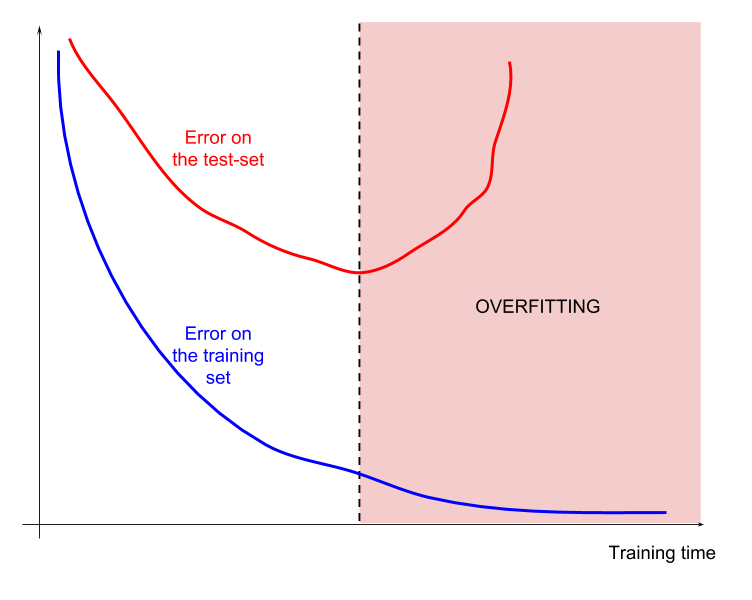
\includegraphics[width=6cm]{mlp_overfitting.png}
\end{center}

Advantages of MLP:
\begin{itemize}
    \item they are universal approximators
    \item they provide posterior probability
    \item many training algorithms are available
\end{itemize}
On the other hand, they are computationally very demanding to train.


\section{Radial basis function neural networks}
A RBF is a function that only depends on the distance between an input vector $\bm x$ and a prototypical vector $\bm x_c$.
$$ \Phi(\norm{\bm x - \bm x_c}) $$
Often, the distance metric used is the euclidean distance.

Common RBF used are the following
\begin{itemize}
    \item gaussian
    \item linear
    \item multiquadratic
    \item cubic
    \item inverse multi-quadratic
    \item thin plate spline
\end{itemize}

RBF NN are used to build up function approximations of the form
$$ F(\bm x) = \sum_{m = 1}^M w_m \Phi(\norm{\bm x - \bm x_{c,m}}) + b $$

Each class will have a specific $F(x)$, each with different weight vector $\bm w$ and bias $b$, but the same RBFs $\Phi(\cdot)$ and centers $x_{c,m}$.

A RBF NN only comprises one input layer, one hidden layer and one output layer.
Since the output layer's activation function is linear, the output $y_i$ for the $i$ class is thus given by
$$ y_i = F_i(\bm x) = \sum_{m = 1}^M w_{m, i} \Phi(\norm{\bm x - \bm x_{c,m}}) + b_i $$

Note that only the connections between the hidden and output layers are weighted.

A popular technique for RBF NN training of the hidden layer's weights is unsupervised clustering using the k-means algorithm.
The algorithm must be configured with a number $k$ of expected classes (in this case, $k = M$, referring to the previous expressions for $y_i$).

The algorithm's steps are the following
\begin{enumerate}
    \item Randomly choose $k$ samples as initial guesses for the barycenters, each related to a different cluster.
    \item Assign each of the remaining samples to the cluster whose barycenter is closest.
    \item For each cluster, update the barycenters as the average of the positions of each sample assigned to the cluster in the previous step.
    \item Go back to step 2, unless the algorithm has converged.
\end{enumerate}

The training of the weights of the output layer is very easy.
Since the output layers have linear activation functions, the problem can be set as a lest square error minimization problem, and solved with the pseudo-inverse technique.

In general, the advantages of RBF NNs are the following
\begin{itemize}
    \item given enough neurons, RBF NNs are universal approximators
    \item RBF NNs provide posterior probability in output
    \item RBF NNs are easily trained
    \item RBF NNs have sample rejection capability: we can detect if a sample is very different (very far) from those used during the training
\end{itemize}

On the other hand
\begin{itemize}
    \item they have potential training instability
    \item separating the training of hidden and output layers limits the accuracy
\end{itemize}


\section{Probabilistic Neural Networks}
PNNs are feed-forward network, based on local basis function.
They allow to perform Bayesian classification with non-parametric pdfs.

Let's consider $C$ classes $\{\omega_1, \dots, \omega_C\}$, each represented by $N_i$ samples $\{\bm x_{i,k}, \dots, \bm x_{i,N_i}\} \in \mathbb R^n$.
PNNs apply the MAP criterion which requires, for each class $\omega_i$, the knowledge of
\begin{itemize}
    \item the class conditional pdf, $\pdf(\bm x | \omega_i)$
    \item the class prior, $\P(\omega_i)$
\end{itemize}

The estimation of the class-conditional pdf is carried out by means of the Parzen window approach.
$$ \widehat{\pdf}(\bm x | \omega_i) = \frac{1}{N_i} \sum_{k = 1}^{N_i} \frac{1}{V(h)} \gamma\left( \frac{\bm x - \bm x_{i, k}}{h} \right) $$
where
\begin{itemize}
    \item $h$ is a parameter to be estimated
    \item $\gamma(\cdot)$ is the so-called kernel function.
    The gaussian kernel is the most widely adopted kernel.
\end{itemize}

The choice of kernel function is very important.
In the case where we use a gaussian kernel with spherical symmetry, then
$$ \widehat{\pdf}(\bm x | \omega_i) = \frac{1}{N_1} \sum_{k = 1}^{N_i} \frac{1}{(2 \pi \sigma^2)^{n/2}} \exp(-\frac{(\bm x - \bm x_{i,k})^2}{2 \sigma^2}) $$

The PNN architecture implements the above formula with artificial neurons.
\begin{center}
    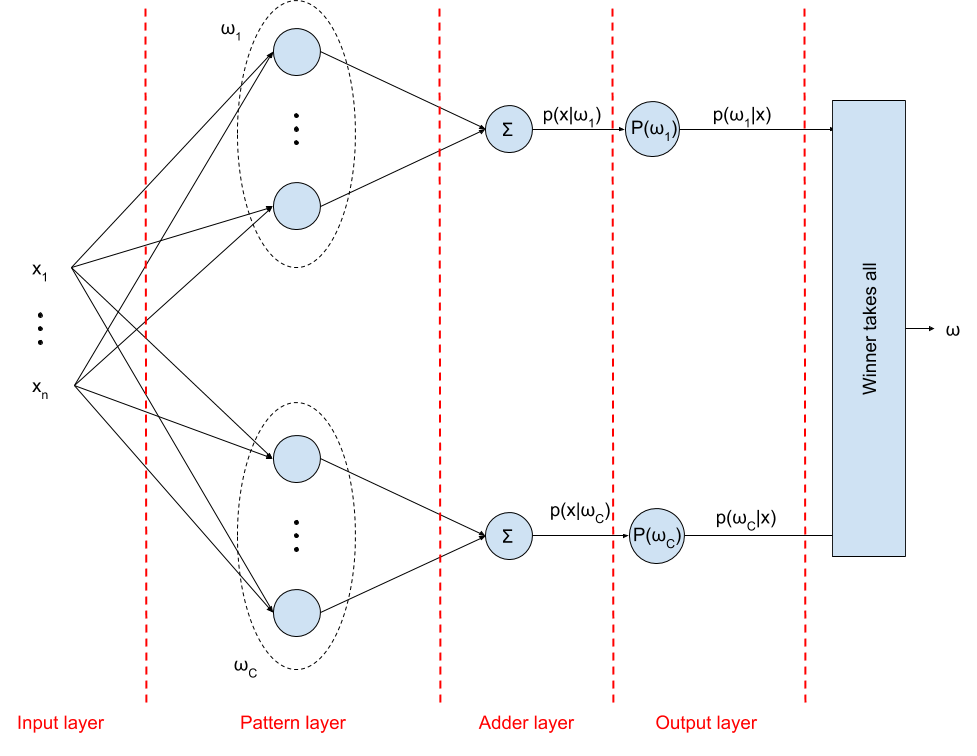
\includegraphics[width=12cm]{probabilistic_neural_network.png}
\end{center}

In the pattern layer, there are $N_i$ neurons for each class $\omega_i$.
The activation function $F_{i,k}(\bm x)$ of the $(i, k)$-th neuron is defined as
\begin{align*}
    F_{i,k}(\bm x)
    &= \exp(-\frac{(\bm x - \bm x_{i,k})^2}{2 \sigma^2}) \\
    &= \exp(-\frac{\norm{\bm x}^2 - 2 \bm x \bm x_{i,k} + \norm{\bm x_{i,k}}^2}{2 \sigma^2})
\end{align*}

Assuming that all the training samples have been normalized to have norm 1, then
\begin{align*}
F_{i,k}(\bm x)
    &= \exp(-\frac{1 - 2 \bm x \bm x_{i,k} + 1}{2 \sigma^2}) \\
    &= \exp(\frac{\bm x \bm x_{i,k} - 1}{ \sigma^2})
\end{align*}

This can be implemented with a perceptron
\begin{itemize}
    \item whose weights are $w_{i,k}$, and
    \item whose activation function is $f_{i, k}(\bm t) = \exp(\frac{\sum_{k=1}^n w_{i, k} t_i - 1}{\sigma})$.
\end{itemize}

Thus, the pattern layer memorizes the training samples!

PNN training means:
\begin{itemize}
    \item determining the smoothing parameter $\sigma$,
    \item computing the weights of the pattern neurons (determined directly from the training samples), and
    \item computing the coefficients of the output layer (i.e. the priors).
\end{itemize}

The advantages of PNNs are that they
\begin{itemize}
    \item only have one free parameter to be tuned,
    \item can be trained fast, and
    \item asymptotically converge to Bayesian error.
\end{itemize}

On the other hand, PNNs
\begin{itemize}
    \item require high memory usage, and
    \item have a slow classification process.
\end{itemize}



\subsection{Adaptive PNNs}
Instead of using $\underline{\underline{\Sigma}} = \sigma \underline{\underline{I}}$, we can use a more general covariance matrix (e.g. diagonal or fully asymmetric).
This increases the number of parameters used, but also the training time



\section{Regression with ANNs}
Assume to have $N$ couples of training samples $\{ (\bm x_i, \bm y_i), i = 1, \dots, N\}$, where
\begin{itemize}
    \item $\bm x_i$ is a feature vector in $\mathbb R^n$, and
    \item $y_i$ is the desired output/target.
\end{itemize}

The objective is finding an approximating function $F(\bm x)$ which optimizes a given accuracy criterion.

This can be implemented in different ways using the architectures explained before:
\begin{itemize}
    \item with an MLP:
    \begin{itemize}
        \item use a single perceptron in the output layer,
        \item use a linear activation function for the output layer,
        \item as many hidden layers as needed.
    \end{itemize}

    \item with a RBF:
    \begin{itemize}
        \item remove the winner takes all at the end,
        \item use a single neuron in the output layer.
    \end{itemize}
\end{itemize}


\subsection{General Regression Neural Networks}
Consider the case where part of the available training samples $(\bm x_i, y_i), i = 1, \dots, N$ have the same value for the input $\bm x_i = \bm x$, but different output values.
How can we chose the best output value $\widehat y$ of our regressor given an input $\bm x$?
We might consider taking the mean of the different $y_i$ values, i.e.
\begin{align*}
    \widehat y
    &= \E{y_i | \bm x_i = \bm x} \\
    &= \int_{-\infty}^{+\infty} y \pdf(y | \bm x) \dd y \\
    &= \int_{-\infty}^{+\infty} y \frac{\pdf(y, \bm x)}{\pdf(\bm x)} \dd y \\
    &= \frac{\int_{-\infty}^{+\infty} y \pdf(y, \bm x) \dd y}{\pdf(\bm x)} \\
    &= \frac{\displaystyle \int_{-\infty}^{+\infty} y \pdf(y, \bm x) \dd y}{\displaystyle \int_{-\infty}^{+\infty} \pdf(y, \bm x) \dd y}
\end{align*}

We need only to find the joint pdf $\pdf(y, \bm x)$.
We can estimate this distribution using the Parzen window method.
First we consider the distribution of $\bm x$.
\begin{align*}
    \widehat \pdf(\bm x)
    &= \frac{1}{N} \sum_{\bm x_i \in X} \frac{1}{V(h)} \gamma\left( \frac{\bm x - \bm x_i}{h} \right) \\
    &= \frac{1}{N} \sum_{\bm x_i \in X} \frac{1}{(2 \pi \sigma^2)^{n/2}} \exp(- \frac{(\bm x - \bm x_i)^T (\bm x - \bm x_i)}{2 \sigma^2})
\end{align*}
where $X$ is the set of the training samples.

Now, let $\bm z = (y, \bm x) \in \mathbb R^{n + 1}$, i.e. a vector concatenating input $y \in \mathbb R$ and output $\bm x \in \mathbb R^n$.
Let $Z$ be the set of the $\bm z_i$ vectors obtained from the training samples $\bm x_i \in X$.
Then
$$
\widehat \pdf(y, \bm x)
= \widehat \pdf(\bm z)
= \frac{1}{N} \frac{1}{(2 \pi \sigma^2)^{\frac{n + 1}{2}}} \sum_i \exp(- \frac{(\bm z - \bm z_i)^T (\bm z - \bm z_i)}{2 \sigma^2})
$$

Now consider the argument of the exponential,
\begin{align*}
    (\bm z - \bm z_i)^T (\bm z - \bm z_i)
    &= (\bm x - \bm x_i, y - y_i)^T (\bm x - \bm x_i, y - y_i) \\
    &= (\bm x - \bm x_i)^T (\bm x - \bm x_i) + (y - y_i)^T (y - y_i) \\
    &= \norm{\bm x - \bm x_i}^2 + (y - y_i)^2
\end{align*}

Therefore
$$
\widehat \pdf(y, \bm x)
= \widehat \pdf(\bm z)
= \frac{1}{N} \frac{1}{(2 \pi \sigma^2)^{\frac{n + 1}{2}}} \sum_i \exp(- \frac{\norm{\bm x - \bm x_i}^2}{2 \sigma^2}) \exp( - \frac{(y - y_i)^2}{2 \sigma^2})
$$

We can now plug this expression of the joint probability in the expression for $\widehat y$ found before.
\begin{align*}
    \widehat y
    &= \frac{\displaystyle \int_{-\infty}^{+\infty} y \pdf(y, \bm x) \dd y}{\displaystyle \int_{-\infty}^{+\infty} \pdf(y, \bm x) \dd y} \\
    &= \frac
        {\displaystyle \int_{-\infty}^{+\infty} y
            \left[
                \frac{1}{N} \frac{1}{(2 \pi \sigma^2)^{\frac{n + 1}{2}}} \sum_i \exp(- \frac{\norm{\bm x - \bm x_i}^2}{2 \sigma^2}) \exp( - \frac{(y - y_i)^2}{2 \sigma^2})
            \right]
        \dd y}
        {\displaystyle \int_{-\infty}^{+\infty}
            \left[
                \frac{1}{N} \frac{1}{(2 \pi \sigma^2)^{\frac{n + 1}{2}}} \sum_i \exp(- \frac{\norm{\bm x - \bm x_i}^2}{2 \sigma^2}) \exp( - \frac{(y - y_i)^2}{2 \sigma^2})
            \right]
        \dd y} \\
    &= \frac
        {\displaystyle
            \cancel{\frac{1}{N} \frac{1}{(2 \pi \sigma^2)^{\frac{n + 1}{2}}}} \sum_i
            \left[
                \exp(- \frac{\norm{\bm x - \bm x_i}^2}{2 \sigma^2})
                \int_{-\infty}^{+\infty} y \exp( - \frac{(y - y_i)^2}{2 \sigma^2}) \dd y
            \right]
        }
        {\displaystyle
            \cancel{\frac{1}{N} \frac{1}{(2 \pi \sigma^2)^{\frac{n + 1}{2}}}} \sum_i
            \left[
                \exp(- \frac{\norm{\bm x - \bm x_i}^2}{2 \sigma^2})
                \int_{-\infty}^{+\infty} \exp( - \frac{(y - y_i)^2}{2 \sigma^2}) \dd y
            \right]
        }
\end{align*}
Note how the numerator and denominator only differ in the argument of the integral, where $y$ is present at the numerator, but not at the denominator.

Now, consider a variable $n$ with gaussian distribution, $n \sim N(\mu, \sigma^2)$.
This means that
$$ \pdf(n) = \frac{1}{\sqrt{2 \pi} \sigma} \exp(- \frac{(n - \mu)^2}{2 \sigma^2}) $$
and
$$ \mu = \E{n} = \int_{-\infty}^{+\infty} n p(n) \dd n = \frac{1}{\sqrt{2 \pi} \sigma} \int_{-\infty}^{+\infty} n \exp(- \frac{(n - \mu)^2}{2 \sigma^2}) \dd n $$

Compare this result with the quantity
$$ \int_{-\infty}^{+\infty} y \exp( - \frac{(y - y_i)^2}{2 \sigma^2}) \dd y $$

Due to the high similarity between the two, we can conclude that
$$ \int_{-\infty}^{+\infty} y \exp( - \frac{(y - y_i)^2}{2 \sigma^2}) \dd y = y_i \sqrt{2 \pi} \sigma $$

Moreover
$$ \int_{-\infty}^{+\infty} \exp( - \frac{(y - y_i)^2}{2 \sigma^2}) \dd y = \left\{ \substack{\text{integral of a gaussian pdf} \\ \text{not normalized}} \right\} = \sqrt{2 \pi} \sigma $$

Thus the expression for $\widehat y$ can be simplified further
\begin{align*}
    \widehat y
    &= \frac
    {\displaystyle
        \sum_i
        \left[
            \exp(- \frac{\norm{\bm x - \bm x_i}^2}{2 \sigma^2})
            \int_{-\infty}^{+\infty} y \exp( - \frac{(y - y_i)^2}{2 \sigma^2}) \dd y
        \right]
    }
    {\displaystyle
        \sum_i
        \left[
            \exp(- \frac{\norm{\bm x - \bm x_i}^2}{2 \sigma^2})
            \int_{-\infty}^{+\infty} \exp( - \frac{(y - y_i)^2}{2 \sigma^2}) \dd y
        \right]
    } \\
    &= \frac
    {\displaystyle
        \sum_i
        \left[
            \exp(- \frac{\norm{\bm x - \bm x_i}^2}{2 \sigma^2})
            y_i \cancel{\sqrt{2 \pi} \sigma}
        \right]
    }
    {\displaystyle
        \sum_i
        \left[
            \exp(- \frac{\norm{\bm x - \bm x_i}^2}{2 \sigma^2})
            \cancel{\sqrt{2 \pi} \sigma}
        \right]
    }
\end{align*}

The numerator is a sum of gaussian kernels, centered in $\bm x_i$, and weighted by $y_i$.
Note that
\begin{itemize}
    \item if $\sigma \to +\infty$, $\widehat y$ is just an average of all the training samples,
    \item if $\sigma \to 0$, the kernels will be very sharp, and the choice of $\widehat y$ will only be affected by the closest samples.
\end{itemize}

The GRNN architecture simply encodes the formula for $\widehat y$.

\begin{center}
    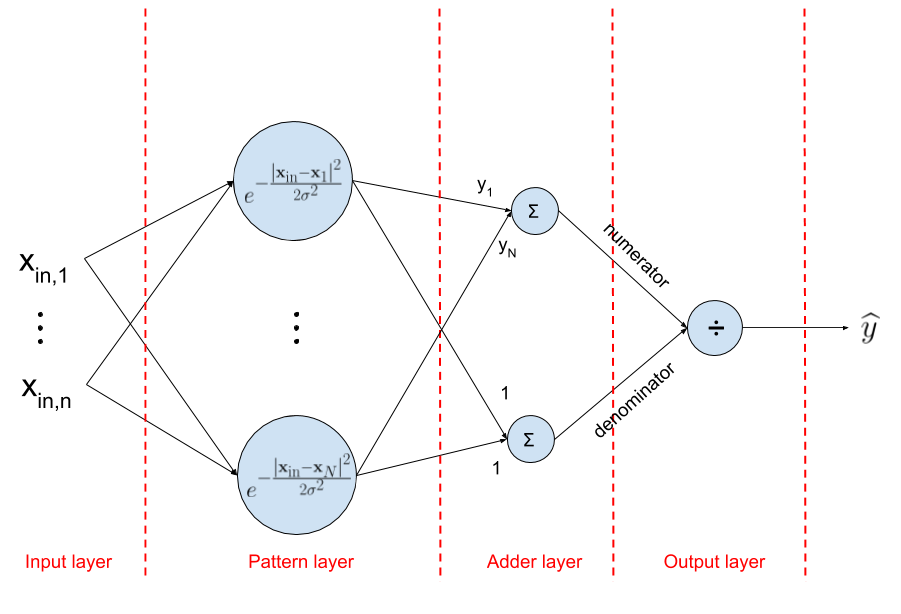
\includegraphics[width=10cm]{general_regression_neural_network.png}
\end{center}

By changing the activation function of the neurons in the pattern layer we can generalize the architecture to work with non-spherically symmetric distributions.

\clearpage
\section{Deep learning}
The classification process can be divided into two steps:
\begin{itemize}
    \item representation, based on hand-chosen features, and
    \item prediction.
\end{itemize}
In DL, the features are extracted by the network itself, they are learned.

DL means using a NN with several hidden layers.

The traditional learning algorithms don't work well with deep architectures.
This is due to the ``vanishing gradient'' effect, where the gradient diminishes in magnitude during back-propagation, yielding poor training of the first layers.

A breakthrough was observed in DL theory around 2006, thanks to
\begin{itemize}
    \item layer-wise training,
    \item unsupervised learning,
    \item hierarchical representation.
\end{itemize}

DL offers a number of advantages
\begin{itemize}
    \item self-extracted features: more complex features than those chosen by hand, with possibility to also include hand-crafted features
    \item unsupervised learning: uses unlabelled data, which is more abundant
    \item multiple levels of representation: similar to what happens in biology
    \item Multi-tasking: the same architecture can work well for very different problems
    \item invariant and disentangling: avoids the curse of dimensionality
\end{itemize}


\subsection{Auto-encoders}
Auto-encoders are NN architectures used for unsupervised learning.
They only consist of an input layer, a hidden layer, and an output layer.
The input and output layer have the same number of nodes.

\begin{center}
    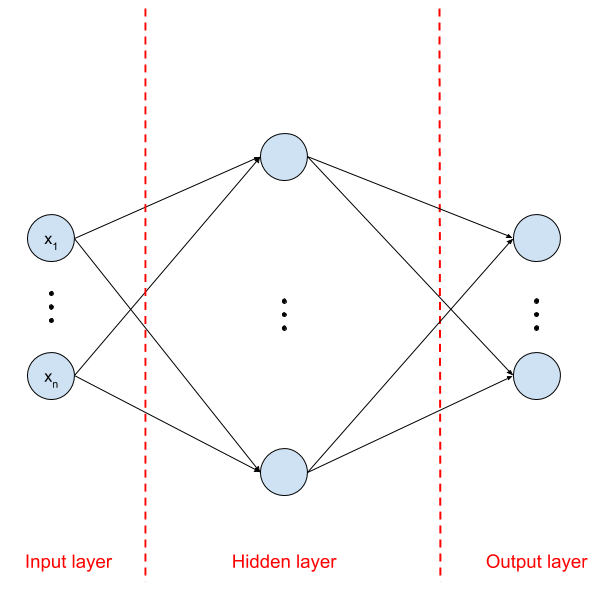
\includegraphics[width=8cm]{autoencoder.png}
\end{center}

The training is performed by using the unlabelled samples both as input and expected output.
In this way, the hidden layer is trained to build a representation that can represent the information content of the samples.

If the number of nodes in the hidden layer is lower than in the other layers, the NN will be forced to extract the most significant features from the samples, thus achieving features extraction.
We can also achieve this with a higher number of neurons, but disabling some of them, i.e. enforcing \textbf{sparsity}.

To enforce sparsity during training we define
\begin{itemize}
    \item $a_j^{(2)}(\bm x)$ is the activation of the $j$-th hidden node given the input $\bm x$
    \item $\widehat \rho_j$ is the average activation of the $j$-th node over all the training samples
    $$ \widehat \rho_j = \frac{1}{N} \sum_{i = 1}^N a_j^{(2)}(\bm x_i) $$
\end{itemize}

We'd like to enforce $\widehat \rho_j$ to be equal to the sparsity parameter $\rho_j$.
To do this, we add a penalty term to the cost function.
This term, takes into account the Kullerback-Leibler divergence between two Bernoulli random variables, with mean $\widehat \rho_j$ and $\rho_j$.

The overall cost function will then take account of
\begin{itemize}
    \item minimizing the MSE of the output, wrt the expected output
    \item minimizing the sum of the KL divergences of each sparsity term
    \item minimize the sum of the squares of all the weights (weight decay term), to prevent over-fitting
\end{itemize}

Consider the case where the input data is an image.
We can visualize what a DL NN has learned to extract?
We can input simple stimuli (like an image with just a single pixel on) and see how this resonates in the NN.

If we use single pixels, we can create a number of ``activation maps'', one per hidden node.
Each pixel of a map is the weight of the input pixel in the same position for the hidden node considered.

The auto-encoder unsupervised training can be used to train each layer of a deeper architecture, one by one (stacked auto-encoders).
After the unsupervised training phase has been performed, a supervised training phase can be performed to fine-tune the network.

Many auto-encoder architectures are available pre-trained


\subsection{Logistic and Softmax regression classifier}
The logistic regression maps all the real values to a value in the $[0,1]$ interval.

The softmax performs a similar operation, but takes $k$ real values in input and outputs $k$ values in the $[0,1]$ interval.
Moreover, the $k$ output variables always sum to 1.

Logistic and softmax regression are not optimal, but they are easy to include in an architecture as they can be trained with back-propagation algorithms.




\subsection{Convolutional Neural Networks}
Fully connected neural networks (like MLP) don't scale well with high number of inputs, for example in the case of large images.
To adapt a neural network architecture to work on visual data we can
\begin{itemize}
    \item resize or sub-sample the image, or
    \item restrict the nodes to number of connections between successive neuron layers.
\end{itemize}

CNN go the second way.
Each node of the input layer is only connected to a number of nodes of the second layer.

For specifically, the CNN work by training filters, that are applied between each layer.
When applying the filter to a layer, we obtain a corresponding feature map.
More filter can be applied at the same layer, to obtain more features maps, also referred to as ``channels''.
Successive layers will then consist in more filters being applied.

Each filter of the input layer consists of a sliding window that is applied on each sample of the input.
Filters of the successive layers also work as sliding window, but are applied on all the channels of the previous layer at once.

Each filter can differ in the size of the window, in the weights of the window, but also in the stride/pace, i.e. the jump in samples between two applications of the same window.
Larger strides allows for reducing the dimensionality of the output, but might result in loss of information.

In general, given an image of size $H \times W$, and a filter whose window has size $a \times b$, the feature map obtained applying the filter will have size $(H - a + 1) \times (W - b + 1)$ (assuming that the stride is 1).

When the number of filters is high, the obtained features are very numerous.
To reduce the number of features we apply the pooling operation.
Pooling is equivalent to a filtering operation with a very high stride, that either performs
\begin{itemize}
    \item maximum extraction: often used in the initial layers of the architecture, as it looses a lot of information,
    \item averaging: often used at the final layers of the neural network.2
\end{itemize}

ReLu activation layers and normalization layers are often used too.
Normalization can be applied
\begin{itemize}
    \item locally (spatial normalization): also referred to as Local Response Normalization,
    \item cross-channel: also considers the other channels.
\end{itemize}

The typical order in which all these operations are performed is the following
\begin{enumerate}
    \item convolutional layer,
    \item ReLu activation layer,
    \item Pooling layer,
    \item Normalization step.
\end{enumerate}

Overall there are many hyper-parameters we can tune in a CNN:
\begin{itemize}
    \item the number of layers,
    \item the number of filters for each layer,
    \item the size of the window of each filter,
    \item the stride of each filter.
\end{itemize}

The CNN is often used to extract a limited a number of features, which is later fed to another NN.

CNN are usually trained with labelled samples.

In 2014, the trained GoogLeNet CNN was published.
It works on 224x224 zero-mean pictures.
Novelties of the GoogLeNet CNN architecture:
\begin{itemize}
    \item To counter the vanishing gradient effect, auxiliary classifiers are inserted at intermediate layers during the training,
    \item Inception module: applies different-sized convolution to achieve multi-scale analysis. Moreover, a number of 1x1 convolutional layers are inserted to achieve feature reduction.
\end{itemize}



\chapter{Support Vector Machine}
\section{Introduction}
The SVM theory was introduced in the 60s, but raised more interest in the 90s.
SVMs are very successful as they overcome the over-fitting problem of MLPs.

SVM are based on the concept of Machine Complexity: by requiring that the system is simple, we obtain higher generalization capabilities and lower over-fitting risk.

Typically, classifiers work in two steps
\begin{itemize}
    \item representation/feature extraction,
    \item decision.
\end{itemize}
In SVM, we suppose that, if the representation step is good enough, the decision step can be simply implemented using linear discriminators.

Linear discriminators use linear decision boundaries, defined by hyper-planes as
$$ \inp{\bm w}{\bm x} + b = 0 $$
where
\begin{itemize}
    \item $\bm x$ is the input feature vector,
    \item $\bm w$ is a vector which is perpendicular to the hyper-plane, and
    \item $b$ is a bias.
\end{itemize}

This is the decision strategy used by the perceptrons.

We introduce the Rosenblat's training algorithm for perceptron.
\begin{enumerate}
    \item Set the initial weight and bias to zero, i.e.
    $$ \bm w_0 = 0, b_0 = 0, k = 0 $$

    \item Compute the radius $R$ equal to the norm of the highest training sample
    $$ R = \max_{\bm x_i}\{\norm{\bm x_i}\} $$

    \item Repeat for increasing values of $k$ until no decision error is obtained on \emph{all} the training samples
    \begin{itemize}
        \item For all $i \in [1, N]$, where $N$ is the number of training samples
        \begin{itemize}[label=\textbullet]
            \item If $y_k (\inp{\bm w_k}{\bm x_i} + b_k) \leq 0$ holds, where $y_i$ is the expected output for the training sample $\bm x_i$
            \begin{itemize}[label=\textbullet]
                \item Update the weights and bias as follows
                $$ \bm w_{k + 1} = \bm w_k + \eta y_i \bm x_i \qquad b_{k + 1} = \eta y_i R^2 $$
                where $\eta$ is the learning rate.
                \item Increase the value of $k$ by 1.
            \end{itemize}
        \end{itemize}
    \end{itemize}
\end{enumerate}

Note that this algorithms only stops if the classes are separable!

\paragraph{Functional and geometrical margins}
Consider a linear discrimination function $f(\bm x) = \inp{\bm w}{\bm x} + b$ such that $f(\bm x) = 0$ is the decision boundary.
Then, given a training sample $\bm x_i$ we define
\begin{itemize}
    \item the functional margin $\gamma_i$ as
    $$ \gamma_i = y_i f(\bm x_i) = y_i (\inp{\bm w}{\bm x_i} + b) $$
    where $y_i$ is $\pm 1$ depending on which class $\bm x_i$ belongs to, and

    \item the geometric margin $\gamma_{g, i}$ as
    $$ \gamma_{g, i} = \frac{y_i f(\bm x_i)}{\norm{\bm w}} = y_i \left( \frac{\inp{\bm w}{\bm x_i}}{\norm {\bm w}} + \frac{b}{\norm{\bm w}} \right) $$
\end{itemize}

A representation of the functional and geometrical margins in a 1-dimensional case ($\bm x_i \equiv x_i \in \mathbb R$) is reported next.
\begin{center}
    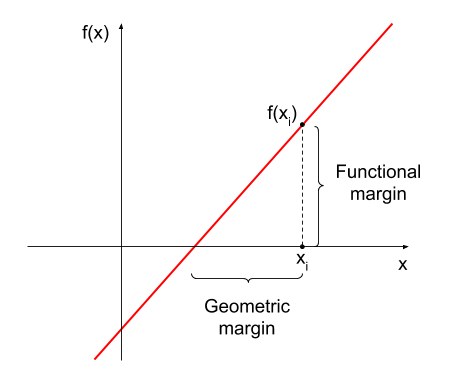
\includegraphics[width=10cm]{functional_and_geometrical_margin.png}
\end{center}

The margin distribution of a given hyperplane $f(\bm x)$ with respect to a set $S$ of training samples is the distribution of the functional margins for the samples in $S$.

The minimum of the margin distribution of a given hyperplane $f(\bm x)$ with respect to a set $S$ is referred to as the margin $\gamma$ of $S$.

The margin $\gamma$ of a training set is the maximum geometric margin over all hyperplanes.

A hyperplane realizing this maximum is called maximal margin hyperplane.

\paragraph{Novikoff's theorem}
Let $S = \{ \bm x_i: i = 1, \dots, N \}$ be a non-trivial training set (meaning it has more than 1 sample).
Let
$$ R = \max_{\bm x \in S} \norm{\bm x} $$
Suppose that there exists a vector $\bm w_\text{opt}$ such that $\norm{\bm w_\text{opt}} = 1$ and
$$ y_i \left( \inp{\bm w_\text{opt}}{\bm x_i} + b_\text{opt} \right) \geq \gamma \qquad \text{for } i = 1, \dots, N $$

Then the number of mistakes made by Rosenblat's perceptron algorithm on the training set $S$ is at most
$$ \left( \frac{2 R}{\gamma} \right)^2 $$

The Novikoff's theorem provides a proof of convergence of Rosenblat's algorithm, because the number of errors is connected to the number of iterations.

Moreover, it proves that
\begin{itemize}
    \item the larger the space ($R \gg 1$), the higher the convergence time, and
    \item the higher the margin of the set $S$ of available training samples, the smaller the convergence time.
\end{itemize}

\paragraph{Slack}
For a given target margin $\gamma > 0$, the margin slack $\xi$ of a training sample $(\bm x_i, y_i)$ with respect to the hyperplane $f(\bm x)$ is
\begin{align*}
\xi
&= \max\{ 0, \gamma - y_i f(\bm x_i) \} \\
&= \max\{ 0, \gamma - y_i (\inp{\bm w}{\bm x_i} + b) \}
\end{align*}

In other words, the slack measures how much a point fails to have a functional margin less than the target margin $\gamma$ from the given hyperplane.

In general, the higher the slack of the training samples, the harder the classification problem (since it means that the samples are little separable).

\paragraph{Dual form}
Note that the term $\bm w_k$ of Rosenblat's algorithm is a scaled sum of $y_i \bm x_i$ values.
Let $\bm w$ be the value of $\bm w_k$ when the algorithm converges, then
$$ \bm w = \sum_{i = 1}^N \alpha_i y_i \bm x_i $$
where $\alpha_i$ is referred to as embedding strength of $\bm x_i$.
It is proportional to the number of times the Rosenblat's algorithm has misclassified the sample $\bm x_i$ during training.

The decision function $h(\bm x)$ can thus be rewritten as
$$
h(\bm x)
= \underbrace{\sgn\{ \inp{\bm w}{\bm x} + b \}}_\text{primal form}
= \underbrace{\sgn \left\{ \sum_{i = 1}^N \alpha_i y_i \inp{\bm x_i}{\bm x} + b \right\}}_\text{dual form}
$$

The whole Rosenblat's algorithm can be rewritten in dual form, to avoid the dependency on $\bm w$
\begin{enumerate}
    \item Initialize the algorithm
    $$ \bm a_0 = 0, b_0 = 0 $$

    \item Compute the radius $R$ equal to the norm of the highest training sample
    $$ R = \max_{\bm x_i}\{\norm{\bm x_i}\} $$

    \item Repeat for increasing values of $k$ until no decision error is obtained on \emph{all} the training samples
    \begin{itemize}
        \item For all $i \in [1, N]$, where $N$ is the number of training samples
        \begin{itemize}[label=\textbullet]
            \item If $y_k \left( \sum_{j = 1}^N \alpha_j y_j \inp{\bm x_j}{\bm x} + b \right) \leq 0$ holds, where $y_i$ is the expected output for the training sample $\bm x_i$
            \begin{itemize}[label=\textbullet]
                \item Update the embedding strength and bias as follows
                $$ \alpha_j = \alpha_j + 1 \qquad b_{k + 1} = \eta y_i R^2 $$
                where $\eta$ is the learning rate.
            \end{itemize}
        \end{itemize}
    \end{itemize}
\end{enumerate}

It can be shown, through Novikoff's theorem, that
$$ \norm{\bm \alpha}_1 \triangleq \sum_{j = 1}^N a_j \leq \left( \frac{2 R}{\gamma} \right)^2 $$

Note that the training samples only enter the algorithm in the dual form through the entries of the so-called \textbf{Gram matrix} $G$, whose entry $G_{i, j}$ in the $i$-th row and $j$-th column is defined as
$$ G = \inp{\bm x_i}{\bm x_j} $$

\paragraph{Ill-definition}
The problem of finding the hyperplane that separates two sets is an ill-defined problem (and thus also an ill-posed problem), as more solution coexists.
We can render the problem well-defined by imposing a criterion to select the best solution among the possible ones, for example
\begin{itemize}
    \item the one that maximises the functional margin
    \item the one that maximises Fisher's discriminant
\end{itemize}

\paragraph{Linear regression}
The linear regression problem is very well-studied.
Find a linear valued function $f(\bm x) = \inp{\bm w}{\bm x} + b$ that best interpolates a given set $S = \{ \bm x_i : i = 1, \dots, N \}$ of training samples labelled with a given set $Y = \{ y_i : i = 1, \dots, N \} \subseteq \mathbb R$.

The best known solution in the case of data corrupted by gaussian noise is the least-squares one.
Let $\widehat{\bm w} = (\bm w^t, b)^t$, and $\widehat X = [\bm x_1, \dots, \bm x_N]^T$ with $\widehat {\bm x}_i = (\bm x_i^T, 1)^T$.
Then the solution is given by
$$ \widehat {\bm w} = \left( \widehat X^T \widehat X \right)^{-1} \widehat X^T \bm y $$

If the matrix is not invertible, or numerical stability problem occur, one can apply the ridge regression or Tichonov regularization.
The solution is then given by
$$ \widehat {\bm w} = \left( \widehat X^T \widehat X + \lambda I \right)^{-1} \widehat X^T \bm y $$

The ridge regression algorithm minimizes the following loss function
$$ L(\bm w, b) = \underbrace{\lambda}_{\substack{\text{balance the} \\ \text{tradeoff}}} \underbrace{ \inp{\bm w}{\bm w}}_{\substack{\text{minimize} \\ \text{the norm}}} + \underbrace{\sum_{i = 1}^N \left( y_i - \inp{\bm w}{\bm x_i} - b \right)^2}_\text{match the samples} $$

Note that the ridge regression also admits a dual representation, where
$$ f(\bm x) = \bm y^T (\lambda I + G)^{-1} \bm z $$
where $z_i = \inp{\bm x}{\bm x_i}$.

\section{Kernel representation}
For complex problems, linear decision boundaries are not sufficient.
Instead, we can transform the $n$-dimensional data in a different space, potentially with higher dimension $n'$, where the linear decision boundaries can be applied effectively.
$$ \bm x \xrightarrow[\substack{\text{representation} \\ \text{process}}]{} \phi(\bm x) \xrightarrow[\substack{\text{decision} \\ \text{process}}]{} y $$

We know that using a too large set of features can create over-fitting problems, because of the curse of dimensionality.
This depends on how the generalization algorithm is controlled.

Thus the actual decision process will be applied to the intermediate representation of the data sample
\begin{gather*}
\begin{dcases}
    y = f(\bm x) = \inp{\bm w}{\phi(\bm x)} + b \\
    \bm w = \sum_{i = 1}^N \alpha_i y_i \phi(\bm x_i)
\end{dcases}
\\
y = f(\bm x) = \sum_{i = 1}^N \alpha_i y_i \inp{\phi(\bm x_i)}{\phi(\bm x)} + b
\end{gather*}

A kernel function allows to do the two processing in a single step.
A kernel is a function $K(\cdot)$ such that for all $\bm x_1, \bm x_2 \in X$,
$$ K(\bm x_1, \bm x_2) = \inp{\phi(\bm x_1)}{\phi(\bm x_2)} $$
where $\phi(\cdot)$ is a mapping from $X$ to another feature space $F$.

Thus
$$ y = f(\bm x) = \sum_{i = 1}^N \alpha_i y_i K(\bm x_i, \bm x) + b $$

This is very similar to what we've seen in RBF.

\paragraph{How to build a kernel?}
In the case where the representation step is a simple linear transformation and $\phi(\bm x) = A \bm x$, then
$$ K(\bm x_1, \bm x_2) = \inp{A \bm x_1}{A \bm x_2} = \bm x_1^T A^T A \bm x_2 = \bm x_1^T B \bm x_2 $$
In this case, the dimensionality of the sample space and the representation space are the same, $n = n'$.

However, this might not be the case for non-linear transformations like
$$ K(\bm x_1, \bm x_2) = \inp{\bm x_1}{\bm x_2}^2 $$
In that case
\begin{align*}
    K(\bm x_1, \bm x_2)
    &= \inp{\bm x_1}{\bm x_2}^2 \\
    &= \inp{\bm x_1}{\bm x_2} \inp{\bm x_1}{\bm x_2} \\
    &= \left( \sum_{i = 1}^n x_{1, i} x_{2, i} \right) \left( \sum_{i = 1}^n x_{1, i} x_{2, i} \right) \\
    &= \begin{vmatrix}
        x_{1, 1}^2 x_{2, 1}^2 & x_{1, 1} x_{2, 1} x_{1, 2} x_{2, 2} & \dots & x_{1, 1} x_{2, 1} x_{1, n} x_{2, n} \\
        x_{1, 2} x_{2, 2} x_{1, 1} x_{2, 1} & x_{1, 2}^2 x_{2, 2}^2 &  & \vdots \\
        \vdots &  & \ddots & \\
        x_{1, n} x_{2, n} x_{1, 1} x_{2, 1} & \dots & & x_{1, n}^2 x_{2, n}^2
    \end{vmatrix}_1
\end{align*}
However, the matrix is symmetric, thus the number of unique elements is
$$ n' = \frac{n^2 - n}{2} - n = \binom{n + 1}{2} $$

What if we add a constant?
\begin{align*}
    K(\bm x_1, \bm x_2)
    &= (\inp{\bm x_1}{\bm x_2} + c)^2 \\
    &= \inp{\bm x_1}{\bm x_2}^2 + 2 c \inp{\bm x_1}{\bm x_2} + c^2
\end{align*}

The first term gives the same number of binomials as the previous result, the second yields $n$ monomials and the third term results in 1 one more term, totaling
$$ n' = \binom{n + 1}{2} + n + 1 = \binom{n + 2}{2} $$

More generally
$$ K(\bm x_1, \bm x_2) = \inp{\bm x_1}{\bm x_2}^d \implies n' = \binom{n + d - 1}{d} $$
and
$$ K(\bm x_1, \bm x_2) = (\inp{\bm x_1}{\bm x_2} + c)^d \implies n' = \binom{n + d}{d} $$

\paragraph{Mercer's condition}
There exists a mapping $\phi(\cdot)$ and an expansion
$$ K(\bm x_1, \bm x_2) = \sum_{i = 1}^{n'} \phi(x_1) \phi(x_2) $$
if and only if, for any $g(\bm x)$ such that
$$ \int g(\bm x)^2 \dd \bm x \text{ is finite} $$
then
$$ \int_{-\infty}^{+\infty} K(\bm x_1, \bm x_2) g(\bm x_1) g(\bm x_2) \dd \bm x_1 \dd \bm x_2 \geq 0 $$

In other words, $K(\cdot)$ is a Mercer kernel function if it is continuous, symmetric and non-negative definite.

The kernel matrix or Gram matrix is defined for a finite subset $\{\bm x_1, \dots \bm x_m\}$ of $X$ as
$$ \bm K_{i, j} = K(\bm x_i, \bm x_j) $$

The kernel matrix is a symmetric positive semi-definite.
Any symmetric positive semi-definite matrix can be viewed as a kernel matrix, that is as an inner product matrix in some space.

The kernel matrix is the central structure in kernel machine, since it conveys all necessary information (from the considered problem) for the learning algorithm.

Consider the value of the kernel matrix between two points $\bm x_1, \bm x_2$.
The euclidean distance between the representation of the two points would be
$$ \norm{\phi(\bm x_1) - \phi(\bm x_2)}^2
= \norm{\phi(\bm x_1)}^2 - 2 \inp{\phi(\bm x_1)}{\phi(\bm x_2)} + \norm{\phi(\bm x_2)}^2 $$

Assuming that $\norm{\phi(\bm x_i)}^2 = 1 \; \forall i$, then
\begin{align*}
    \norm{\phi(\bm x_1) - \phi(\bm x_2)}^2
    &= \norm{\phi(\bm x_1)}^2 - 2 \inp{\phi(\bm x_1)}{\phi(\bm x_2)} + \norm{\phi(\bm x_2)}^2 \\
    &= 2 - 2 \inp{\phi(\bm x_1)}{\phi(\bm x_2)} \\
    &= 2 (1 - K(\bm x_1, \bm x_2))
\end{align*}

Then
$$ K(\bm x_1, \bm x_2) = 1 - \frac{\norm{\phi(\bm x_1) - \phi(\bm x_2)}^2}{2} $$

Thus, the $\bm K$ matrix computes the distance between the samples in the transformed space.

\paragraph{Bad kernel}
Consider the following kernel
$$ \bm K = \begin{bmatrix}
    1 & 0 & 0 \\
    0 & 1 & 0 \\
    0 & 0 & 1
\end{bmatrix} $$

Remembering that
$$ \norm{\phi(\bm x_i) - \phi(\bm x_j)}^2 = 2 (1 - K(\bm x_i, \bm x_j)) $$

We can conclude that
$$ \left[ \norm{\phi(\bm x_i) - \phi(\bm x_j)}^2 \right] = 2 (1 - \bm K) = \begin{bmatrix}
    0 & 2 & 2 \\
    2 & 0 & 2 \\
    2 & 2 & 0
\end{bmatrix} $$

This means that all the samples $\bm x_i, i = 1, 2, 3$ are equidistant from each other in the transformed dimension.
Geometrically, this means that they are located on three different axis (or 3 orthogonal directions), at the same distance from their barycentre.

This means that all the points form a different cluster, with no hint on characterizing structures.

An even worse kernel is the following
$$ \bm K = \begin{bmatrix}
    1 & 1 & 1 \\
    1 & 1 & 1 \\
    1 & 1 & 1
\end{bmatrix} $$

Following the same steps as before,
$$ \left[ \norm{\phi(\bm x_i) - \phi(\bm x_j)}^2 \right] = 2 (1 - \bm K) = \begin{bmatrix}
    0 & 0 & 0 \\
    0 & 0 & 0 \\
    0 & 0 & 0
\end{bmatrix} $$

This means that all the different points coincide in the transformed dimension, and are thus perfectly overlapping.

\section{Closure properties of kernels}
Starting from a kernel we can build other kernels using a number of manipulations, in particular
\begin{enumerate}
    \item summing two kernels
    \item multiplying a kernel by a constant
    \item multiplying two kernels
    \item $K(\bm x_1, \bm x_2) = f(\bm x_1) f(\bm x_2)$, where $f(\cdot)$ is a real valued function
    \item applying a kernel on a different representation $\phi_2(\cdot)$
    \item $K(\bm x_1, \bm x_2) = \bm x_1^T B \bm x_2$, where $B$ is symmetric positive semi-definite
    \item $K(\bm x_1, \bm x_2) = p(K_1(\bm x_1, \bm x_2))$, where $p(\cdot)$ is a polynomial with positive coefficients
    \item $K(\bm x_1, \bm x_2) = \exp(K_1(\bm x_1, \bm x_2))$
\end{enumerate}

We can show that the Gaussian Kernel is a valid kernel.
In fact
\begin{align*}
    \exp(-\frac{\norm{\bm x_1 - \bm x_2}^2}{\sigma^2})
    &= \exp(-\frac{\norm{\bm x_1}^2 + \norm{\bm x_2}^2 - 2 \inp{\bm x_1}{\bm x_2}}{\sigma^2}) \\
    &=
    \underbrace{
        \underbrace{\exp(-\frac{\norm{\bm x_1}^2}{\sigma^2})}_{f(\bm x_1)}
        \underbrace{\exp(\frac{\norm{\bm x_2}^2}{\sigma^2})}_{f(\bm x_2)}
    }_{K_1(\bm x_1, \bm x_2) \text{ valid for rule \#4}}
    \underbrace{\exp(-\frac{2 \inp{\bm x_1}{\bm x_2}}{\sigma^2})}_{K_2(\bm x_1, \bm x_2) \text{ valid for rule \#8}} \\
    &= \underbrace{K_1(\bm x_1, \bm x_2) K_2(\bm x_1, \bm x_2)}_\text{valid for rule \#3}
\end{align*}

\section{Generalization theory}
How can we guarantee good generalization properties?
Kernels allow higher expressive power, but increase over-fitting risk.
Many theories allow to estimate the generalization error.
We're going to cover the Vapnik–Chervonenkis theory.

The \textbf{capacity} of a machine is the ability to classify/discriminate two classes without any error.

Consider the case of two botanists, that have to recognize whether a photo represents a plant or not:
\begin{itemize}
    \item the first botanist, has a photographic memory, and can remember all the plants he has seen in his life. He is very accurate on the training set. However, when handed a photo of a plant, he might not recognize it because it does not perfectly represent a plant (e.g. because the picture is taken from a different angle). He incurs into the over-fitting problem.
    \item the second botanist is lazier, and only discriminates based on the amount of green parts in the photo. He will be able to classify a higher number of pictures, but with a low accuracy, as he is under-fitting.
\end{itemize}

This example is to highlight the need to balance
\begin{itemize}
    \item the accuracy level obtained on the training set, and
    \item the capacity of the machine.
\end{itemize}

\section{Generalization error}
Consider a simple regression problem, where we're trying to find the best guess for an unknown function $f_\text{real}(\bm x)$ that maps $\bm x_i$ samples into the corresponding $y_i$ value.

We define the hypothesis space as the set of all the possible solutions given by our machine, e.g. the set of all linear functions.
This space can be defined by a-priori information about the problem or by limits in our machine.

However, the true function might not be present in the hypothesis space.
This introduces an \textbf{approximation error}., which can not be overcome.
The approximation error will be equal to the minimum distance between the true function and any element of the hypothesis space.

Moreover, when applying the regression algorithm, we might introduce an error in the estimation of the parameters (e.g. due to a limit in the number of iterations allowed).
This is referred to \textbf{estimation error}.

The \textbf{generalization error} is the sum of the approximation error and estimation error.

The approximation is easier to solve, as it is sufficient to expand the hypothesis space.

We will now try to compute the expectation of the generalization error.
Assume that there exists some unknown joint probability distribution $\P(\bm x, y)$ from which training samples are drawn.
Moreover, assume that the samples are independent and identically distributed.
Assume that the machine is defined by a set of possible mappings $f(\bm x, \alpha): \bm x \mapsto y$, where the functions are labelled by the adjustable parameter $\alpha$.
Also, assume that the machine is deterministic, i.e. for a given choice of $\bm x$ and $\alpha$, it will always give the same output. A particular choice of parameters generates a trained machine.

We can compute the risk given $\alpha$, as an expectation
$$ R(\alpha) = \E{R(\alpha | \bm x, y)} = \int_{\bm x} \int_y R(\alpha | \bm x, y) \pdf(\bm x, y) \dd y \dd \bm x $$
where $R(\alpha | \bm x, y)$ is a user-defined cost function.
For instance, the the square error could be used
$$ R(\alpha | \bm x, y) = (f(\bm x, \alpha) - y)^2 $$

However, the expression found for $R(\alpha)$ requires the knowledge of the joint distribution $\pdf(\bm x, y)$, which is not available to us.
Instead we can use the training sample to approximate the risk, computing the so-called \textbf{empirical risk} $R_\text{emp}(\alpha)$
$$ R(\alpha) \approx R_\text{emp}(\alpha) = \frac{1}{N} \sum_{i = 1}^N R(\alpha| \bm x_i, y_i) $$

Vapnik and Chervonenkis proposed improving the knowledge of the generalization error finding an upper bound of the risk, which is the following
$$ R(\alpha) \leq R_\text{emp}(\alpha) + \underbrace{\sqrt{\frac{h(\log(2 N / h) + ) - \log(\eta/4)}{N}}}_\text{VC confidence} $$
where
\begin{itemize}
    \item $\eta$ is the confidence of the bound, meaning that the bound holds with probability $1 - \eta$, and
    \item $h$ is the VC dimension, which will be defined later.
\end{itemize}
Note that the upper bound does not depend any more on the joint probability distribution $\pdf(\bm x, y)$.

\section{VC dimension}
Consider a set of $N$ samples labelled with either one of two classes, and a class of machines $\{f(\alpha)\}$.
If for all the possible $2^N$ labelling of the $N$ samples, there exists a machine $f(\alpha)$ of the class consider that correctly classifies all the samples, then we say that this set of point is \textbf{shattered} by the class of functions $\{f(\alpha)\}$.

The VC dimension $h$ of a given class of machines $\{f(\alpha)\}$ is defined as the maximum number of training samples that can be shattered by the considered class.

If the VC dimension $h$ of a class of machine is equal to the number of available samples $N$, the VC dimension is said to be ``infinite''.
In this case, the risk bound is not valid.

Note that the VC dimension only depends on the number of samples and not on their position.

Also note that, if the VC dimension of a machine class $h$, the class might only shatter one specific set of size $h$, and not all possible sets.

\paragraph{Theorem}
Consider some set of $m$ points in $\mathbb R$.
Choose any one of the points as origin.
Then the $m$ points can be shattered by oriented hyperplanes if and only if the position vectors of the remaining points are linearly independent.

A consequence of the above theorem is that the VC dimension of a set of $n$ hyperplanes in $\mathbb R^n$ is
$$ h = n + 1 $$

Thus, when choosing which class of machines to use for a specific classification problem
\begin{itemize}
    \item if the empirical risk of all the candidate classes is equal, we choose the one with minimal VC dimension, and
    \item if the empirical risk is different, then we choose the one with minimal risk bound.
\end{itemize}

\subsection{Structural Risk Minimization}
SRM is an inductive principle for choosing the best machine class.
It is based on the fact that,
\begin{itemize}
    \item the VC confidence $h$ is the same for all the machines of a particular class (i.e. independent of $\alpha$), whereas
    \item the empirical risk $R_\text{emp}(\alpha)$ depends on the particular function chosen by the training procedure (i.e. dependent of $\alpha$).
\end{itemize}
The idea behind SRM is that of
\begin{enumerate}
    \item given a set of candidate machines, compute the VC dimension for each of them
    \item divide the set of machines into subsets of machines with the same VC dimension
    \item for each of these subsets, select the machine minimizing the empirical risk
    \item among these selected machines, choose the one minimizing the risk bound
\end{enumerate}

\begin{center}
    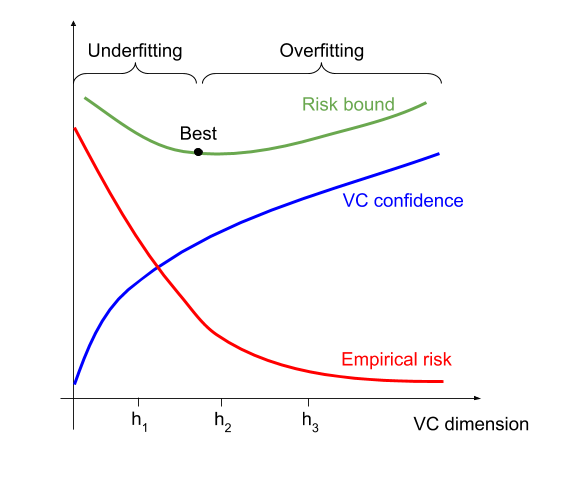
\includegraphics[width=10cm]{structural_risk_minimzation.png}
\end{center}

There are some problems with this approach
\begin{itemize}
    \item it is not straightforward to compute the VC dimension of a machine
    \item the VC dimension could be infinite, or the compute risk bound might be higher then 1
    \item the VC confidence does not help in making the perceptron training problem well-defined (more than one solution to the problem)
\end{itemize}


\section{Margin-based bounds}
Margin based bounds are used to tighten the upper bound on the expected risk.

Suppose that $f(\bm x)$ is a real-valued function that will be thresholded at 0 to give $y$,
$$ y = \sgn\{f(\bm x)\} $$
The functional margin $\gamma_i$ of $f(\cdot)$ on the $i$-th training sample $(\bm x_i, y_i)$ is
$$ \gamma_i = y_i f(\bm x_i) $$
The (functional) margin distribution $M_S(f)$ for $f(\cdot)$ over the training set $S = \{ (\bm x_i, y_i) : i = 1, \dots, N \}$ is then
$$ M_S(f) = \{ \gamma_i : i = 1, \dots, N \} $$
The margin with respect to the whole training set $S$ is defined as the minimum over the the margin distribution $M_S(f)$
$$ \gamma = \min\{ M_S(f) \} $$

\subsection{Margin-based bound}
Consider the space of real valued functions $F$, that will be thresholded at 0 to give $Y$.
This space has some VC dimension $h$.

But now, suppose that we consider thickening each function $f(\cdot) \in F$ by requiring that it correctly classifies every point with a margin of at least $\gamma$.
The VC dimension of these ``fat'' separator is called \textbf{fat-shattering dimension}, $fat_F(\gamma)$, and will be less than the previous $h$ value.

\paragraph{Theorem}
Suppose that $X$ is the ball of radius $R$ in an inner product space $\Psi$.
Consider the class of functions
$$ F = \{ f: \bm x \mapsto \inp{\bm w}{\bm x} : \norm{\bm w} \leq 1, \bm x \in X\} $$
Then
$$ fat_F(\gamma) \leq \left( \frac{R}{\gamma} \right)^2 $$

The above theorem proves that minimizing $\gamma$ reduces the machine complexity and thus increases the generalization capabilities.

\paragraph{Theorem}
Consider thresholding real-valued linear functions $F$ with unit weight vectors on an inner product space $X$ and fix $y \in \mathbb R^+$.
For any probability distribution $P$ on $X \times \{-1, 1\}$, with support in a ball of radius $R$ around the origin, with probability $1 - \eta$ over $N$ random examples $S$, any hypothesis $f \in F$ that has margin greater or equal than $\gamma$ on $S$, has error of no more than
$$ \frac{2}{N} \left[ \frac{64 R^2}{\gamma^2} \log(\frac{e N \gamma}{4 R}) \log(\frac{128 N R^2}{\gamma^2}) - \log(\frac{\eta}{4}) \right] $$
provided that $N > 2/\eps$ and $N > 64 R^2 / \gamma$.

Note that
\begin{itemize}
    \item this bound does not depend on the dimensionality of the transform space, $n'$
    \item if $\gamma = 0$ (classes are not separable), the bound diverges
    \item again, maximizing $\gamma$ reduces the bound
\end{itemize}

\subsubsection{Soft margin-based bound}
Can we find something like the margin-based bound that can work with non-separable classes?

We define the margin slack variables $\xi_i, i = 1, \dots, N$ as
$$ \xi_i = \xi((\bm x_i, y_i), f, \gamma) = \max(0, \gamma - y_i f(\bm x_i)) $$

The margin slack vector $\bm \xi$ is thus
$$ \bm \xi = \{ \xi_i : i = 1, \dots, N \} $$

\paragraph{Theorem}
Consider thresholding real-valued linear functions $F$ with unit weight vectors on an inner product space $X$ and fix $y \in \mathbb R^+$.
There is a constant $c$, such that for any probability distribution $P$ on $X \times {-1, 1}$, with support in a ball of radius $R$ around the origin, with probability $1 - \eta$ over $N$ random examples $S$, any hypothesis $f \in F$  has error of no more than
$$ \frac{c}{N} \left[ \frac{R^2 + \norm{\bm \xi}_{1, 2}^2 \tau}{\gamma^2} \log^2(N) - \log(\eta) \right] $$
where $\norm{\bm \xi}_{1, 2}$ is either the $l$-1 or $l$-2 norm of the margin slack vector, and
$$ \tau = \begin{cases}
    \log(1 / \gamma) & \text{if the $l$-1 norm is used} \\
    1 & \text{otherwise}
\end{cases} $$

Here, a constant $c$ appears in the theorem without a way to computing it.
However, this is not a problem, since we use the results from this theorem to compare different machines, assuming that the $c$ constant is the same for all the machines.

Here, to tighten the bound we need to maximize $\norm{\bm \xi}^2 / \gamma$.

\subsubsection{Generalization for regression}
In this section we'll try to translate the margin concepts from classification to regression.

In regression the mismatch between the expected and actual output is continuous, and not discrete like in classification.
The difference is referred to as \textbf{residual}.

Moreover, in regression we are usually interested in achieving a finite accuracy.
This is formalized by admitting errors below a certain threshold $\theta$.
For regression, the slack is then defined in a slightly different way.
Given the $i$-th training samples $(\bm x_i, y_i)$, the regression function $f(\cdot)$, the margin $\gamma$ and the required accuracy $\theta$, then the slack is
$$ \xi_i = \xi((\bm x_i, y_i), f, \gamma, \theta) = \max(0, \abs{y_i - f(\bm x)} - (\theta - \gamma)) $$

\begin{center}
    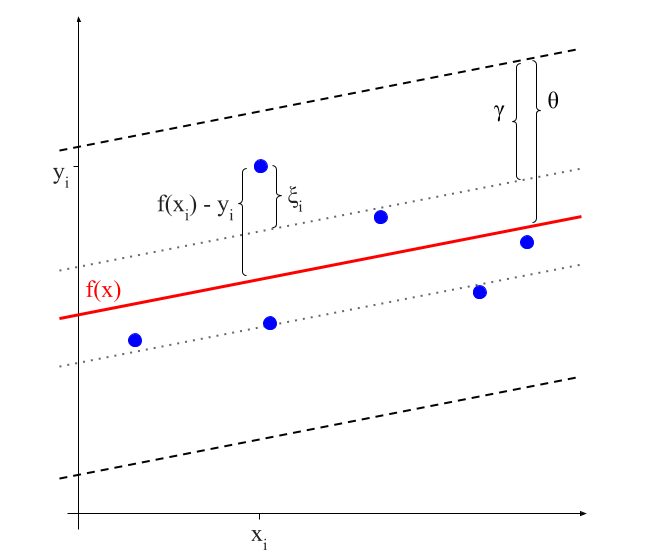
\includegraphics[width=10cm]{regression_slack.png}
\end{center}

\paragraph{Theorem} Consider performing regression with linear functions $F$ on an inner product space $X$ and fix $\gamma < \theta, \gamma \in \mathbb R^+$.
There is a constant $c$, such that for any probability distribution $P$ on $X \times \mathbb R$, with support in a ball of radius $R$ around the origin, with probability $1 - \eta$ over $N$ random examples $S$, the probability that a hypothesis $\bm w \in F$ has output more than $\theta$ away from its true value is bounded by
$$ \frac{c}{N} \left[ \frac{R^2 \norm{\bm w}^2_2 + \norm{\bm \xi}_{1, 2}^2 \tau}{\gamma^2} \log^2(N) - \log(\eta) \right] $$
where $\norm{\bm \xi}_{1, 2}$ is either the $l$-1 or $l$-2 norm of the margin slack vector, and
$$ \tau = \begin{cases}
    \log(1 / \gamma) & \text{if the $l$-1 norm is used} \\
    1 & \text{otherwise}
\end{cases} $$

In the case where $\gamma = \theta$, then we're not tolerating any error, and minimizing the soft margin bound is equivalent to minimizing $\norm{\bm w}^2$ and $\abs{\sum_{i = 1}^N (y_i + f(\bm x_i))^2}$

We can also see soft-margin as a way to differentiate the tolerance between training (no error larger than $\theta - \gamma$, strict) and during the actual regression (no error larger than $\theta$, lax).


\section{Support Vector Machine}
SVM are machines for efficiently training linear machines
\begin{itemize}
    \item in the kernel induced feature space,
    \item respecting the insights produced by generalization theory,
    \item exploiting optimization theories.
\end{itemize}

The two key concepts of SVM are
\begin{itemize}
    \item sparseness, and
    \item convexity (allowing a unique optimal solution).
\end{itemize}

In the few last sections we have introduced a number of bounds.
All machines minimizing any of these bounds are referred to as SVMs.

\subsection{Maximal Margin Classifier}
The MMC constitutes the simplest SVM.
It requires that the classes are linearly separable.
The idea at its heart is to minimize the margin-based bound.

The margin-based bound is expressed in terms of the geometric margin $\gamma$.
To decrease the bound, we should maximize the margin.
But there are infinitely as many planes yielding the same geometric margin.
How can we make the problem well-defined?

The idea is to constraint the functional margin to be 1 for the samples $\bm x^+$ and $\bm x^-$ that are closest to the margin for the two classes respectively.

\begin{gather*}
    \begin{cases}
        y^+ f(\bm x^+) = 1 \\
        y^- f(\bm x^-) = 1
    \end{cases}
\end{gather*}

The geometric margin $\gamma$ is given by
$$ \gamma = \frac{y^+ f(\bm x^+)}{\norm{\bm w}} \text{ and } \gamma = \frac{y^- f(\bm x^-)}{\norm{\bm w}} $$

Then
$$ \gamma = \frac{\gamma + \gamma}{2} = \frac{\displaystyle \frac{y^+ f(\bm x^+)}{\norm{\bm w}} + \frac{y^- f(\bm x^-)}{\norm{\bm w}}}{2} = \frac{f(\bm x^+) - f(\bm x^-)}{2 \norm{\bm w}} $$

For the samples that are not closest to the margin we want
$$ y_i f(\bm x_i) \geq 1 \quad \text{for } i = 1, \dots, N $$

Resuming, the optimal solution is the one
\begin{itemize}
    \item with the lowest slope, $\norm{\bm w}$,
    \item and that satisfies $y_i f(\bm x_i) \geq 1 \quad \text{for } i = 1, \dots, N $
\end{itemize}

This yields us to the \textbf{Primal Optimization Problem} for the MMC.
\begin{align*}
    &\text{Minimize   } \quad \psi(\bm w) = \frac{1}{2} \norm{\bm w}^2 \\
    &\text{Subject to } \quad y_i f(\bm x_i) \geq 1 \quad \text{for } i = 1, \dots, N
\end{align*}

Note that this problem has no solution if the classes are not linearly separable.

This is a constrained optimization problem, and could be solved with the Lagrangian multipliers if only equality constraints are present.

We will now introduce the Karush-Kuhn-Tucker conditions, that allow to generalize the Lagrangian multipliers method to problems with inequality constraints.

\paragraph{Karush-Kuhn-Tucker conditions}
Given an optimization problem with convex domain $\Omega \subseteq \mathbb R^n$ of the type
\begin{align*}
    &\text{Minimize   } \quad \psi(\bm w), \bm w \in \mathbb R^n \\
    &\text{Subject to } g_i(\bm w) \leq 0, \text{for } i = 1, \dots, k, \\
    &\text{           } h_j(\bm w) = 0, \text{for } j = 1, \dots, m
\end{align*}
with $f \in C^1$ convex and $g_i, h_j$ affine, necessary and sufficient conditions for a normal point $\bm w^+$ to be an optimum are the existence of $\bm \alpha^*$ and $\bm \beta^+$ such that
$$
\begin{dcases}
    \pdv{L(\bm w^+, \bm \alpha^*, \bm \beta^+)}{\bm w} = 0 \\
    \pdv{L(\bm w^+, \bm \alpha^*, \bm \beta^+)}{\bm \beta} = 0 \\
    \alpha_i^* g_i(\bm w^*) = 0 \quad \text{for } i = 1, \dots, k \\
    g_i(\bm w^*) \leq 0 \quad \text{for } i = 1, \dots, k \\
    \alpha_i(\bm w^*) \geq 0 \quad \text{for } i = 1, \dots, k \\
\end{dcases}
$$
where $L(\cdot)$ is the generalized Lagrangian function.
The KT theorem will be also useful for other SVMs shown later.

We will now apply the KKT conditions to our problem.
We'll rewrite the constraints to make the constraint function $g_i(\bm w)$ more explicit.
\begin{align*}
    &\text{Minimize   } \quad \psi(\bm w) = \frac{1}{2} \norm{\bm w}^2 \\
    &\text{Subject to } \quad g_i(\bm w) = 1 - y_i f(\bm x_i) = 1 - y_i (\inp{\bm w}{\bm x_i} + b) \leq 0 \quad \text{for } i = 1, \dots, N
\end{align*}


The Lagrangian is
$$ L(\bm w, b, \bm \alpha) = \frac{1}{2} \norm{\bm w}^2 + \sum_{i = 1}^N \alpha_i [1 - y_i (\inp{\bm w}{\bm x_i} + b)] $$

Differentiating with respect to $\bm w$ and $b$, and imposing stationarity (i.e. partial derivatives equal to zero)
$$ \begin{dcases}
    \pdv{L(\bm w, b, \bm \alpha)}{\bm w} = \bm w - \sum_{i = 1}^N y_i \alpha_i \bm x_i = 0 \\
    \pdv{L(\bm w, b, \bm \alpha)}{b} = \sum_{i = 1}^N y_i \alpha_i = 0
\end{dcases} \implies
\begin{dcases}
    \bm w = \sum_{i = 1}^N y_i \alpha_i \bm x_i \\
    \sum_{i = 1}^N y_i \alpha_i = 0
\end{dcases}
$$

Substituting this into the primal problem yields the dual problem's Lagrangian
\begin{align*}
    L(\bm w, b, \bm \alpha)
    &= \frac{1}{2} \norm{\bm w}^2 + \sum_{i = 1}^N \alpha_i [1 - y_i (\inp{\bm w}{\bm x_i} + b)] \\
    &= \frac{1}{2} \inp{\bm w}{\bm w} + \sum_{i = 1}^N \alpha_i - \sum_{i = 1}^N \alpha_i y_i \inp{\bm w}{\bm x_i} - b \underbrace{\sum_{i = 1}^N \alpha_i y_i}_0 \\
    &= \frac{1}{2} \sum_{i = 1}^N \sum_{j = 1}^N \alpha_i \alpha_j y_i y_j \inp{\bm x_i}{\bm x_j} + \sum_{i = 1}^N \alpha_i - \sum_{i = 1}^N \sum_{j = 1}^N \alpha_i \alpha_j y_i y_j \inp{\bm x_i}{\bm x_j} \\
    &= \sum_{i = 1}^N \alpha_i - \frac{1}{2} \sum_{i = 1}^N \sum_{j = 1}^N \alpha_i \alpha_j y_i y_j \inp{\bm x_i}{\bm x_j}
\end{align*}

The dual optimization problem is then
\begin{align*}
    &\text{Maximize   } \quad \psi(\bm a) = \sum_{i = 1}^N \alpha_i - \frac{1}{2} \sum_{i = 1}^N \sum_{j = 1}^N \alpha_i \alpha_j y_i y_j \inp{\bm x_i}{\bm x_j} \\
    &\text{Subject to } \quad \begin{dcases}
    \sum_{i = 1}^N y_i \alpha_i = 0 \\
    a_i \geq 0
\end{dcases} \quad \text{for } i = 1, \dots, N
\end{align*}

As you can see, the cost function of the dual problem does not depend on $\bm w$ and $b$, but only on $\bm \alpha$.
We thus have obtained a quadratic problem with linear constraints, which has a unique solution that can be easily found.

Once the optimal $\bm \alpha^*$ is found, the corresponding optimal weight vector $\bm w^+$ and margin $\gamma$ are found as
$$ \bm w^* = \sum_{i = 1}^N y_i \alpha_i^* \bm x_i \quad \text{and} \quad \gamma = \frac{1}{\norm{\bm w^*}}$$

The value of $b$ can instead be found making use of the primal constraints.
\begin{gather*}
    \begin{dcases}
        y^+ f(\bm x^+) = 1 \\
        y^- f(\bm x^-) = 1
    \end{dcases} \\
    \begin{dcases}
        f(\bm x^+) = +1 \\
        f(\bm x^-) = -1
    \end{dcases} \\
    f(\bm x^+) + f(\bm x^-) = 0 \\
    \inp{\bm w^*}{\bm x^+} + b^* + \inp{\bm w^*}{\bm x^-} + b^* = 0 \\
    b^* = \frac{\inp{\bm w^*}{\bm x^+} + \inp{\bm w^*}{\bm x^-}}{2} \\
    b^* = - \frac{\displaystyle \max_{y_i = -1} \left \{ \inp{\bm w^*}{\bm x_i} \right \} + \max_{y_i = + 1} \left \{ \inp{\bm w^*}{\bm x_i} \right \}}{2}
\end{gather*}

\paragraph{Support vectors}
Consider the following KKT condition
$$ \alpha_i^* g_i(\bm w^*) = 0 \quad \text{for } i = 1, \dots, N $$
For the zero-product property, this means that, for every $i$, either $\alpha_i^*$ or $g_i(\bm w^*)$ must be null (or both).
Since, $g_i(\bm w^*)$ only for those samples that have functional margin equal to one, this means that $\alpha_i^* = 0$ for all the other samples.

What does this mean?
Remember that the optimal decision function $f^*(\bm x)$ is given by
\begin{align*}
    f^*(\bm x)
    &= \inp{\bm w^*}{\bm x} + b^* \\
    &= \inp{\sum_{i = 1}^N \alpha_i^* y_i \bm x_i}{\bm x} + b^* \\
    &= \sum_{i = 1}^N \alpha_i^* y_i \inp{\bm x_i}{\bm x} + b^*
\end{align*}

A $\alpha_i^*$ coefficient zero means that the $i$-th sample \emph{is ignored} in the classification phase.
The only samples that are taken into account are those with functional margin equal to 1.
These samples are referred to \textbf{support vectors}.

\begin{center}
    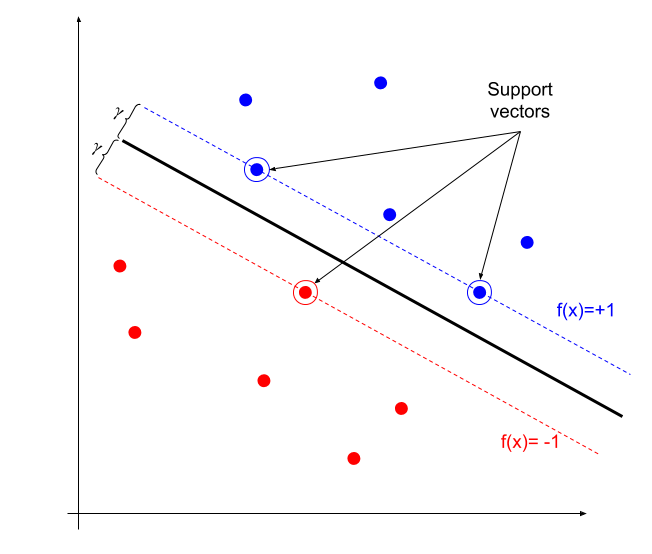
\includegraphics[width=10cm]{support_vectors.png}
\end{center}

Another important consequence of the KKT complementary conditions is that, since $\alpha_i = 0$ of $i \not \in \text{SV}$, then
$$ \gamma = \frac{1}{\norm{\bm w^*}} = \frac{1}{\displaystyle \sqrt{\sum_{i = 1}^N \alpha_i^*}} = \frac{1}{\displaystyle \sqrt{\sum_{i \in \text{SV}} \alpha_i^*}} $$

\section{Kernelized MMC}
Both the dual objective and the decision function have the property that the data only appears inside as an inner product.
This makes it possible to apply MMC to the transformed feature space.

The kernelized version of the dual problem is the following
\begin{align*}
    &\text{Maximize   } \quad \psi(\bm a) = \sum_{i = 1}^N \alpha_i - \frac{1}{2} \sum_{i = 1}^N \sum_{j = 1}^N \alpha_i \alpha_j y_i y_j K(\bm x_i, \bm x_j) \\
    &\text{Subject to } \quad \begin{dcases}
    \sum_{i = 1}^N y_i \alpha_i = 0 \\
    a_i \geq 0
\end{dcases} \quad \text{for } i = 1, \dots, N
\end{align*}

And the discriminant function will be
$$ f(\bm x) = \sum_{i = 1} y_i \alpha_i^* K(\bm x_i, \bm x) + b^* $$
Note that this discriminant function is very similar to the RBF one.
The only advantage brought by SVM is that $\bm \alpha^*$ is sparse, thus only few kernels are needed.

Now the geometric margin $\gamma$ will be defined within the transformed space.

If $K(\cdot)$ satisfies the Mercer's condition (is positive semi-definite), then the optimization problem is again quadratic with a unique solution.

\section{Sparseness}
Another bound on the generalization error can be derived by using the leave-one-out error estimation method.
Since, when a non-SV sample is omitted during training, the result does not change, then we can found the following bound on the number of errors
$$ \text{err}(f) \leq \frac{\#\text{SV}}{N} $$

This is a weak bound because it hash high variance, and depends highly on the training samples.

It can also be used to stabilize the learning process when using semi-supervised learning, i.e. when unlabelled samples are used to improve on the supervised learning training.


\section{Soft Margin Classification}
The MMC only works in the case of linearly separable classes.
This is because it relies on the Margin Bound.
An alternative SVM can be defined starting from the Soft Margin Bound.

To minimize the margin bound we need to minimize the following quantity
\begin{gather*}
    \frac{R^2 + \frac{\norm{\bm \xi}^2}{\norm{\bm w}^2}}{\gamma^2} \\
    \frac{\norm{\bm w}^2 R^2 + \norm{\bm \xi}^2}{\underbrace{\norm{\bm w}^2 \gamma^2}_1} \\
    \norm{\bm w}^2 R^2 + \norm{\bm \xi}^2 \\
    2 R^2 \biggl( \frac{1}{2} \norm{\bm w}^2 + \underbrace{\frac{1}{2 R^2}}_{C/2} \norm{\bm \xi}^2 \biggr) \\
    \frac{1}{2} \norm{\bm w}^2 + \frac{C}{2} \norm{\bm \xi}^2
\end{gather*}

Moreover, the constraints need to be changed with respect to the MMC formulation.
In fact, if the classes are not separable, we can not require that the functional margin be higher then 1.
Instead, we can include the slack term to ``ignore'' the samples that are over the margin, requiring
$$ y_i (\inp{\bm w}{\bm x_i} + b) \geq 1 - \xi_i $$


\subsection{2-norm Soft Margin Classifier}
The primal optimization for the 2-NSMC is thus given by
\begin{align*}
    &\text{Minimize   } \quad \psi(\bm w, \bm xi) = \frac{1}{2} \norm{\bm w}_2^2 + \frac{C}{2} \norm{\bm \xi}_2^2 \\
    &\text{Subject to } \quad \begin{dcases}
    y_i (\inp{\bm w}{\bm x_i} + b) \geq 1 - \xi_i \\
    \xi_i \geq 0
\end{dcases} \quad \text{for } i = 1, \dots, N
\end{align*}
where $C$ is a constant.

The $C$ constant is a hyper-parameter such that, as its value increases, the SVM over-fits.

Again, by starting from the Lagrangian, and imposing stationarity and KKT conditions, we can get to the dual optimization problem
$$ \bm L(\bm w, b, \bm \xi, \bm \alpha) = \sum_{i = 1}^N \alpha_i - \frac{1}{2} \sum_{i = 1}^N \sum_{j = 1}^N y_i y_j \alpha_i \alpha_j \inp{\bm x_i}{\bm x_j} - \frac{1}{2 C} \norm{\bm \alpha}^2 $$
where $\delta_{i, j}$ is the Kronecker delta.

And the dual optimization problem is then
\begin{align*}
    &\text{Maximize   } \quad \psi(\bm \alpha) = \sum_{i = 1}^N \alpha_i - \frac{1}{2} \sum_{i = 1}^N \sum_{j = 1}^N \alpha_i \alpha_j y_i y_j \left( \inp{\bm x_i}{\bm x_j} + \frac{1}{C} \delta_{i, j} \right) \\
    &\text{Subject to } \quad \begin{dcases}
    \sum_{i = 1}^N y_i \alpha_i = 0 \\
    \alpha_i \geq 0
\end{dcases} \quad \text{for } i = 1, \dots, N
\end{align*}

Note that the main difference from the MMC is the $\delta_{i, j}/C$ term, which is added to the diagonal of the Gram matrix.
It is another example of ridge regression.
In fact, here we try to regularize against the presence of noisy data.

In the case where $C \to +\infty$ then the additional term goes to 0, and we return to the initial MMC, and we incur in the risk of over-fitting.

Again, we can easily kernelize the 2NSMC machine by substituting $K(\bm x_i, \bm x_j)$ in place of the simple inner product $\inp{\bm x_i}{\bm x_j}$.
\begin{align*}
    &\text{Maximize   } \quad \psi(\bm \alpha) = \sum_{i = 1}^N \alpha_i - \frac{1}{2} \sum_{i = 1}^N \sum_{j = 1}^N \alpha_i \alpha_j y_i y_j \left( K(\bm x_i, \bm x_j) + \frac{1}{C} \delta_{i, j} \right) \\
    &\text{Subject to } \quad \begin{dcases}
    \sum_{i = 1}^N y_i \alpha_i = 0 \\
    \alpha_i \geq 0
\end{dcases} \quad \text{for } i = 1, \dots, N
\end{align*}

We will now derive the geometrical margin $\gamma = 1/\norm{\bm w}^2$ in the transformed space.
From the KKT conditions we know that, for all $i = 1, \dots, N$
\begin{gather*}
    \alpha_i g_i(\bm w) = 0 \\
    \alpha_i \left[ 1 - \xi_i - y_i (\inp{\bm w}{\bm x_i} + b) \right] = 0 \\
    \alpha_i - \alpha_i \xi_i - \alpha_i y_i \inp{\bm w}{\bm x_i} + \alpha_i y_i b = 0
\end{gather*}
Summing over all the $N$ samples
\begin{gather}
    \sum_{i = 1}^N \alpha_i - \sum_{i = 1}^N  \alpha_i \xi_i - \sum_{i = 1}^N  \alpha_i y_i \inp{\bm w}{\bm x_i} + b \underbrace{\sum_{i = 1}^N \alpha_i y_i}_0 = 0 \\
    \sum_{i = 1}^N \alpha_i - \sum_{i = 1}^N  \alpha_i \xi_i - \inp{\bm w}{\underbrace{\sum_{i = 1}^N \alpha_i y_i \bm x_i}_{\bm w}} + b \underbrace{\sum_{i = 1}^N \alpha_i y_i}_0 = 0 \\
    \inp{\bm w}{\bm w} = \norm{\bm w}^2 = \sum_{i = 1}^N \alpha_i - \sum_{i = 1}^N \alpha_i \xi_i
    \gamma = \frac{1}{\displaystyle \sqrt{\sum_{i = 1}^N \alpha_i - \sum_{i = 1}^N \alpha_i \xi_i}}
\end{gather}

Due to some of the stationarity conditions on the primal lagrangian $\xi_i = \alpha_i/C$, thus

$$ \gamma = \frac{1}{\displaystyle \sqrt{\sum_{i = 1}^N \alpha_i - \frac{1}{C} \norm{\bm \alpha}^2}} $$


\subsubsection{1-Norm Soft Margin Classifier}
The primal form of the 1-NSMC is the following
\begin{align*}
    &\text{Minimize   } \quad \psi(\bm w, \bm \xi) = \frac{1}{2} \norm{\bm w}^2 + C \sum_{i = 1}^N \xi_i \\
    &\text{Subject to } \quad \begin{dcases}
    y_i (\inp{\bm w}{\bm x} + b) \geq 1 - \xi_i = 0 \\
    \xi_i \geq 0
\end{dcases} \quad \text{for } i = 1, \dots, N
\end{align*}

Note that the only difference from the 2-NSMC is the $l_1$-norm and the $1/2$ factor missing from $C$.

We can compute the Lagrangian as
$$ L(\bm w, b, \bm \xi, \bm \alpha, \bm \mu) = \frac{1}{2} \norm{\bm w}^2 + C \sum_{i = 1}^N \xi_i + \sum_{i = 1} \alpha_i [1 - \xi_i  - y_i (\inp{\bm w}{\bm x} + b)] - \sum_{i = 1}^N \mu_i \xi_i $$
with non-negative Lagrangian multipliers $\alpha_i \mu_i$.

The KKT additional conditions are
$$ \begin{dcases}
    \alpha_i [1 - \xi_i  - y_i (\inp{\bm w}{\bm x} + b)] = 0 \\
    \mu_i (-\xi_i) = 0
\end{dcases} $$

By imposing the stationarity of the Lagrangian we obtain
$$ \begin{dcases}
    \pdv{L(\bm w, b, \bm \xi, \bm \alpha, \bm \mu)}{\bm w} = \bm w - \sum_{i = 1}^N \alpha_i y_i \bm x_i = 0 \\
    \pdv{L(\bm w, b, \bm \xi, \bm \alpha, \bm \mu)}{b} = - \sum_{i = 1}^N \alpha_i y_i = 0 \\
    \pdv{L(\bm w, b, \bm \xi, \bm \alpha, \bm \mu)}{\bm \xi} = C - \alpha_i - \mu_i = 0
\end{dcases} \implies
\begin{dcases}
    \bm w = \sum_{i = 1}^N \alpha_i y_i \bm x_i \\
    \sum_{i = 1}^N \alpha_i y_i = 0 \\
    C - \alpha_i - \mu_i = 0
\end{dcases} $$

We will now proceed in removing the primal variables $\bm w, b$ and $\bm x_i$ from the primal Lagrangian to get the dual
\begin{align*}
    L(\bm w, b, \bm \xi, \bm \alpha, \bm \mu)
    &= \frac{1}{2} \norm{\bm w}^2 + C \sum_{i = 1}^N \xi_i + \sum_{i = 1} \alpha_i [1 - \xi_i  - y_i (\inp{\bm w}{\bm x_i} + b)] - \sum_{i = 1}^N \mu_i \xi_i \\
    &= \frac{1}{2} \sum_{i = 1}^N \sum_{j = 1}^N \alpha_i \alpha_j y_i y_j \inp{\bm x_i}{\bm x_j} + \sum_{i = 1}^N \xi_i \underbrace{(C - \alpha_i - \mu_i)}_0 + \sum_{i = 1} \alpha_i - \sum_{i = 1} \alpha_i y_i \inp{\bm w}{\bm x_i} + b \underbrace{\sum_{i = 1} \alpha_i y_i}_0 \\
    &= \sum_{i = 1} \alpha_i - \frac{1}{2} \sum_{i = 1}^N \sum_{j = 1}^N \alpha_i \alpha_j y_i y_j \inp{\bm x_i}{\bm x_j}
\end{align*}

The constraints are
$$ \begin{dcases}
    \sum_{i = 1}^N \alpha_i y_i = 0\\
    \alpha_i \geq 0
\end{dcases} \quad \text{for } i = 1, \dots, N $$

The results so far are identical to the 2-NSMC.
However, there is an additional constraint.

Due to the 2nd primal KKT constraint, if $\xi_i = 0$, then
$$ \mu_i > 0 \implies C - \alpha_i > 0 \implies a_i < C $$
If instead $\xi_i \neq 0$, then
$$ \mu_i = 0 \implies C = \alpha_i $$

Thus, the last constraint to the Lagrangian is $\alpha_i < C$.
The final version of the constraints is the following
$$ \begin{dcases}
    \sum_{i = 1}^N \alpha_i y_i = 0\\
    0 \leq \alpha_i \leq C
\end{dcases} \quad \text{for } i = 1, \dots, N $$

The main difference from the 2-NSMC is thus that the $\alpha_i$ values are bounded.
For this reason, the 1-NSMC is often referred to as \textbf{boxed constraint classifier}.

The KKT constraints for the 1-NSMC are the following
$$ \begin{dcases}
    \alpha_i^* [y_i (\inp{\bm w^*}{\bm x_i} + b^*) - 1 + \xi_i^*] = 0 \\
    \xi_i^* (\alpha_i^* - C) = 0
\end{dcases} \quad \text{for } i = 1, \dots, N $$

Thus
\begin{enumerate}
    \item if the slack $\xi_i$ is not zero, then $\alpha_i^* = C$. These samples form the Non-Margin SV.
    \item if the slack is zero, and the sample $\bm x_i$ is on the margin, then $f(\bm x_i) = 1$, and both conditions are met. In this way, $\alpha_i^*$ can take any value in the allowed range, i.e.
    $$ 0 \leq \alpha_i^* \leq C $$
    These samples form the Margin SV.
    \item if the slack is zero, and the sample $\bm x_i$ is not on the margin, then the second condition is met, but $\alpha_i^*$ must also be zero to satisfy the first condition.
    These samples will be ignored during classification.
\end{enumerate}

\begin{center}
    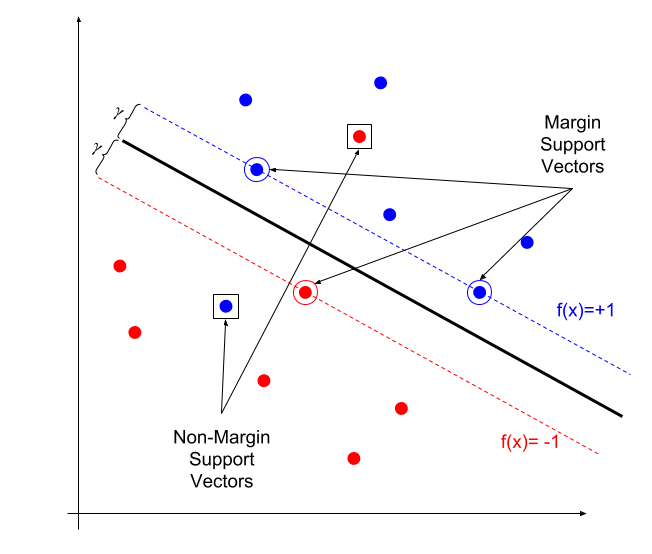
\includegraphics[width=10cm]{support_vectors_1-NSMC.png}
\end{center}

\section{Multiclass SVM}
SVM are formulated for binary classification.
Some multi-class formulation have been presented in the literature.

But the easiest way apply SVM to a multi-class problem is decomposing it into smaller binary classification problems.

The main idea is that of having a lot of binary SVMs in parallel, and then fusing their output with a predefined score function $S(\bm x)$.
Let $C$ be the number of classes
$$ \widehat \omega = \argmax_{i = 1, \dots, C} \{S_i(\bm x)\} $$

\subsection{One-Against-One strategy}
The score function is defined as
$$ S_i(\bm x) = \sum_{\substack{j = 1 \\ j \neq i}}^C \sgn\{f_{i, j}(\bm x)\} $$
where $f_{i, j}(\bm x)$ is the local discriminant function between classes $\omega_i$ and $\omega_j$.

Since $f_{i, j}(\bm x) = -f_{j, i}(\bm x)$, the total number of local discriminant functions (and thus also of parallel SVMs) is
$$ T = \frac{C (C - 1)}{2} $$

\subsubsection{One-Against-All strategy}
The score function is simply the discriminant function $f_i(\bm x)$ which distinguishes between class $\omega_i$ and all the remaining classes.
The number of parallel SVMs required is
$$ T = C $$

This allows for
\begin{itemize}
    \item less SVMs to train, and
    \item no ties.
\end{itemize}

However, it requires solving more complex binary classifications, thus increasing the training time and the prediction time.


\section{Support Vector Regression}
As done for the previous SVMs, the base of SVR is minimizing a generalization bound.
The bound is the linear $\eps$-insensitive loss function, defined as
$$ L_1^\eps(\bm x, y, f) = \max(0, \abs{y - f(\bm x)} - \eps) $$
and its quadratic version is
$$ L_2^\eps(\bm x, y, f) = \max(0, \abs{y - f(\bm x)}^2 - \eps) $$

We can redefine the margin slack vector as
$$ \xi((\bm x_i, y_i), f, \theta, \gamma) = L^{\theta - \gamma}(\bm x_i, y_i, f) $$

We can then try to minimize the sum of the $\eps$-insensitive quadratic losses and the norm of the weight vector $\bm w$.
\begin{align*}
    &\text{Minimize   } \quad \psi(\bm w, \bm \xi, \widehat {\bm \xi}) = \frac{1}{2} \norm{\bm w}^2 + C \sum_{i = 1}^N (\xi_i^2 + \widehat \xi_i^2) \\
    &\text{Subject to } \quad \begin{dcases}
        (\inp{\bm w}{\bm x_i} + b) - y_i \leq \eps + \xi_i \\
        y_i - (\inp{\bm w}{\bm x_i} + b) \leq \eps + \widehat \xi_i \\
        \xi_i \geq 0 \\
        \widehat \xi_i \geq 0
    \end{dcases} \quad \text{for } i = 1, \dots, N
\end{align*}
where $\xi_i$ is the slack when the estimate is higher than the target by more then $\eps$, while $\widehat \xi_i$ is the slack when the estimate is lower than the target by more than $\eps$.

The Support Vectors will now be the samples that lie outside of the $\eps$-insensitive tube.

In the dual linear formulation, we have a box condition on the Lagrange multipliers, like for the SVM.


\section{SVM implementation techniques}
Training a SVM is simply a matter of maximizing a convex quadratic form subject to linear constraints.
This problem is very well studied, and plenty of solutions exist.

However, training might require very large Gram matrices.
To avoid this some methods are used
\begin{itemize}
    \item Gradient Ascent: slow, depends on the learning rate, very simple
    \item Chunking and Decomposition: apply gradient on reduced set, add some more samples and recheck
    \item Sequential Minimal Optimisation: at each iteration, consider only two samples (has an analytical solution)
\end{itemize}

\section{SVM recap}
Pros:
\begin{itemize}
    \item no local minima
    \item few free parameters: Kernel function, regularization parameter $C$ and $\eps$ (in regression only)
    \item fast learning
    \item low sensibility to the curse of dimensionality
    \item very very good performances
\end{itemize}

Cons:
\begin{itemize}
    \item the outcome is not a probabilistic value, but it can be extracted in some way..
\end{itemize}
\end{document}

